\documentclass[11pt,oneside,openany]{book}
\usepackage[T1]{fontenc}
\usepackage[utf8]{inputenc}
\usepackage{lmodern}
\usepackage[a4paper,margin=25mm,headheight=15pt]{geometry}
\usepackage{amsmath,amssymb,amsthm,mathtools,bm}
\usepackage{graphicx,xcolor,booktabs,longtable,tabularx,array,multirow}
\usepackage{enumitem}
\usepackage{microtype}
\usepackage{tikz}
\usetikzlibrary{arrows.meta,positioning,calc}
\usepackage{listings}
\usepackage[most]{tcolorbox}
\usepackage[numbers,sort&compress]{natbib}
\usepackage{fancyhdr}
\usepackage{hyperref}
\usepackage{bookmark}
\definecolor{navy}{HTML}{17334D}
\definecolor{teal}{HTML}{167D8D}
\definecolor{lightteal}{HTML}{EDF7F8}
\definecolor{softgray}{HTML}{F4F6F8}
\definecolor{rust}{HTML}{B05B35}
\hypersetup{colorlinks=true,linkcolor=navy,citecolor=teal,urlcolor=teal,pdftitle={Mathematical Foundations of Neural Dynamics and Geometry},pdfauthor={Prepared with ChatGPT}}
\newcommand{\R}{\mathbb{R}}
\newcommand{\N}{\mathbb{N}}
\newcommand{\Z}{\mathbb{Z}}
\newcommand{\F}{\mathbb{F}}
\newcommand{\E}{\mathbb{E}}
\DeclareMathOperator{\Var}{Var}
\DeclareMathOperator{\Cov}{Cov}
\DeclareMathOperator{\tr}{tr}
\DeclareMathOperator{\rank}{rank}
\DeclareMathOperator{\diag}{diag}
\DeclareMathOperator*{\argmin}{arg\,min}
\DeclareMathOperator*{\argmax}{arg\,max}
\newcommand{\norm}[1]{\left\lVert #1\right\rVert}
\newcommand{\abs}[1]{\left\lvert #1\right\rvert}
\newcommand{\ip}[2]{\left\langle #1,#2\right\rangle}
\newcommand{\dd}{\mathrm{d}}
\newtheorem{theorem}{Theorem}[chapter]
\newtheorem{proposition}[theorem]{Proposition}
\newtheorem{lemma}[theorem]{Lemma}
\theoremstyle{definition}
\newtheorem{definition}[theorem]{Definition}
\newtheorem{example}[theorem]{Example}
\theoremstyle{remark}
\newtheorem{remark}[theorem]{Remark}
\newtheorem{misconception}[theorem]{Common misconception}
\newtcolorbox{insight}[1]{enhanced,breakable,colback=lightteal,colframe=teal,boxrule=.4pt,arc=1mm,title={#1},fonttitle=\bfseries}
\lstset{basicstyle=\ttfamily\footnotesize,keywordstyle=\color{navy}\bfseries,commentstyle=\color{teal},stringstyle=\color{rust},breaklines=true,columns=fullflexible,keepspaces=true,showstringspaces=false,frame=single,rulecolor=\color{black!15},backgroundcolor=\color{softgray},numbers=left,numberstyle=\tiny\color{gray},numbersep=6pt,xleftmargin=1.5em,aboveskip=1em,belowskip=1em}
\setlist{itemsep=3pt,topsep=5pt}
\setlength{\parindent}{1.2em}
\setlength{\parskip}{3pt}
\setlength{\emergencystretch}{3em}
\renewcommand{\arraystretch}{1.18}
\pagestyle{fancy}
\fancyhf{}
\fancyhead[L]{\small\nouppercase{\leftmark}}
\fancyfoot[C]{\thepage}
\renewcommand{\headrulewidth}{.3pt}
\renewcommand{\chaptermark}[1]{\markboth{\thechapter.\ #1}{}}
\setcounter{tocdepth}{1}
\setcounter{secnumdepth}{2}

\begin{document}
\frontmatter
\hypersetup{pageanchor=false}
\begin{titlepage}
\thispagestyle{empty}
\vspace*{1.1cm}
{\sffamily\color{teal}\large MATHEMATICS \quad NEUROSCIENCE \quad MACHINE LEARNING\par}
\vspace{1.1cm}
{\raggedright\sffamily\bfseries\color{navy}\fontsize{29}{35}\selectfont Mathematical Foundations\\of Neural Dynamics\\and Geometry\par}
\vspace{0.9cm}
{\raggedright\sffamily\color{navy}\Large From Dimensionality Reduction\\to Dynamical Systems, Manifolds, and Topology\par}
\vspace{1.1cm}
\noindent{\color{teal}\rule{\textwidth}{1.5pt}}
\vspace{0.6cm}
{\raggedright\large A textbook-style introduction to mathematical objects, computational tools, and the evidence needed to connect them.\par}
\vfill
\begin{tikzpicture}[scale=0.95,>=Stealth]
\draw[navy,thick] (0,0) ellipse (1.6 and 0.65);
\draw[teal,thick,->] (0,1.2) -- (0,0.75);
\draw[teal,thick,->] (0,-1.2) -- (0,-0.75);
\node[navy,align=center] at (0,-1.7) {geometry and attraction};
\draw[navy,thick] (5.2,0) circle (0.8);
\foreach \a in {0,45,...,315}{\fill[teal] ({5.2+0.8*cos(\a)},{0.8*sin(\a)}) circle (0.045);}
\node[navy,align=center] at (5.2,-1.7) {samples and topology};
\draw[navy,thick,->] (8.7,-0.9)--(11.4,-0.9);
\draw[navy,thick,->] (8.7,-0.9)--(8.7,0.9);
\draw[teal,very thick,domain=0:2.35,samples=60] plot ({8.8+\x},{0.65*exp(-1.7*\x)-0.55});
\node[navy,align=center] at (10,-1.7) {dynamics and inference};
\end{tikzpicture}
\vfill
{\sffamily\large Foundations edition\par}
{\sffamily 10 November 2026\par}
\vspace{0.25cm}
{\small Prepared with ChatGPT for an interdisciplinary research audience.\par}
\end{titlepage}
\hypersetup{pageanchor=true}

\chapter*{Preface and scope}
\addcontentsline{toc}{chapter}{Preface and scope}
A scatter plot can look like a ring. A population can be well approximated by two principal components. A recurrent network can return toward a set of states after a perturbation. These are different observations, with different mathematical meanings. The purpose of this book is to make those differences usable: to help a reader derive an analysis, understand its assumptions, and state a conclusion at the strength supported by the data.

We begin with a matrix whose rows are observations and whose columns are measured variables. This familiar object leads to projections and dimensionality reduction. We then introduce state evolution, local stability, charts and tangent spaces, and finally algebraic tools for detecting holes. The application chapters revisit these ideas in neural recordings and artificial networks. The final part makes the inference problem explicit: what distinguishes a mathematical object in a model from evidence for that object in a biological system?

\section*{What this edition contains}
This is a self-contained introductory course and research reference, with thirteen chapters, five mathematical appendices, and nine executable computational tutorials. Central arguments are developed in detail: the PCA optimization problem; local linear stability and its limits; the local meaning of a manifold; chains, boundaries and homology; the distinction between an observation map and a dynamical state; and the design of controls for geometric and dynamical claims. Definitions, modeling assumptions, exact deductions, numerical results, and empirical findings are labeled separately.

The depth is intentionally unequal. Stochastic calculus, general center-manifold and geometric singular-perturbation theory, persistent cohomology coordinate construction, and Koopman spectral theory receive clearly marked introductions. Their general proofs, a full treatment of torsion and integral homology, rigorous finite-sample guarantees for every manifold-learning algorithm, and an exhaustive literature survey are beyond this edition. These extensions are not prerequisites for using the core chapters. References identify where a reader can pursue them. An advanced subsection is a completed introduction to its stated topic, not a claim to replace its specialist textbook.

All computational results in this edition are generated from synthetic data or a small network trained by the included code. They are educational experiments, not reanalyses of the cited biological datasets. The source project includes the scripts, data-generating equations, seeds, numerical summaries, package versions, and figures. The examples make failure modes visible as well as successful recovery. No Python tutorial infers a biological circuit from simulated evidence.

\section*{How definitions, proofs, and examples are used}
A definition fixes a convention; it is not an empirical claim. A theorem states a conclusion conditional on its hypotheses. A worked example shows the calculation in a system simple enough to check. An empirical study can provide support for a model without establishing every hypothesis of a theorem. Each use has value, but substituting one for another obscures the scientific question.

The first occurrence of an unfamiliar concept includes its intuitive purpose and formal meaning. Appendices give short prerequisite refreshers, while the glossary points back to the full development. Readers should not feel obliged to memorize every term before proceeding. A useful learning cycle is to read a definition, work one example, run the associated tutorial, and return to the definition with a concrete object in mind.

Proof sketches are labeled as such. They explain the main logical steps while indicating what has been omitted. Numerical checks validate an implementation against a specified example; they are not proofs of a theorem. When a fixed-point search finds several roots, for instance, its residual check can establish that each candidate is approximately a root, but cannot establish that all roots have been found.

\begin{insight}{The question to keep asking}
What is the proposed mathematical object? What is actually observed? Which analysis connects them? What alternative could produce the same result? What additional measurement or intervention would distinguish it?
\end{insight}

\chapter*{Curriculum, notation, and reading routes}
\addcontentsline{toc}{chapter}{Curriculum, notation, and reading routes}
\section*{A dependency-aware curriculum}
The chapters follow a logical dependency order rather than a ranking of fashionable techniques. It is possible to use PCA without understanding homology; it is not possible to interpret a persistent homology class carefully without knowing what a cycle, a boundary, and a filtration are. Chapters 3 and 4 therefore supply the topology needed by the later applications, while Chapter 5 explains why geometric recovery and dynamical recovery are separate problems.

\small
\begin{longtable}{>{\raggedright\arraybackslash}p{0.06\textwidth}>{\raggedright\arraybackslash}p{0.25\textwidth}>{\raggedright\arraybackslash}p{0.17\textwidth}>{\raggedright\arraybackslash}p{0.41\textwidth}}
\toprule
Ch. & Topic & Main prerequisites & Capability developed \\
\midrule\endhead
1 & Data and dimensionality & Elementary algebra; App.~A & Derive PCA and compare linear, intrinsic, and effective dimensions. \\
2 & Dynamical systems & Calculus; App.~B & Define a state, locate equilibria, and assess local stability. \\
3 & Manifolds and geometry & Ch.~1; basic sets & Separate local coordinates, embedding, metric, and topology. \\
4 & Topology and persistence & Ch.~3 topology; App.~D & Compute simple homology and interpret persistence with explicit coefficients and scale. \\
5 & Dynamics on geometric sets & Chs.~2--4 & Distinguish invariant, stable, center, and slow manifolds and observation geometry. \\
6 & Population analysis & Chs.~1--2; App.~C & Understand latent statistical models, preprocessing, and validation. \\
7 & Neural attractor models & Chs.~2, 5 & Relate recurrent mechanisms to contraction, memory, and perturbations. \\
8 & Neural representation geometry & Chs.~1, 3, 5 & Evaluate manifold and alignment claims under an observation model. \\
9 & Neural topological analysis & Chs.~4, 6, 8 & Specify an end-to-end pipeline, statistic, and relevant null. \\
10 & Artificial neural networks & Chs.~2, 5--8 & Analyze complete hidden states and separate inference from learning. \\
11 & Computational tutorials & Topic-specific chapters & Reproduce known-ground-truth examples and test competing explanations. \\
12 & Evaluating mathematical claims & Chs.~1--10 & Match the strength of a conclusion to its evidence. \\
13 & Literature case studies & Ch.~12 framework & Read influential papers without weakening or inflating their claims. \\
\bottomrule
\end{longtable}
\normalsize

\section*{Three reading routes}
\textbf{The foundations route} follows Chapters 1--5, consulting the appendices as needed, and then uses the relevant application chapters. This is the most systematic route for a reader new to differential equations and topology.

\textbf{The experimental data route} begins with Chapters 1 and 6, then reads Chapters 3--4 before Chapters 8--9. Chapter 12 should accompany every analysis decision. Chapter 2 and the perturbation examples in Chapter 7 prevent a descriptive population embedding from being mistaken for an attractor model.

\textbf{The recurrent-network route} reads Chapters 1--2, 5, 7, and 10, with Tutorials 3--5, 8, and 9. Chapters 3--4 become essential when the question concerns the topology of a family of hidden states, rather than the stability of a particular computation. This route is also useful when studying changes in representations across training checkpoints.

\section*{Notation used throughout}
\begin{longtable}{>{\raggedright\arraybackslash}p{0.19\textwidth}>{\raggedright\arraybackslash}p{0.71\textwidth}}
\toprule Symbol & Meaning \\
\midrule\endhead
$X\in\R^{n\times p}$ & Data matrix: $n$ observations in rows, $p$ features or neurons in columns. \\
$X_c$, $C$ & Centered data and sample covariance $C=X_c^TX_c/(n-1)$. \\
$d$, $k$, $p$ & Intrinsic dimension, retained linear dimension, and ambient dimension. Local contexts specify other uses explicitly. \\
$\gamma_j$ & Covariance eigenvalues, sorted in decreasing order when discussing dimension. \\
$x(t)$, $h_t$ & Continuous state and discrete hidden state. A full state must contain all variables needed for its evolution given inputs. \\
$y$, $g$ & Observed activity and observation map, often $y=g(x)+\eta$. \\
$u(t)$, $u_t$ & Externally specified input. A fixed input is written $u_0$. \\
$f$, $F$ & Continuous vector field $\dot x=f(x,u)$ and discrete update $x_{t+1}=F(x_t,u_t)$. \\
$J$, $\lambda$ & Jacobian of a vector field or update map, and its eigenvalues. \\
$\theta$ & Parameters of a learned model; in an explicitly circular example, an angle. The local definition disambiguates the use. \\
$\tau$ & Time constant; its units match the time variable in an ODE. \\
$M$, $T_xM$ & Manifold and tangent space at $x$. \\
$H_q(K;\F)$, $\beta_q$ & Homology of complex $K$ in degree $q$ over field $\F$, and its dimension. \\
$\epsilon$, $r$ & Rips maximum edge length and \v{C}ech ball radius, respectively. A factor of two matters when comparing conventions. \\
$\F_2$, $\F_\ell$ & Finite fields of two elements or prime order $\ell$. Persistent homology tutorials use $\F_2$. \\
$\rho(J)$ & Spectral radius: maximum absolute eigenvalue of a square matrix. \\
$\norm{\cdot}$, $\ip{\cdot}{\cdot}$ & Euclidean norm and inner product unless another metric is specified. \\
\bottomrule
\end{longtable}

\section*{A note on axes, units, and coordinates}
A coordinate is not a mechanism. PCA axes may change sign without changing the fitted subspace. Latent coordinates may rotate while a model's predictions stay the same. A change from milliseconds to seconds rescales the numerical entries of a continuous-time Jacobian, but it does not change the sign of their real parts. A discrete-time multiplier, in contrast, is dimensionless and must be compared with the unit circle. Throughout the book, such invariances are used as sanity checks.

An equation is interpreted in its declared coordinate system and observation model. Standardizing each neuron changes Euclidean distances; nonlinear embedding changes geometry; averaging trials changes the distribution being analyzed. There is no universally neutral preprocessing. The useful question is which scientific variation the chosen operation retains and which it removes.

\tableofcontents
\listoffigures
\mainmatter
\part{Mathematical foundations}
\chapter{Data, vector spaces, and dimensionality reduction}\label{ch:01}
\begin{insight}{Learning objectives}
Represent observations without confusing samples with coordinates; derive PCA from projection error; distinguish four meanings of dimension; compare the mathematical quantities preserved by common embedding methods; and recognize what a low-dimensional picture cannot establish.
\end{insight}

\section{What is a dimension of data?}
Suppose two instruments measure the same fluctuating signal, one at twice the gain of the other. Their output is a point $(s,2s)$ in a two-dimensional plotting space, but one number $s$ determines both readings. A third instrument measuring $s^2$ produces $(s,2s,s^2)$. There is still one freely varying parameter, yet the points generally do not lie on a line. The first example is linearly one-dimensional; the second is intrinsically one-dimensional but curved. Distinguishing these statements is the starting point of this book.

Write $n$ observations of $p$ variables as
\begin{equation}\label{eq:data-matrix}
X=\begin{bmatrix}x_1^T\\\vdots\\x_n^T\end{bmatrix}\in\R^{n\times p},\qquad
x_i=(x_{i1},\ldots,x_{ip})^T\in\R^p.
\end{equation}
The superscript $T$ means transpose. Rows are observations; columns are variables. A neural example has one row per time bin and one column per recorded neuron. The ambient dimension is $p$, independently of the number of observations. Having $n<p$ restricts the rank of the observed matrix, but does not establish that the underlying biological system has dimension at most $n$.

\subsection{Spaces, bases, and rank}
A real vector space is a set in which vectors can be added and multiplied by real numbers, subject to the familiar associative, distributive, identity, and inverse rules. A \emph{subspace} of $\R^p$ contains zero and is closed under these operations. The span of vectors $v_1,\ldots,v_k$ is the set of their linear combinations, $\sum_j a_jv_j$. These vectors are linearly independent when the only combination giving zero has every $a_j=0$. A basis is an independent spanning set; its number of elements is the dimension. Different bases provide different coordinates for the same subspace.

A shifted plane $\mu+S$ is an affine subspace. It need not contain zero. This distinction explains why centering is part of ordinary PCA. For a matrix $A\in\R^{m\times p}$, its image is $\{Av:v\in\R^p\}$ and its null space is $\{v:Av=0\}$. Its rank is the dimension of its image. The rank--nullity identity is
\begin{equation}
\rank(A)+\dim\ker(A)=p.
\end{equation}
To see why, choose a basis of the null space and extend it to a basis of the domain. The images of the added basis vectors form a basis of the image. This elementary identity becomes useful when asking how many hidden changes a measurement map cannot detect.

\subsection{Length, angles, and projection}
An inner product assigns a symmetric bilinear quantity $\ip{v}{w}$ with $\ip{v}{v}>0$ for nonzero $v$. The Euclidean choice is $v^Tw$. Its norm is $\norm{v}_2=\sqrt{v^Tv}$; orthogonality means $v^Tw=0$. If the columns of $V\in\R^{p\times k}$ are orthonormal, $V^TV=I_k$, then
\begin{equation}\label{eq:orth-projection}
P=VV^T,\qquad z=V^Tx,\qquad \widehat x=Vz=Px
\end{equation}
are the orthogonal projection matrix, coordinates, and reconstruction. Indeed $P^T=P$, $P^2=P$, and $V^T(x-Px)=0$: the residual is perpendicular to the retained subspace. Consequently
$\norm{x}_2^2=\norm{Px}_2^2+\norm{x-Px}_2^2$.
This Pythagorean identity connects retained variance with reconstruction error.

A norm satisfies positivity, absolute homogeneity, and the triangle inequality. Not every norm comes from an inner product. For example $\norm{x}_1=\sum_j|x_j|$ is a legitimate norm but does not support the same orthogonal-projection geometry. An algorithm's use of distance therefore makes a substantive choice, rather than merely choosing units for the final plot.

\section{Covariance and singular values}
Let $\bar x=n^{-1}\sum_i x_i$, and let $X_c$ contain rows $(x_i-\bar x)^T$. For $n\geq2$, the sample covariance is
\begin{equation}\label{eq:sample-covariance}
C=\frac{1}{n-1}X_c^TX_c,\qquad C_{ab}=\frac{1}{n-1}\sum_i(x_{ia}-\bar x_a)(x_{ib}-\bar x_b).
\end{equation}
For independent identically distributed observations with finite second moments this is an unbiased covariance estimator. For temporally correlated observations the same matrix describes sample dispersion, but familiar independent-sample uncertainty formulas no longer apply.

$C$ is symmetric and positive semidefinite, since $v^TCv=\norm{X_cv}_2^2/(n-1)\geq0$. The spectral theorem gives an orthonormal eigenbasis:
\begin{equation}
C=V\diag(\gamma_1,\ldots,\gamma_p)V^T,\qquad
\gamma_1\geq\cdots\geq\gamma_p\geq0.
\end{equation}
Here an eigenvector $v_j$ is a direction preserved by multiplication by $C$, and $\gamma_j$ is its eigenvalue. In general, a nonsymmetric matrix need not have a real orthogonal eigenbasis. The spectral theorem is being used because covariance has the required symmetry.

The singular value decomposition, which does not require symmetry, writes any real matrix as $X_c=U\Sigma V^T$, with orthonormal singular vectors and nonnegative singular values $s_j$ on the rectangular diagonal of $\Sigma$. Multiplying out gives $C=V\Sigma^T\Sigma V^T/(n-1)$ and therefore
\begin{equation}\label{eq:svd-pca}
\gamma_j=s_j^2/(n-1).
\end{equation}
Computing PCA through the SVD of $X_c$ often avoids forming a large covariance matrix and avoids squaring its numerical condition number.

If $D=\diag(C_{11},\ldots,C_{pp})$ has positive diagonal entries, the correlation matrix is $D^{-1/2}CD^{-1/2}$. PCA on this matrix is PCA after standardizing each variable to unit sample variance. A variable with zero sample variance requires separate treatment. Standardization changes the question: a small-variance variable receives as much marginal weight as a large-variance variable. Neither covariance-PCA nor correlation-PCA is universally correct.

\section{Deriving principal component analysis}
\subsection{One component: maximize variance}
The scalar coordinate in unit direction $v$ is $z_i=v^T(x_i-\bar x)$. Its sample variance is $v^TCv$. The constrained optimization is
\begin{equation}
\max_{v^Tv=1}v^TCv.
\end{equation}
The Lagrangian $L(v,\lambda)=v^TCv-\lambda(v^Tv-1)$ has stationary condition $2Cv-2\lambda v=0$. Thus stationary directions are eigenvectors. Expanding any unit vector in the eigenbasis, $v=\sum_j a_jv_j$ with $\sum_j a_j^2=1$, gives
$v^TCv=\sum_j\gamma_ja_j^2\leq\gamma_1$.
The maximizing direction is a leading eigenvector. If the leading eigenvalue is repeated, the direction is not unique.

\subsection{Several components: minimize reconstruction error}
For $V_k^TV_k=I_k$, minimize the squared Frobenius norm, the sum of squared matrix entries:
\begin{align}
\norm{X_c-X_cV_kV_k^T}_F^2
&=\norm{X_c}_F^2-\norm{X_cV_k}_F^2\\
&=(n-1)\{\tr(C)-\tr(V_k^TCV_k)\}.\label{eq:pca-objective}
\end{align}
The first equality applies the projection identity to every row. Therefore minimizing error is equivalent to maximizing the sum of variances of $k$ orthogonal coordinates.

\begin{theorem}[Optimal linear reconstruction]\label{thm:pca}
For centered $X_c$ and $0\leq k\leq\min(n,p)$, projection onto $k$ leading right singular vectors minimizes \eqref{eq:pca-objective}. Its error is $\sum_{j>k}s_j^2$. The truncated SVD $U_k\Sigma_kV_k^T$ also minimizes $\norm{X_c-B}_F$ among all matrices $B$ of rank at most $k$.
\end{theorem}
\begin{proof}[Proof of the projection statement; sketch of the rank statement]
In a covariance eigenbasis, $\tr(V_k^TCV_k)=\sum_j\gamma_jw_j$, where $w_j=\norm{V_k^Tv_j}_2^2$, $0\leq w_j\leq1$, and $\sum_jw_j=k$. This weighted sum cannot exceed $\sum_{j=1}^k\gamma_j$. Choosing the leading eigenvectors attains it. For arbitrary rank-$k$ $B$, let $S$ be its row space. Each row of $X_c$ is approximated at least as well by its orthogonal projection onto $S$ as by the corresponding row of $B$. The first result then bounds the error of every such $B$.
\end{proof}

The explained variance ratio of component $j$ is $\gamma_j/\sum_l\gamma_l$, provided total variance is nonzero. A chosen threshold, for example 90\%, defines a \emph{variance-threshold dimension}, not an intrinsic dimension theorem.

\begin{example}[A complete two-variable calculation]
For $C=\left[\begin{smallmatrix}2&1\\1&2\end{smallmatrix}\right]$, the eigenvectors are $v_1=(1,1)^T/\sqrt2$ and $v_2=(1,-1)^T/\sqrt2$, with eigenvalues 3 and 1. The first PC captures $3/4$ of the variance. A centered observation $(2,0)$ has first-PC score $\sqrt2$ and reconstruction $(1,1)$. Its discarded residual $(1,-1)$ has squared length 2. Choosing a different basis within the same retained subspace changes coordinates, not reconstructions.
\end{example}

\begin{misconception}
A principal component is neither a particular neuron nor automatically a causal variable. Its sign is arbitrary, and tied eigenvalues allow rotations within their eigenspace. A task-relevant signal can have small variance and be discarded by an optimal variance-preserving projection.
\end{misconception}

\section{Four different dimensions}
\begin{definition}[Dimension terminology]
The \emph{ambient dimension} is the number of coordinates in the measurement space. The \emph{linear dimension} of exact centered data is $\rank(X_c)$; approximate linear dimension requires an explicit error or variance criterion. The \emph{intrinsic dimension} of a smooth manifold is its local number of independent coordinates (Chapter~\ref{ch:03}). An \emph{effective dimension} summarizes a spectrum or task-dependent notion of complexity and need not be an integer.
\end{definition}
For nonnegative covariance eigenvalues with positive sum, the participation ratio is
\begin{equation}\label{eq:participation-ratio}
d_{\rm PR}=\frac{(\sum_j\gamma_j)^2}{\sum_j\gamma_j^2}
=\frac{1}{\sum_jq_j^2},\qquad q_j=\frac{\gamma_j}{\sum_l\gamma_l}.
\end{equation}
If $r$ eigenvalues are nonzero, $1\leq d_{\rm PR}\leq r$. The upper bound follows from Cauchy--Schwarz, $(\sum_j\gamma_j)^2\leq r\sum_j\gamma_j^2$. Equality at the upper bound requires equal nonzero eigenvalues. The spectral entropy dimension $\exp(-\sum_jq_j\log q_j)$ is another summary; it is not generally equal to the participation ratio.

\begin{example}[A circle defeats a single linear dimension]
Let $x(\theta)=(\cos\theta,\sin\theta)$ with $\theta$ uniform on $[0,2\pi)$. The covariance is $I_2/2$, so $d_{\rm PR}=2$, and two PCs are required for exact reconstruction. Yet a short arc needs only the angle as a local coordinate: intrinsic dimension is one. No continuous injective real-valued global coordinate can represent the entire circle without a cut. Topology, rather than an inadequate optimization algorithm, creates this obstruction.
\end{example}

Noise makes these differences sharper. If $y=s+\eta$ with independent zero-mean isotropic noise of covariance $\sigma^2I_p$, then $C_y=C_s+\sigma^2I_p$. Every covariance eigenvalue is increased by $\sigma^2$. A smooth curve with full-support additive Gaussian noise has a full-dimensional observation distribution; calling it a ``one-dimensional noisy manifold'' is a model for its signal component, not a literal statement about the support of $y$.

\subsection{Estimating local dimension}
One approach fits PCA in neighborhoods. For a smooth $d$-dimensional surface and sufficiently small neighborhoods, tangent variation dominates curvature, but neighborhoods that are too small are dominated by noise and sampling variability. Thus the useful scale lies between noise and curvature scales, if such a range exists.

Distance estimators use the fact that volume of a small $d$-dimensional ball scales as $r^d$. Write $T_j(x)$ for the distance from $x$ to its $j$th nearest neighbor. A common local likelihood estimator is
\begin{equation}\label{eq:local-dimension}
\widehat d_k(x)=\left[\frac{1}{k-1}\sum_{j=1}^{k-1}\log\frac{T_k(x)}{T_j(x)}\right]^{-1}.
\end{equation}
The approximation treats local density as constant and neighbor counts as a Poisson process; finite-sample bias corrections and pooling choices matter \citep{levina2004}. Duplicates, boundaries, strongly varying density, correlated sampling, and measurement noise violate parts of this approximation. Plotting estimates across a range of $k$, sample sizes, and noise levels is more informative than one reported integer. A plateau across scales is supporting evidence, not a proof of smooth manifold structure.

\section{Distances encode a scientific choice}
Euclidean distance measures squared coordinate differences. For a positive definite matrix $M$, $d_M(x,y)=\sqrt{(x-y)^TM(x-y)}$ is a metric: it is Euclidean distance after an invertible linear change of coordinates. A covariance-based Mahalanobis metric chooses $M=C^{-1}$, but estimating and inverting $C$ can be unstable; regularization changes the metric. If $M$ is only positive semidefinite, distinct points may have distance zero, giving a pseudometric rather than a metric.

Cosine similarity compares direction after dividing by vector lengths. The quantity $1-\cos\theta$ is widely called a distance but does not generally satisfy the triangle inequality. Angular distance on normalized nonzero vectors is a metric. Correlation distance additionally subtracts each vector's mean. These choices remove different information: overall firing-rate magnitude may be signal in one experiment and nuisance in another. Distance-dependent topology and clustering inherit these choices.

\section{Beyond PCA: what is each algorithm trying to preserve?}
An embedding is a collection of coordinates $z_i\in\R^k$ in this computational section. It is not automatically an embedding in the differential-geometric sense of Chapter~\ref{ch:03}. We state the main objectives so that attractive figures can be judged against what was actually optimized.

\subsection{Multidimensional scaling and Isomap}
For Euclidean pairwise distances $D_{ij}=\norm{x_i-x_j}$, define $H=I_n-\mathbf1\mathbf1^T/n$. Double-centering squared distances gives
\begin{equation}\label{eq:classical-mds}
B=-\tfrac12 H(D^{\circ2})H=X_cX_c^T.
\end{equation}
Here $D^{\circ2}$ means entrywise squares. Expanding $D_{ij}^2=\norm{x_i}^2+\norm{x_j}^2-2x_i^Tx_j$ proves the identity: centering annihilates the separate row and column norm terms. Classical MDS uses the leading positive eigenpairs of $B$ as coordinates. For Euclidean distances, these are PCA scores up to an orthogonal transformation. With arbitrary dissimilarities, negative eigenvalues show that exact Euclidean realization is impossible. Classical MDS minimizes a Gram-matrix approximation error; \emph{metric stress MDS}, which minimizes weighted errors in distances, is a different objective.

Isomap forms a neighborhood graph, weights edges by observed distances, computes graph shortest-path distances, and applies classical MDS \citep{tenenbaum2000}. If sampling is dense, neighborhoods are sufficiently local, and the manifold geometry admits the desired flat parameterization, these graph distances can approximate intrinsic distances. Short-circuit edges between nearby folds corrupt them; too few edges disconnect the graph. A curved sphere does not become globally isometric to a Euclidean plane simply because its graph distances are estimated accurately.

\subsection{Locally linear embedding}
LLE first finds local reconstruction weights with $w_{ij}=0$ outside each neighborhood and $\sum_jw_{ij}=1$, minimizing $\sum_i\norm{x_i-\sum_jw_{ij}x_j}^2$. It then holds the weights fixed and minimizes
\begin{equation}
\sum_i\norm{z_i-\sum_jw_{ij}z_j}^2,
\quad \sum_i z_i=0,\quad n^{-1}Z^TZ=I_k.
\end{equation}
Centering and scaling constraints prevent the collapsed solution $z_i=0$. The second step is a sparse eigenproblem \citep{roweis2000}. Preserving local affine reconstruction coefficients can reveal smooth structure, but depends on neighborhoods, numerical regularization, and sampling. It does not directly preserve all geodesic distances.

\subsection{Diffusion maps}
A nonnegative symmetric kernel, for example $K_{ij}=\exp[-\norm{x_i-x_j}^2/\epsilon]$, defines weighted connectivity. Normalize rows to get a Markov matrix $P_{ij}=K_{ij}/\sum_lK_{il}$, whose rows sum to one. Its powers describe a random walk on observations, not necessarily physical neural time. For a connected reversible chain with strictly positive stationary probabilities $\pi_j$, the diffusion distance at walk time $m$ is
\begin{equation}
D_m(i,l)^2=\sum_j\frac{(P^m_{ij}-P^m_{lj})^2}{\pi_j}
=\sum_{a\geq1}\lambda_a^{2m}(\psi_a(i)-\psi_a(l))^2,
\end{equation}
using right eigenvectors normalized in the $\pi$-weighted inner product and excluding the constant eigenvector. Truncating coordinates $\lambda_a^m\psi_a(i)$ approximates this distance. Kernel normalization controls how sampling density affects the limiting operator \citep{coifman2006}. Without assumptions connecting the sampling process to real dynamics, diffusion coordinates are geometric summaries, not recovered dynamical modes.

\subsection{t-SNE and UMAP}
t-SNE converts local distances into affinities. For $j\ne i$, $p_{j|i}$ is proportional to $\exp[-\norm{x_i-x_j}^2/(2\sigma_i^2)]$, normalized over $j$. Local bandwidths are chosen using perplexity, an effective neighbor-count parameter. Set $p_{ij}=(p_{j|i}+p_{i|j})/(2n)$ and $q_{ij}\propto(1+\norm{z_i-z_j}^2)^{-1}$. The optimized loss is
\begin{equation}
\operatorname{KL}(P\|Q)=\sum_{i\ne j}p_{ij}\log(p_{ij}/q_{ij}).
\end{equation}
Large original affinities receive strong protection; global distances and displayed cluster sizes have no corresponding general preservation guarantee \citep{vandermaaten2008}.

UMAP combines adaptive neighborhood affinities into symmetric fuzzy edge weights $w_{ij}$ and fits low-dimensional affinities $v_{ij}=(1+a\norm{z_i-z_j}^{2b})^{-1}$. Its nominal fuzzy-set cross-entropy, up to constants independent of $Z$, is
\begin{equation}
-\sum_{i<j}\{w_{ij}\log v_{ij}+(1-w_{ij})\log(1-v_{ij})\}.
\end{equation}
Practical optimization uses sampled edges and negative samples, so the implementation's effective weighting need not equal full all-pairs optimization. Neighborhood size, minimum-distance settings, and random initialization change the output. The method's mathematical motivation does not certify that input data form a manifold or that a displayed hole reflects the original data \citep{mcinnes2018}.

\begin{table}[htbp]
\centering\small
\begin{tabularx}{\linewidth}{p{.16\linewidth}XX}
\toprule Method & Main preserved or optimized quantity & Principal interpretive limitation\\\midrule
PCA & Orthogonal linear reconstruction; retained variance & Curved signals may require many PCs; low variance need not be unimportant.\\
Classical MDS & Centered Gram matrix inferred from distances & Negative eigenvalues or truncation indicate geometric distortion.\\
Isomap & Graph estimates of geodesic distance, then MDS & Needs reliable neighborhoods and compatible target geometry.\\
LLE & Local affine reconstruction weights & Neighborhoods and regularization determine local constraints.\\
Diffusion maps & Random-walk connectivity at a chosen scale & Walk time is an analysis parameter; density normalization matters.\\
t-SNE & KL divergence between affinities & Distances between separated clusters are not generally calibrated.\\
UMAP & Fuzzy neighborhood affinities with sampled optimization & A two-dimensional layout is not a topology certificate.\\\bottomrule
\end{tabularx}
\caption{Different dimensionality reductions answer different mathematical questions.}
\end{table}

\section{Worked analysis: a curve, noise, and an honest conclusion}
Consider $s\sim\operatorname{Uniform}[-1,1]$ and $x=(s,s^2)$. Centering gives mean $(0,1/3)$ and covariance $\diag(1/3,4/45)$, because $\E[s^2]=1/3$, $\E[s^4]=1/5$, and odd moments vanish. The first PC explains $(1/3)/(1/3+4/45)=15/19$ of variance. Linear rank is two, while the map $s\mapsto(s,s^2)$ is a smooth injective curve with nonzero derivative. Add isotropic observation noise and both eigenvalues rise. One should report the retained-variance curve, local dimension estimates over scales, noise assumptions, and held-out reconstruction. Calling the cloud ``two-dimensional'' or ``one-dimensional'' without specifying which meaning hides the central distinction.

A useful held-out procedure fits centering, scaling, and axes on training observations, then reconstructs independent test observations. For time series, split by trials or contiguous blocks to avoid leakage from near-identical adjacent samples. Choose the dimension using training/validation data, reserve a final test set, and compare with explicit noise and sampling controls. This estimates predictive usefulness of a representation; it does not by itself prove a manifold theorem.

\section{Exercises}
\begin{enumerate}
\item \textbf{Introductory.} Compute the PCA axes, explained variance, and participation ratio of $\diag(9,1,0)$. Explain why three numbers are needed to describe ambient, exact linear, and effective dimension.
\item \textbf{Introductory.} Show that scaling one variable changes covariance-PCA. Give a two-variable example in which the leading PC changes after standardization.
\item \textbf{Intermediate.} Derive \eqref{eq:classical-mds} explicitly and show why translating all observations leaves the distances unchanged.
\item \textbf{Intermediate.} For $p$-dimensional isotropic noise added to a rank-one signal with covariance eigenvalue $a$, derive $d_{\rm PR}$ as a function of $a$ and $\sigma^2$. Check both noise limits.
\item \textbf{Intermediate.} Sample a circle nonuniformly. Compare global PCA and neighborhood-based dimension estimates. Separate geometric effects from sampling-density effects.
\item \textbf{Advanced.} Explain why no continuous one-to-one map $S^1\to\R$ exists, using compactness and the effect of removing a point. Identify the assumption that an attempted one-dimensional embedding must violate.
\item \textbf{Advanced.} Design a blocked cross-validation scheme for choosing both smoothing bandwidth and latent dimension. State which transformations must be refitted inside each training split.
\end{enumerate}

\section{Summary and further reading}
PCA is an exact solution to a specified linear reconstruction problem. Its variance spectrum is not an intrinsic-dimension estimator without further assumptions. Nonlinear methods optimize different neighborhood, distance, or affinity objectives; none turns visualization into proof. The primary method papers provide the relevant objectives and assumptions: Isomap \citep{tenenbaum2000}, LLE \citep{roweis2000}, diffusion maps \citep{coifman2006}, t-SNE \citep{vandermaaten2008}, UMAP \citep{mcinnes2018}, and neighbor-based dimension estimation \citep{levina2004}. Chapter~\ref{ch:03} supplies the geometric meaning of the word manifold; Chapter~\ref{ch:06} adds observation models and neural preprocessing.

\chapter{Foundations of dynamical systems}\label{ch:02}
\begin{insight}{Learning objectives}
Distinguish state, measurement, and input; solve and linearize basic evolution laws; apply stability criteria with their correct hypotheses; define attraction of sets; distinguish oscillation from a limit cycle; and understand why noise changes the meaning of persistence and stability.
\end{insight}

\section{From a picture of observations to a law of motion}
A scatter plot says where observations occur. It does not say where the system goes next. The same circular cloud could be traversed clockwise, counterclockwise, irregularly under external input, or by independent sampling. A dynamical model adds an evolution rule.

A \emph{state} contains enough information, under the proposed model and specified future inputs, to determine subsequent evolution or its probability law. Position alone is not a state for a freely moving mass: velocity is also needed. Similarly, a projection of neural activity is not automatically a complete neural state. Calling a variable a state is a modeling claim about sufficiency.

A discrete-time autonomous system is $x_{t+1}=F(x_t)$, with $x_t$ in a state space $S$ and $F:S\to S$. ``Autonomous'' means that the rule has no explicit time dependence. With input, write $x_{t+1}=F(x_t,u_t)$; fixing $u_t=u_0$ defines a different autonomous system for each $u_0$. A continuous-time ordinary differential equation (ODE) is
\begin{equation}\label{eq:ode}
\dot x(t)=f(x(t)),\qquad x(0)=x_0,
\end{equation}
where the dot denotes derivative with respect to time. The vector field $f$ specifies instantaneous velocity. If $x$ is measured in firing-rate units and time in seconds, $f$ has firing-rate units per second.

A non-autonomous ODE has explicit time dependence, $\dot x=f(x,t)$, or a specified time-varying input $\dot x=f(x,u(t))$. For example $\dot x=-x+\sin t$ is continually driven even after initial transients disappear. Its evolution depends on both starting time and elapsed time, so the solution maps generally have two time indices rather than a one-parameter flow. One can formally make it autonomous by adding a clock state $\dot s=1$, but the enlarged state space and its invariant sets must then be interpreted accordingly. Holding an input fixed for fixed-point analysis is a well-defined experimental condition, not a claim that the original task had constant input.


\subsection{Why existence and uniqueness matter}
\begin{theorem}[Local well-posedness, standard version]
If $f$ is continuous and locally Lipschitz in $x$ on an open set $U\subset\R^p$, then through every $x_0\in U$ there is a unique local solution of \eqref{eq:ode}. A continuously differentiable vector field is locally Lipschitz. Solutions extend while they remain in compact subsets of the domain; global existence needs additional control preventing escape or blow-up.
\end{theorem}
\begin{proof}[Proof idea]
Integrate the ODE to obtain $x(t)=x_0+\int_0^t f(x(s))\,ds$. On a sufficiently short interval the right-hand side is a contraction on continuous paths in a small ball: two paths become closer by at most a Lipschitz constant times the interval length. Iterating it converges to a unique fixed path. The same argument can be restarted along that path. Detailed hypotheses and continuation arguments are developed by \citet{teschl2012}.
\end{proof}

Continuity alone is insufficient. The equation $\dot x=2\sqrt{|x|}$ with $x(0)=0$ admits a solution that stays at zero until any chosen time $a\geq0$ and then follows $(t-a)^2$. In contrast, $\dot x=x^2$ is smooth but the solution $x(t)=x_0/(1-x_0t)$ blows up in finite positive time for $x_0>0$. Local well-posedness does not guarantee a global flow.

Where solutions exist, define $\phi_t(x_0)=x(t)$. Uniqueness gives $\phi_0=\operatorname{id}$ and $\phi_{t+s}=\phi_t\circ\phi_s$ whenever both sides are defined. A global flow permits positive and negative times; a semiflow requires only nonnegative times. A \emph{trajectory} is the time-parameterized solution, while its \emph{orbit} is the set of points it visits. A phase portrait shows representative trajectories and the vector field. It should not be mistaken for an ensemble of independently sampled observations.

\section{Equilibria and linear systems}
An equilibrium $x_*$ satisfies $f(x_*)=0$, hence $x(t)=x_*$ is a constant solution. A discrete fixed point satisfies $F(x_*)=x_*$. The equations differ because an ODE specifies velocity and a map specifies the next state.

\begin{example}[A one-dimensional decay]
For $\tau\dot x=-x+b$, where $\tau>0$ is a time constant, $x_*=b$ and $x(t)=b+(x_0-b)e^{-t/\tau}$. A disturbance decreases by a factor $e$ in one time constant. Large $\tau$ produces slow relaxation, not a line of equilibria. If $\dot x=0$ instead, every point is an equilibrium, but none attracts neighboring points.
\end{example}

For a linear system $\dot x=Ax$, the solution is $e^{At}x_0$, where $e^{At}=\sum_{m\geq0}(At)^m/m!$. If $A$ has independent eigenvectors, decompose $x_0$ in this basis; each coefficient evolves as $e^{\lambda_jt}$. Complex conjugate eigenvalues produce rotation with exponential growth or decay. Jordan blocks add polynomial factors in $t$, which matter for transient behavior but cannot overcome strictly negative exponential rates asymptotically.

\begin{example}[Three planar systems]
The diagonal matrix $\diag(-1,-3)$ produces a stable node. The matrix $\left[\begin{smallmatrix}-a&-\omega\\\omega&-a\end{smallmatrix}\right]$, $a>0$, produces a stable spiral with eigenvalues $-a\pm i\omega$ and radius $r(t)=r(0)e^{-at}$. The diagonal matrix $\diag(1,-1)$ produces a saddle: the vertical axis approaches the origin, but generic initial states depart along the horizontal direction. A trajectory approaching an equilibrium is therefore insufficient to establish its stability.
\end{example}

An especially instructive stable matrix is
\begin{equation}\label{eq:nonnormal}
A=\begin{bmatrix}-1&K\\0&-2\end{bmatrix},\qquad
x_0=\begin{bmatrix}0\\1\end{bmatrix}.
\end{equation}
Then $x_2(t)=e^{-2t}$ and $x_1(t)=K(e^{-t}-e^{-2t})$. For large $K$, the norm initially becomes large before eventually decaying. Eigenvalues diagnose asymptotic local stability, not absence of transient amplification. The matrix is nonnormal when $AA^T\ne A^TA$.

\section{Stability: definitions before eigenvalue tests}
Let $x_*$ be an equilibrium and suppose nearby solutions exist for all $t\geq0$.
\begin{definition}[Lyapunov and asymptotic stability]\label{def:lyapunov-stability}
The equilibrium is \emph{Lyapunov stable} if, for every $\epsilon>0$, there exists $\delta>0$ such that $\norm{x_0-x_*}<\delta$ implies $\norm{\phi_t(x_0)-x_*}<\epsilon$ for all $t\geq0$. It is \emph{locally attractive} if this distance tends to zero for every $x_0$ in some neighborhood. It is \emph{asymptotically stable} if both properties hold. It is \emph{exponentially stable} if, locally, $\norm{\phi_t(x_0)-x_*}\leq Me^{-ct}\norm{x_0-x_*}$ for constants $M,c>0$.
\end{definition}
The order of quantifiers matters. One chooses an allowed deviation $\epsilon$ first, then a sufficiently small initial disturbance $\delta$, and the resulting bound must hold at every future time. Local attraction alone does not express that trajectories stay near the equilibrium on their way back.

For a continuously differentiable $f$, let $\xi=x-x_*$. Taylor expansion yields
\begin{equation}\label{eq:linearization}
\dot\xi=J\xi+r(\xi),\qquad J=Df(x_*),\qquad
\frac{\norm{r(\xi)}}{\norm{\xi}}\longrightarrow0.
\end{equation}
The Jacobian entry $J_{ab}=\partial f_a/\partial x_b$ measures local influence of coordinate $b$ on velocity coordinate $a$.

\begin{theorem}[Linearization stability tests]\label{thm:linear-stability}
For a continuously differentiable ODE near an equilibrium, all eigenvalues of $J$ having strictly negative real part imply local exponential stability. An eigenvalue with strictly positive real part implies instability. If neither condition resolves the problem, nonlinear terms may determine the result. For a continuously differentiable discrete map, the analogous sufficient stability condition is that all eigenvalues of $DF(x_*)$ have modulus strictly below one; an eigenvalue with modulus strictly above one implies instability.
\end{theorem}
\begin{proof}[Why strict linear contraction survives small nonlinear terms]
For a matrix $J$ whose eigenvalues have negative real parts, define
$P=\int_0^\infty e^{J^Tt}e^{Jt}\,dt$. The exponential decay makes this integral finite and $P$ positive definite. Differentiating the integrand and integrating gives $J^TP+PJ=-I$. For the nonlinear system in \eqref{eq:linearization}, $V(\xi)=\xi^TP\xi$ therefore satisfies
$\dot V=-\norm{\xi}^2+2\xi^TPr(\xi)$. Because $r(\xi)=o(\norm{\xi})$, the second term is smaller in magnitude than $\norm{\xi}^2/2$ in a sufficiently small neighborhood. Bounds of the form $c_1\norm{\xi}^2\leq V\leq c_2\norm{\xi}^2$ then imply exponential decay. This proves the sufficient continuous-time stability part; the instability and discrete-time statements require analogous local estimates.
\end{proof}

A hyperbolic equilibrium has no Jacobian eigenvalue with zero real part in continuous time, or on the unit circle in discrete time. The strict inequalities are essential. All three systems $\dot x=-x^3$, $\dot x=x^3$, and $\dot x=0$ have derivative zero at the origin; they are respectively asymptotically stable, unstable, and stable but not attractive.

A forward Euler discretization $x_{m+1}=x_m+\Delta t f(x_m)$ changes continuous eigenvalues $\lambda$ to $1+\Delta t\lambda$ at an equilibrium. Even a stable ODE can become numerically unstable if the step is too large. For $\dot x=-ax$, $a>0$, Euler requires $0<a\Delta t<2$. Numerical instability must not be interpreted as a property of the original neural model.

\section{Lyapunov functions and energy landscapes}
A Lyapunov function is a scalar whose change along trajectories constrains motion. It need not be a physical energy or a quantity accessible from recordings.

\begin{theorem}[A local Lyapunov criterion]\label{thm:lyapunov-function}
Assume $f$ is locally Lipschitz, $f(0)=0$, and a continuously differentiable $V$ is defined near zero with $V(0)=0$, $V(x)>0$ for $x\ne0$. If
\begin{equation}\label{eq:vdot}
\dot V(x)=\nabla V(x)^Tf(x)\leq0,
\end{equation}
then zero is Lyapunov stable. If $\dot V(x)<0$ for every sufficiently small nonzero $x$, zero is locally asymptotically stable. A global conclusion requires global hypotheses, such as a radially unbounded $V$ and suitable global existence.
\end{theorem}
\begin{proof}[Proof sketch]
Choose a closed ball inside the domain of $V$ and let $m>0$ be the minimum of $V$ on its boundary. For $0<c<m$, the component containing zero of $\{V\leq c\}$ inside the ball contains a smaller neighborhood of zero. Since $V$ cannot increase, a trajectory starting there cannot cross the ball boundary or the sublevel boundary outward. This proves stability. Under strict decrease, any compact annulus around zero has a negative upper bound on $\dot V$, so a trajectory cannot remain in that annulus indefinitely; compact trapping and this observation force convergence to zero.
\end{proof}
For $\dot x=-Ax$ with symmetric positive definite $A$, take $V=\norm{x}^2/2$; then $\dot V=-x^TAx<0$. A nonsymmetric stable system may require a different quadratic form. Nonpositive $\dot V$ alone is insufficient for attraction: planar rotation preserves $V=\norm{x}^2/2$.

A Euclidean gradient flow has $\dot x=-\nabla E(x)$, so
\begin{equation}\label{eq:gradient-energy}
\frac{dE}{dt}=-\norm{\nabla E(x)}^2\leq0.
\end{equation}
A critical point with positive definite Hessian $D^2E$ is locally asymptotically stable because its dynamical Jacobian is $-D^2E$. Strict decrease excludes nonconstant periodic orbits. However a general vector field need not be a gradient. The rotational system $\dot x=-y$, $\dot y=x$ conserves $E=(x^2+y^2)/2$ and has an energy minimum at the origin without attraction. An energy minimum predicts dynamics only after specifying how that energy generates the dynamics.

\begin{example}[Two basins from a scalar equation]\label{ex:double-well}
Consider $\dot x=x-x^3=-E'(x)$ with $E(x)=x^4/4-x^2/2$. Equilibria are $-1,0,1$. The derivative $1-3x^2$ is $-2$ at $\pm1$ and $1$ at zero. The stable equilibria have basins $(-\infty,0)$ and $(0,\infty)$; zero lies on their boundary. A perturbation within a basin returns, whereas one crossing zero can converge to the other equilibrium. Local stability and basin size answer different questions.
\end{example}

\section{Invariant sets, attractors, and periodic motion}
For a global flow, a set $A$ is invariant if $\phi_t(A)=A$ for all $t$; forward invariance only requires $\phi_t(A)\subseteq A$ for $t\geq0$. Define distance to a set by $\operatorname{dist}(x,A)=\inf_{a\in A}\norm{x-a}$.

\begin{definition}[Attractor convention used in this book]\label{def:attractor}
An attractor is a nonempty compact invariant set $A$ that is Lyapunov stable as a set and attracts a neighborhood: for every initial state in some neighborhood of $A$, $\operatorname{dist}(\phi_t(x),A)\to0$. Set stability replaces $\norm{x-x_*}$ in Definition~\ref{def:lyapunov-stability} with distance to $A$. Its basin is the set of initial conditions whose distance to $A$ tends to zero. We do not require the attractor to be indecomposable or minimal.
\end{definition}
This convention deliberately states the stability requirement. Other literature uses attracting sets without it, global attractors with specified classes of attracted sets, or Milnor attractors defined using positive-measure basins and an appropriate minimality condition. These notions need not coincide \citep{milnor1985}. A claim about an ``attractor'' must identify which properties are intended. Compactness also means that an entire unbounded line of equilibria is not an attractor under our convention, although it is often called a line attractor in modeling; Chapter~\ref{ch:07} explains that usage.

A periodic solution satisfies $x(t+T)=x(t)$ for some $T>0$ and is not constant. Its orbit is a periodic orbit. A \emph{limit cycle} is an isolated periodic orbit, not any closed curve in a plot. It can be attracting or repelling.

\begin{example}[A stable cycle with no stable point on it]\label{ex:hopf-normal}
In Cartesian coordinates, take
\begin{align}
\dot x&=\mu x-\omega y-(x^2+y^2)x,\\
\dot y&=\omega x+\mu y-(x^2+y^2)y,
\end{align}
with $\omega\ne0$. Polar coordinates give $\dot r=\mu r-r^3$, $\dot\theta=\omega$. For $\mu>0$, $r=\sqrt\mu$ is an attracting cycle; the radial derivative there is $-2\mu$. An initial phase shift does not disappear, so trajectories approach the orbit as a set rather than a specified moving point. For $\mu<0$, the origin attracts. At $\mu=0$, the origin remains attractive with algebraic rather than exponential radial decay.
\end{example}
In a general periodic orbit, transverse stability is studied with a return map on a small cross-section or with Floquet multipliers. Continuous-time motion supplies a neutral phase direction with multiplier one. Therefore demanding negative instantaneous eigenvalues in every direction is not a valid limit-cycle test.

\section{Bifurcations: qualitative change as a parameter varies}
A bifurcation is a change in qualitative dynamical structure as a parameter crosses a critical value. A response curve that is merely steep is not enough.

For the saddle-node normal form
\begin{equation}
\dot x=\mu-x^2,
\end{equation}
there are no equilibria for $\mu<0$, one nonhyperbolic equilibrium for $\mu=0$, and two for $\mu>0$. The positive root $\sqrt\mu$ is stable and the negative root is unstable because $f'(x)=-2x$. The standard local theorem requires a scalar equilibrium with $f=0$, $f_x=0$, $f_{xx}\ne0$, and $f_\mu\ne0$ at the bifurcation, with smoothness sufficient for the expansion. These conditions prevent higher-order degeneracies. Near the vanished equilibria trajectories may remain slow, creating a ``ghost'' without a remaining fixed point.

Example~\ref{ex:hopf-normal} realizes a supercritical Hopf bifurcation. In a general smooth family, the local Hopf theorem requires a simple conjugate eigenvalue pair crossing the imaginary axis with nonzero speed, no other eigenvalues on that axis, and a nonzero first Lyapunov coefficient for the nondegenerate classification. The sign of this coefficient determines the direction and stability of the small cycle on the two-dimensional center manifold, under the chosen parameter orientation. For the supercritical stable cycle to be orbitally attracting in the full state space, all remaining eigenvalues must have strictly negative real parts; unstable transverse directions prevent full-space attraction. Seeing complex eigenvalues is insufficient: their real parts must cross zero with the required nondegeneracy.

\section{Stochastic dynamics: distributions replace exact settling}
Random variability can enter as unobserved input, measurement noise, or intrinsic process noise. These have different inferential consequences. An introductory It\^o stochastic differential equation is
\begin{equation}\label{eq:sde}
 dX_t=f(X_t)\,dt+G(X_t)\,dW_t,
\end{equation}
where $W_t$ is a vector of independent Brownian motions. Brownian increments over duration $\Delta t$ have mean zero and variance $\Delta t$, and disjoint increments are independent. Paths are continuous but are almost surely not differentiable, so $dW_t/dt$ is only a formal notation. A simple numerical approximation is Euler--Maruyama:
\begin{equation}
X_{m+1}=X_m+f(X_m)\Delta t+G(X_m)\sqrt{\Delta t}\,\xi_m,
\quad \xi_m\sim\mathcal N(0,I).
\end{equation}
If $X$ has physical units, entries of $G$ have units of $X/\sqrt{\rm time}$. Multiplicative noise requires specifying It\^o or Stratonovich convention; their drift terms differ. Rigorous stochastic integration is an extension beyond the prerequisites, introduced further in Appendix~\ref{app:d} and treated in \citet{oksendal2003}.

\begin{example}[A stable deterministic point becomes a stationary cloud]
For $dX_t=-aX_t\,dt+\sigma\,dW_t$, $a>0$, deterministic initial condition $X_0=x_0$ gives
\begin{equation}
\E[X_t]=x_0e^{-at},\qquad
\Var(X_t)=\frac{\sigma^2}{2a}(1-e^{-2at}).
\end{equation}
An integrating factor yields $X_t=x_0e^{-at}+\sigma\int_0^t e^{-a(t-s)}dW_s$; independent increments give the variance by integrating the squared kernel. The stationary distribution is $\mathcal N(0,\sigma^2/(2a))$. Individual trajectories do not settle at zero. Concentration of a stationary distribution is not the same as deterministic asymptotic convergence.
\end{example}

Adding nonzero noise to the double-well model permits occasional basin crossings. Long residence followed by switching is \emph{metastability} when the residence times are long compared with within-region relaxation. It can arise from noisy motion between deterministic basins, slow deterministic transients, or switching inputs. A multimodal histogram does not distinguish these mechanisms. Stochastic stability may mean stability in probability, moment bounds, or robustness of an invariant distribution; the intended definition must be stated.

\section{A recurrent network as a dynamical system}
A continuous rate network has
\begin{equation}\label{eq:rate-network-foundation}
\tau\dot h=-h+\phi(Wh+Bu+b),
\end{equation}
where $h\in\R^p$ is state, $W$ recurrent weights, $B$ input weights, $b$ bias, and $\phi$ an elementwise nonlinearity. For a fixed input $u_0$, solve $h_* =\phi(Wh_*+Bu_0+b)$. The Jacobian is
\begin{equation}
J=\tau^{-1}\{-I+\diag[\phi'(Wh_*+Bu_0+b)]W\}.
\end{equation}
Its eigenvalues are rates with inverse-time units. For the discrete network $h_{t+1}=\phi(Wh_t+Bu_t+b)$, the Jacobian lacks both $-I$ and the factor $\tau^{-1}$, and stability uses the unit disk. Mixing these two formulas gives an incorrect stability conclusion.

\begin{insight}{From a trajectory to evidence for attraction}
A defensible attraction claim needs a specified state and input condition, a candidate invariant set, behavior of nearby perturbed initial states, and evidence of return over a meaningful time range. A fitted model can supply these properties within the model. Biological recordings require additional checks for missing variables, shared external drive, and finite observation duration. Slow speed, repeated occupancy, and converging trial averages are useful observations but are not individually sufficient.
\end{insight}

\section{Exercises}
\begin{enumerate}
\item \textbf{Introductory.} Solve $\dot x=-2(x-3)$ and identify equilibrium, time constant, and basin.
\item \textbf{Introductory.} Classify $\dot x=-x$, $\dot x=x$, and $\dot x=-x^3$ at zero. Which convergence is exponential?
\item \textbf{Intermediate.} Derive the maximum of the transient $K(e^{-t}-e^{-2t})$ in \eqref{eq:nonnormal}. Explain why increasing $K$ changes amplification without changing eigenvalues.
\item \textbf{Intermediate.} Show that the union of the two stable equilibria in Example~\ref{ex:double-well} satisfies the attractor convention. Explain why the convention does not identify a unique ``the attractor.''
\item \textbf{Intermediate.} Find the stable Euler step-size range for the spiral eigenvalues $-a\pm i\omega$.
\item \textbf{Advanced.} Construct a dataset with circular geometry from a driven system that has no autonomous attracting cycle. State an intervention that distinguishes it from Example~\ref{ex:hopf-normal}.
\item \textbf{Advanced.} Derive the stationary variance of the scalar Ornstein--Uhlenbeck process and explain why a narrower stationary distribution can result from either weaker noise or stronger restoring drift.
\end{enumerate}

\section{Summary and further reading}
Dynamics concerns evolution laws, not merely occupied shapes. Local Jacobians and Lyapunov functions provide complementary sufficient stability tests. Attraction is a property of nearby trajectories relative to an invariant set, and a basin is a global object. Noise requires explicit probability-based statements. \citet{teschl2012} supplies a rigorous ODE development; \citet{milnor1985} explains why attractor definitions must be chosen carefully; \citet{oksendal2003} develops the stochastic theory beyond the introductory constructions used here.

\chapter{Geometry and the mathematical definition of manifolds}\label{ch:03}
\begin{insight}{Learning objectives}
Read a manifold definition rather than substitute a visual shape for it; construct charts for familiar examples; distinguish a parameterization, immersion, and embedding; calculate tangent spaces and induced metrics; and identify the statistical assumptions hidden in manifold learning.
\end{insight}

\section{Why one coordinate may require several charts}
A small part of a circular track can be described by one number, distance along the track. A complete circular track cannot be represented faithfully by a single real interval with its usual endpoint structure unless the endpoints are identified. Locally it is one-dimensional, but globally it closes onto itself. A manifold formalizes this separation of local coordinates from global organization.

Before defining manifolds, we need to say what ``nearby'' and ``continuous'' mean without assuming the entire object already has Cartesian coordinates. This is the role of metrics and topology. Geometry then adds quantitative notions such as length and angle.

\section{Metric spaces and topological spaces}
\begin{definition}[Metric]
A metric on a set $S$ is a function $d:S\times S\to[0,\infty)$ such that $d(x,y)=0$ exactly when $x=y$, $d(x,y)=d(y,x)$, and $d(x,z)\leq d(x,y)+d(y,z)$. An open ball is $B_r(x)=\{y:d(x,y)<r\}$, where $r>0$. A set $U$ is open if every $x\in U$ has some ball $B_r(x)$ contained in $U$.
\end{definition}
Open does not mean unbounded, and closed does not mean compact. The open interval $(0,1)$ is bounded, the closed line $\R$ is unbounded, and a set may be both open and closed in its ambient space. A neighborhood of $x$ means a set containing an open set that contains $x$.

\begin{definition}[Topology and continuity]
A topology $\mathcal T$ on $S$ is a collection of subsets called open sets, containing $\varnothing$ and $S$, closed under arbitrary unions and finite intersections. A map $f:S\to T$ between topological spaces is continuous when the inverse image $f^{-1}(U)$ of every open set $U\subseteq T$ is open. A homeomorphism is a bijection that is continuous and whose inverse is continuous.
\end{definition}
Every metric supplies a topology through its open balls. Different metrics can give the same topology while assigning different distances. Topology preserves the structure of continuous neighborhoods, not numerical lengths or angles. A homeomorphism is the appropriate notion of sameness in topology; an isometry, which preserves distances, is a stronger geometric notion.

For a subset $M\subset\R^p$, the \emph{subspace topology} declares $U\subset M$ open exactly when $U=M\cap O$ for some open $O\subset\R^p$. Thus a short arc is open in a circle even though it is not open in the whole plane. The ambient space must always be specified when discussing openness.

Two modest regularity conditions rule out pathological coordinate spaces. \emph{Hausdorff} means distinct points have disjoint open neighborhoods. \emph{Second countable} means a countable collection of open sets forms a basis: every open set is a union of members of that collection. Euclidean spaces and their subspaces have these properties. They ensure that a manifold behaves like a manageable geometric space, rather than an arbitrary collection of local coordinate pictures.

\section{Topological and smooth manifolds}
\begin{definition}[Topological manifold]\label{def:manifold}
A $d$-dimensional topological manifold without boundary is a Hausdorff, second-countable topological space $M$ such that every point has an open neighborhood $U\subset M$ homeomorphic to an open subset $V\subset\R^d$. Such a homeomorphism $\varphi:U\to V$ is a coordinate chart. A collection of charts covering $M$ is an atlas.
\end{definition}
Every part of this definition has a purpose. ``Every point'' rules out a singular junction hidden in an otherwise smooth-looking set. ``Open subset'' rules out endpoints for a manifold without boundary. ``Homeomorphic'' requires both a continuous coordinate map and a continuous reconstruction. ``Locally'' allows the global object to wrap, close, or have holes. Manifolds with boundary instead permit local models in a half-space $\{u_d\geq0\}$; a closed interval is a one-dimensional manifold with boundary, but its endpoints prevent it from being one without boundary.

\begin{example}[What qualifies, and what does not]
A line and a plane are manifolds of dimensions one and two. Every affine $d$-plane is a $d$-manifold. The union of two lines crossing at a point is not a one-dimensional manifold there: removing that point from a sufficiently small neighborhood leaves four branches, whereas removing the center of an interval leaves two. A finite set of distinct observations with the Euclidean subspace topology is a discrete zero-dimensional manifold. Therefore the literal topology of a finite point cloud is not the intended positive-dimensional manifold in a sampling model.
\end{example}

Charts alone allow continuous deformations with corners or irregular derivatives. To differentiate consistently, suppose two charts $\varphi_\alpha:U_\alpha\to V_\alpha$ and $\varphi_\beta:U_\beta\to V_\beta$ overlap. Their transition map
\begin{equation}
\varphi_\beta\circ\varphi_\alpha^{-1}:
\varphi_\alpha(U_\alpha\cap U_\beta)\longrightarrow
\varphi_\beta(U_\alpha\cap U_\beta)
\end{equation}
changes coordinates for the same point. A smooth atlas requires every such transition to have derivatives of all orders. A \emph{smooth manifold} is a topological manifold equipped with a maximal compatible smooth atlas. ``Maximal'' includes every chart compatible with the chosen smooth structure; it prevents an arbitrary choice of two versus three charts from defining different smooth manifolds. A $C^r$ manifold requires only $r$ derivatives. The usual differential-geometric results used here concern smooth or explicitly stated $C^r$ structures \citep{lee2012}.

\begin{misconception}
A smooth-looking two-dimensional visualization does not verify the chart definition. A fitted map can be smooth by construction even when the underlying data include branches, mixed dimensions, outliers, or disconnected components. The mathematical regularity of an estimator and the regularity of the process generating its input are different assertions.
\end{misconception}

\section{Canonical examples and their local coordinates}
\subsection{The circle}
The unit circle is $S^1=\{(x,y)\in\R^2:x^2+y^2=1\}$. The map $\theta\mapsto(\cos\theta,\sin\theta)$ parameterizes it periodically. Restricted to any sufficiently short open interval it is a smooth local coordinate inverse. The notation $\theta\bmod 2\pi$ identifies values differing by integer multiples of $2\pi$. Such an angle is circle-valued, not a globally continuous real-valued coordinate.

A continuous bijection from $[0,2\pi)$ to $S^1$ exists through this formula, but its inverse is discontinuous at the identified direction. It therefore fails to be a homeomorphism. This supplies a concrete reason why injectivity and continuity alone do not guarantee an embedding for noncompact domains.

\subsection{The sphere}
The unit sphere is $S^2=\{(x,y,z):x^2+y^2+z^2=1\}$. Away from the north pole $(0,0,1)$, stereographic coordinates are
\begin{equation}
(u,v)=\left(\frac{x}{1-z},\frac{y}{1-z}\right),\qquad
(x,y,z)=\frac{(2u,2v,u^2+v^2-1)}{1+u^2+v^2}.
\end{equation}
The denominator is positive, so the inverse is smooth on the whole coordinate plane. A second chart from the south pole covers the missing point. Transition maps are smooth wherever both charts apply. Latitude and longitude are useful operational coordinates, but their polar singularities belong to the coordinate system, not to the sphere itself.

\subsection{The torus and a high-dimensional curve}
An abstract torus is $T^2=S^1\times S^1$, described by two independent periodic angles. A familiar embedding in three-dimensional space is
\begin{equation}\label{eq:torus-embedding}
q(\theta,\psi)=\big((R+r\cos\psi)\cos\theta,
(R+r\cos\psi)\sin\theta,r\sin\psi\big),\quad R>r>0.
\end{equation}
The inequality prevents self-intersection and degeneracy in this parameterization. A square with opposite edges identified represents the same abstract topology; drawing it flat does not preserve all distances of the doughnut surface. A torus therefore illustrates the distinction between an abstract manifold and a particular embedding with a particular metric.

For a high-dimensional example, $q(s)=(s,s^2,\sin s,e^s)$ on an open interval is a smooth embedded curve in $\R^4$. Its derivative has first coordinate one, so the derivative never vanishes; its first coordinate also makes the map one-to-one with a continuous inverse. Four observed coordinates and one local degree of freedom are compatible.

\section{Differentiable maps, tangent vectors, and Jacobians}
A map between smooth manifolds is smooth when its expression in overlapping source and target charts is smooth in Euclidean coordinates. This definition makes differentiability independent of the chosen coordinates.

For an embedded manifold $M\subset\R^p$ and a point $x\in M$, a tangent vector is the velocity $\dot c(0)$ of a smooth curve $c$ in $M$ with $c(0)=x$. These velocities form a $d$-dimensional vector space $T_xM$, the tangent space. If $q:V\subset\R^d\to M$ is a regular local parameterization and $q(u)=x$, then
\begin{equation}\label{eq:tangent-param}
T_xM=\{Dq(u)a:a\in\R^d\}.
\end{equation}
The columns of $Dq$ are coordinate tangent vectors. They need not be orthonormal. For an abstract manifold, tangent vectors can be defined as equivalence classes of curves having the same velocity in a chart; the chain rule shows this equivalence does not depend on the chart. This construction avoids assuming an ambient Euclidean space.

A smooth map $f:M\to N$ has a differential $Df_x:T_xM\to T_{f(x)}N$, a linear map sending velocities to velocities. For a curve $c$, $\frac{d}{dt}f(c(t))|_{t=0}=Df_x\dot c(0)$. A Jacobian is the matrix of this coordinate-independent linear map in chosen coordinates.

\begin{example}[Tangents to a sphere]
Differentiate $c(t)^Tc(t)=1$ at $t=0$ to obtain $2x^T\dot c(0)=0$. Thus $T_xS^2=\{v:x^Tv=0\}$, the plane perpendicular to the radius, translated to the origin as a vector space. At $(0,0,1)$ it is the horizontal plane. A local PCA estimate of this plane is an estimate of tangent orientation; it does not reveal whether the full object is a sphere, torus, or an open patch.
\end{example}

\section{Inverse and implicit function theorems}
The rank of a Jacobian measures how many independent infinitesimal changes survive a map. It supplies local conditions for coordinates and constraints.

\begin{theorem}[Inverse function theorem]\label{thm:inverse-function}
Let $f:U\subset\R^d\to\R^d$ be $C^1$, with $U$ open, and suppose $\det Df(x_0)\ne0$. There are neighborhoods of $x_0$ and $f(x_0)$ on which $f$ is a bijection with a $C^1$ inverse. Its inverse derivative is $D(f^{-1})_{f(x)}=[Df_x]^{-1}$. If $f$ is smoother, the local inverse has the corresponding smoothness.
\end{theorem}
The theorem is local: $f(s)=\sin s$ has nonzero derivative near zero but is not globally one-to-one. Nonzero determinant is sufficient for a differentiable local inverse; a continuous inverse can exist when it fails, as for $s\mapsto s^3$. The derivative formula follows by differentiating $f^{-1}\circ f=\operatorname{id}$.

\begin{theorem}[Implicit function and regular level sets]\label{thm:implicit-function}
Let $F:U\subset\R^p\to\R^q$, with $U$ open, be $C^1$, $q\leq p$. If $F(x_0)=0$ and $DF(x_0)$ has rank $q$, then near $x_0$ the zero set can be written, after rearranging coordinates, as the graph of a $C^1$ function of $p-q$ variables. If this rank condition holds at every point of $F^{-1}(0)$, the level set is a $C^1$ embedded manifold of dimension $p-q$, with $T_xM=\ker DF(x)$.
\end{theorem}
\begin{proof}[Proof idea]
Select $q$ coordinates for which the corresponding $q\times q$ derivative block is invertible. Keep the remaining $p-q$ coordinates and replace the selected ones with the $q$ values of $F$. This combined coordinate map has invertible derivative, so the inverse function theorem applies. In the new coordinates the zero set is simply the plane on which the last $q$ coordinates vanish. Differentiating $F(c(t))=0$ yields the tangent-space formula.
\end{proof}
For $F(x,y)=x^2+y^2-1$, the derivative $(2x,2y)$ has rank one on the circle, proving it is a one-dimensional embedded manifold. For $F(x,y)=xy$, the derivative vanishes at the origin; the zero set is crossed axes and is singular there. Rank failure means the theorem is inconclusive, not automatically that the set is singular: $F(x,y)=y^3$ also has vanishing derivative on its zero set, yet that zero set is an ordinary line.

\section{Immersions and embeddings}
\begin{definition}[Immersion and smooth embedding]
A smooth map $q:M^d\to N^p$ is an immersion if $Dq_x$ is injective at every point, equivalently has rank $d$. It is a smooth embedding if it is also a homeomorphism from $M$ onto its image with the subspace topology. An embedded submanifold is the image equipped with this compatible smooth structure.
\end{definition}
An immersion preserves local tangent dimension but may identify distant points. The curve $q(t)=(\sin t,\sin2t)$ on $S^1$ is an immersion because its derivative $(\cos t,2\cos2t)$ never vanishes, yet it crosses itself and is not injective. Even an injective immersion need not be an embedding: an irrational straight-line winding on a torus has a dense image and an inverse that is not continuous in the image topology. Compactness helps: a continuous injective map from a compact space into a Hausdorff space is a homeomorphism onto its image. Thus a smooth injective immersion of a compact manifold is an embedding.

\begin{insight}{The observation map matters}
If a latent state lies on $M$ and observations are $y=g(x)$, the observed image has the same smooth manifold structure only under suitable conditions on $g$, such as a smooth embedding. A projection can merge distinct latent states, collapse dimensions, or create apparent intersections. Recovering the geometry of observed activity is therefore not automatically recovering the geometry of the full neural state.
\end{insight}

\section{Riemannian metrics, lengths, and geodesics}
Topology alone says which deformations are continuous; it does not give a ruler. A Riemannian metric assigns a positive definite inner product $g_x$ to each tangent space, varying smoothly with $x$. In coordinates $u$, it is a positive definite matrix $G(u)$:
\begin{equation}
g_x(v,w)=a^TG(u)b,\qquad v=Dq(u)a,\quad w=Dq(u)b.
\end{equation}
For a manifold embedded in Euclidean space with the induced metric,
\begin{equation}\label{eq:induced-metric}
G(u)=Dq(u)^TDq(u).
\end{equation}
This follows because ambient squared length of a small displacement is $\norm{Dq(u)\,du}^2=du^TG(u)du$. Full-rank $Dq$ makes $G$ positive definite.

For a smooth coordinate curve $u(t)$, its length is
\begin{equation}
L[u]=\int_a^b\sqrt{\dot u(t)^TG(u(t))\dot u(t)}\,dt.
\end{equation}
The Riemannian distance between two points is the infimum of lengths of piecewise smooth paths joining them, within the same connected component. A geodesic solves the local stationary-length equations and, over sufficiently short segments, minimizes length. Long geodesic segments need not be globally minimizing. Existence of a shortest path between arbitrary points requires suitable completeness conditions.

On a circle of radius $R$, angular coordinate gives $G(\theta)=R^2$. If the smaller angular separation is $\alpha\in[0,\pi]$, intrinsic distance is $R\alpha$ whereas ambient chord distance is $2R\sin(\alpha/2)$. For small $\alpha$ these agree to leading order, motivating neighborhood approximations; for opposite points they differ by a factor $\pi/2$. On a sphere, great-circle arcs are geodesics; antipodal points admit multiple shortest arcs.

Coordinate change $u=u(v)$ transforms the metric by $G_v=(Du/Dv)^TG_u(Du/Dv)$. The numerical matrix changes while path lengths do not. This is why geometry is not the same as the numerical coordinates output by a manifold-learning algorithm.

\section{Curvature: bending within and outside a space}
For a regular plane curve parameterized by arc length $s$, curvature is $\kappa=\norm{dT/ds}$, where $T=dq/ds$ is its unit tangent. A circle of radius $R$ has curvature $1/R$. This measures how the curve bends in the plane. As a one-dimensional Riemannian manifold, a short arc has the same intrinsic length geometry as an interval; the ambient bending is extrinsic.

For surfaces, Gaussian curvature is the product of the two principal curvatures and is determined by the intrinsic metric. A sphere of radius $R$ has Gaussian curvature $1/R^2$. A cylinder has one nonzero principal curvature and one zero, so Gaussian curvature is zero: a small cylinder patch can be unrolled onto a plane without stretching even though it bends in three-dimensional space. The standard torus in \eqref{eq:torus-embedding} has regions of different Gaussian curvature signs. Its topology is independent of these particular curvature values.

This introductory distinction is enough for many neural interpretations. A trajectory bending in a PCA plot is extrinsic curvature of a chosen representation and projection. It does not estimate intrinsic Riemannian curvature without a metric, sufficient local sampling, and control of projection distortion. Likewise, two isometric patches can occupy very different shapes in ambient coordinates.

\section{What could justify a manifold model for data?}
The formal definition applies to a space, not directly to a finite noisy sample. A statistical model must connect observations to it, for example
\begin{equation}\label{eq:manifold-observation}
z_i\sim\rho\text{ on }M,\qquad y_i=g(z_i)+\eta_i,
\end{equation}
where $M$ is a $d$-manifold, $\rho$ a sampling distribution, $g$ an observation map, and $\eta_i$ observation noise. The manifold hypothesis is the assumption that such a low-dimensional description is useful on specified spatial, temporal, and noise scales. It is not an automatic consequence of fitting $d$ latent coordinates.

Several checks target different parts of the model. Stable local dimension estimates address the number of degrees of freedom. Consistent tangent estimates and local reconstruction errors address smoothness. Neighborhood preservation addresses the embedding. Sampling coverage addresses whether distant parts of the space have been visited. Topological methods address connectivity and holes. Out-of-sample prediction addresses whether the representation describes more than the training cloud. No one check establishes all these properties.

A ring-shaped projection is compatible with a circle, an annulus, a curved cylinder, an oscillating trajectory in a higher-dimensional state space, or clustered observations arranged by the algorithm. A mathematically precise claim must specify whether it concerns a latent manifold, the support of a distribution, an occupied subset, a fitted decoder image, or a visualization. In neural work, the operational meaning of ``manifold'' may intentionally be a useful low-dimensional subspace; the appropriate response is to state that meaning and test its claims, not to demand an unclaimed differential-geometric theorem.

\section{Exercises}
\begin{enumerate}
\item \textbf{Introductory.} Decide whether an open interval, closed interval, crossed pair of lines, and finite point cloud are manifolds without boundary. State the dimension and any exceptional points.
\item \textbf{Introductory.} Differentiate the circle parameterization and calculate its induced metric for radius $R$.
\item \textbf{Intermediate.} Verify the stereographic inverse and identify its missing point. Explain why a coordinate singularity need not be a singularity of the manifold.
\item \textbf{Intermediate.} Apply Theorem~\ref{thm:implicit-function} to the ellipsoid $x^2/a^2+y^2/b^2+z^2/c^2=1$ with positive $a,b,c$. Compute its tangent plane at a general point.
\item \textbf{Intermediate.} Compute the induced metric of \eqref{eq:torus-embedding}. Show that the two coordinate directions are orthogonal and that their lengths depend differently on position.
\item \textbf{Advanced.} Give a smooth observation map from a circle to a line that identifies distinct states. Explain how this violates the assumption required to recover the circle's topology from observations.
\item \textbf{Advanced.} Formulate a falsifiable manifold sampling hypothesis for neural activity, including dimension, noise, observation map, and sampling range. List separate tests for each assumption.
\end{enumerate}

\section{Summary and further reading}
A manifold is locally Euclidean with explicit topological regularity; a smooth manifold also has compatible differentiable charts. Tangent spaces describe local degrees of freedom, embeddings relate abstract states to measurements, and a Riemannian metric supplies lengths and angles. Topology, intrinsic geometry, and ambient shape are distinct. \citet{lee2012} gives a comprehensive mathematical development, while the derivations here provide the prerequisites needed for the operational neural comparisons in Chapter~\ref{ch:08}. Chapter~\ref{ch:04} turns global connectivity and holes into computable invariants.

\chapter{Topology and topological data analysis}\label{ch:04}
\begin{insight}{Learning objectives}
Build a simplicial complex from distances; calculate a boundary matrix and a homology group; explain births and deaths in a filtration; state what persistence stability does and does not guarantee; and separate a topological feature from a claim about a particular manifold or neural mechanism.
\end{insight}

\section{The question that a two-dimensional picture cannot answer}
Suppose observations surround a missing central region. Is there a robust loop, or did projection, sparse sampling, or an embedding algorithm create the gap? Topological data analysis (TDA) constructs spaces from the observations at multiple scales and measures features that survive changes of scale. It does not eliminate modeling choices: the metric, scale convention, sample, and statistical comparison remain part of the claim.

Chapter~\ref{ch:03} defined open sets, continuity, and homeomorphism. This chapter adds computable invariants. An invariant is a quantity unchanged under a specified notion of equivalence. Equal invariants need not imply equivalence: two different objects can receive the same summary.

\section{Connectedness, compactness, and deformation}
A space is \emph{connected} when it cannot be partitioned into two disjoint nonempty open subsets. It is \emph{path-connected} when any two points can be joined by a continuous map $c:[0,1]\to S$. Path-connectedness implies connectedness, but the converse fails for some pathological spaces. In manifolds and ordinary finite simplicial complexes, connected components are path-connected, so the distinction rarely affects the examples here.

A space is \emph{compact} when every open cover has a finite subcover. In Euclidean space this is equivalent to being closed and bounded. Compactness is a topological condition; closed and bounded is the Euclidean characterization, not the general definition. It ensures, for example, that continuous real functions attain maxima and minima. The circle and sphere are compact; an open interval and an infinite plane are not.

Two continuous maps $f,g:S\to T$ are homotopic if there is a continuous $H:S\times[0,1]\to T$ with $H(x,0)=f(x)$ and $H(x,1)=g(x)$. Here the extra coordinate continuously deforms one map into the other. Spaces are homotopy equivalent if maps in both directions compose to maps homotopic to the respective identities. A solid disk is homotopy equivalent to a point, because it contracts continuously, but is not homeomorphic to a point. Homotopy equivalence preserves less information than homeomorphism.

\subsection{Loops and the fundamental group: a first view}
Choose a basepoint $x_0$. A based loop begins and ends there. Deform loops while keeping their endpoints at $x_0$; the resulting equivalence classes form the fundamental group $\pi_1(S,x_0)$, with multiplication given by concatenation. A group is a set with an associative product, an identity, and inverses. In an abelian group the product also commutes. Loop concatenation need not commute.

For a circle, loop classes are labeled by integer winding number, so $\pi_1(S^1)\cong\Z$. A torus has two independent commuting winding directions, giving $\Z^2$. Every loop on a sphere contracts, so $\pi_1(S^2)$ is trivial. Nevertheless the sphere encloses a two-dimensional shell: loops alone do not describe every topological feature. Homology supplies a family of linear-algebraic summaries in different dimensions \citep{hatcher2002}.

\section{Simplices and simplicial complexes}
A geometric $k$-simplex is the convex hull of $k+1$ affinely independent vertices. A 0-simplex is a vertex, a 1-simplex an edge, a 2-simplex a filled triangle, and a 3-simplex a filled tetrahedron. ``Filled'' matters: the boundary of a triangle consists of three edges and has a loop, whereas a 2-simplex fills that loop.

A geometric simplicial complex is a collection of simplices containing all faces of each simplex and such that intersections are common faces. An \emph{abstract simplicial complex} is a collection $K$ of finite vertex subsets closed under taking subsets. Its members are simplices, and a subset of size $k+1$ is a $k$-simplex. This combinatorial description allows calculations without arranging every simplex in the observed ambient space. Its geometric realization is a topological space made by gluing standard simplices along shared faces.

\subsection{Two constructions from a point cloud}
Let $P=\{x_1,\ldots,x_n\}$ in a metric space. The Vietoris--Rips complex at scale $\epsilon$ is
\begin{equation}\label{eq:rips}
\operatorname{VR}_\epsilon(P)=\{\sigma\subseteq\{1,\ldots,n\}:d(x_i,x_j)\leq\epsilon\text{ for all }i,j\in\sigma\}.
\end{equation}
Thus edges join pairs at distance at most $\epsilon$, and every clique fills its higher-dimensional simplex. Our scale is edge length, not ball radius. Library conventions sometimes differ by a factor of two; this factor changes reported births and deaths.

The \v{C}ech complex at ball radius $r$ contains a simplex $\sigma$ when the balls centered at its vertices have a common intersection:
\begin{equation}
\check C_r(P)=\{\sigma:\bigcap_{i\in\sigma}B_r(x_i)\ne\varnothing\}.
\end{equation}
Use either open balls with strict thresholds or closed balls with non-strict thresholds consistently; isolated equality scales do not change the conceptual argument. Pairwise intersections are insufficient to guarantee a common intersection of all balls. In Euclidean space, the nerve theorem relates the \v{C}ech complex to the union of balls under the usual good-cover conditions, satisfied by suitable convex-ball covers: the two have the same homotopy type. This gives a geometric reason for computing the complex.

With closed balls and our edge convention,
\begin{equation}\label{eq:rips-cech}
\check C_r(P)\subseteq\operatorname{VR}_{2r}(P)\subseteq\check C_{2r}(P).
\end{equation}
For the first inclusion, a common point lies within $r$ of every vertex, so triangle inequality bounds pairwise distances by $2r$. For the second, select any vertex of a Rips simplex: it lies within $2r$ of every other vertex and hence in the intersection of their radius-$2r$ balls. Sharper dimension-dependent bounds exist, but these elementary inclusions already explain why the constructions are related yet not identical.

\section{The algebra needed for homology}
\subsection{Finite fields and chains}
A field supports addition, subtraction, multiplication, and division by nonzero elements. The real numbers are a field. The two-element field $\F_2=\{0,1\}$ uses arithmetic modulo two: $1+1=0$, so addition and subtraction coincide. Vector spaces over $\F_2$ obey the same linear-algebra rules as real vector spaces, with this different arithmetic.

Fix a field $\F$, usually $\F_2$. The chain space $C_k(K;\F)$ has one basis vector for each $k$-simplex. A chain is a formal linear combination of simplices. Over $\F_2$ a chain simply selects a subset, with addition canceling simplices selected twice. Over other fields, orient simplices and record signs.

For ordinary homology, set $C_{-1}=0$ and $\partial_0=0$. For $k\geq1$, the boundary operator $\partial_k:C_k\to C_{k-1}$ sends an oriented simplex to its oriented faces:
\begin{equation}\label{eq:boundary}
\partial_k[v_0,\ldots,v_k]=\sum_{i=0}^k(-1)^i[v_0,\ldots,\widehat v_i,\ldots,v_k].
\end{equation}
The hat means omit that vertex. Extend the formula linearly. For example $\partial_1[a,b]=[b]-[a]$ and $\partial_2[a,b,c]=[b,c]-[a,c]+[a,b]$.

\begin{proposition}[The boundary of a boundary is zero]\label{prop:boundary-zero}
For every simplicial complex, $\partial_{k-1}\partial_k=0$.
\end{proposition}
\begin{proof}
Each codimension-two face is obtained by deleting two vertices in either order. These two contributions have opposite signs and cancel. In the triangle example, applying $\partial_1$ gives $(c-b)-(c-a)+(b-a)=0$. Over $\F_2$, the same cancellation is $1+1=0$.
\end{proof}

\subsection{Cycles, boundaries, and quotients}
A $k$-cycle is a chain with zero boundary; these form $Z_k=\ker\partial_k$. A $k$-boundary is the boundary of a $(k+1)$-chain; these form $B_k=\operatorname{im}\partial_{k+1}$. Proposition~\ref{prop:boundary-zero} implies $B_k\subseteq Z_k$.

Two cycles are equivalent when their difference is a boundary. The quotient vector space $Z_k/B_k$ groups each cycle together with all versions obtained by adding boundaries. A quotient does not divide numerical values: it identifies objects declared equivalent. This identification removes loops that merely surround an already filled region.

\begin{definition}[Homology and Betti numbers]\label{def:homology}
The $k$th simplicial homology group with coefficients in $\F$ is
\begin{equation}
H_k(K;\F)=\ker\partial_k/\operatorname{im}\partial_{k+1}.
\end{equation}
Over a field it is a vector space, and its dimension $\beta_k=\dim H_k(K;\F)$ is the $k$th Betti number. We use ordinary, not reduced, homology, so a nonempty connected space has $\beta_0=1$.
\end{definition}
The basic interpretation is components for $\beta_0$, independent unfilled loops for $\beta_1$, and two-dimensional enclosing shells for $\beta_2$. ``Hole'' is useful shorthand but the chain quotient is the definition. Coefficient choice can affect homology for some spaces; the familiar circle, sphere, and torus examples below have the displayed Betti numbers over every field.

\begin{example}[The boundary matrix of a triangle]\label{ex:triangle-homology}
Order vertices $(a,b,c)$ and edges $(ab,bc,ca)$. Over $\F_2$,
\begin{equation}
\partial_1=\begin{bmatrix}1&0&1\\1&1&0\\0&1&1\end{bmatrix}.
\end{equation}
Its rank is two, so the edge-cycle space has dimension $3-2=1$, generated by the sum of all three edges. With no filled face, $B_1=0$, so $\beta_1=1$. Add the filled triangle and $\partial_2=(1,1,1)^T$ has rank one; now the same cycle is a boundary, so $\beta_1=0$. In both cases $\beta_0=3-2=1$.
\end{example}
More generally, if $n_k$ is the number of $k$-simplices,
\begin{equation}\label{eq:betti-ranks}
\beta_k=n_k-\rank(\partial_k)-\rank(\partial_{k+1}).
\end{equation}
This follows from rank--nullity and the quotient dimension formula. Computing homology is therefore concrete linear algebra, although the number of simplices can grow very rapidly with sample size.

\begin{table}[htbp]
\centering
\begin{tabular}{lcccl}
\toprule Space & $\beta_0$ & $\beta_1$ & $\beta_2$ & Interpretation\\\midrule
Point or filled disk & 1 & 0 & 0 & Connected and contractible\\
Circle $S^1$ & 1 & 1 & 0 & One independent loop\\
Sphere surface $S^2$ & 1 & 0 & 1 & One enclosing shell\\
Torus surface $T^2$ & 1 & 2 & 1 & Two winding directions and a shell\\
Two separate circles & 2 & 2 & 0 & Two components and two loops\\
Figure-eight graph & 1 & 2 & 0 & Two loops meeting at a junction\\\bottomrule
\end{tabular}
\caption{Ordinary Betti numbers over a field. Equal entries do not classify spaces up to homeomorphism. A filled ball differs from its sphere boundary.}
\end{table}

\section{Cohomology: measuring cycles with functions}
Homology starts with combinations of simplices. Cohomology starts with functions on these combinations. Define $C^k=\operatorname{Hom}(C_k,\F)$, the vector space of linear maps from chains to the field. A $k$-cochain can be stored as one value per oriented $k$-simplex. The coboundary $\delta^k:C^k\to C^{k+1}$ is
\begin{equation}
(\delta a)(c)=a(\partial c).
\end{equation}
Its matrix is the transpose of the next boundary matrix. Since $\partial_{k-1}\circ\partial_k=0$, also $\delta^{k+1}\circ\delta^k=0$. Cohomology is $H^k=\ker\delta^k/\operatorname{im}\delta^{k-1}$: cocycles modulo coboundaries.

For a vertex function $f$, the edge coboundary is $(\delta f)_{ij}=f_j-f_i$. A 1-cocycle has edge values whose oriented sum around every filled triangle is zero. It can nevertheless have nonzero sum around an unfilled global loop. Over a field and for finite complexes, homology and cohomology have equal dimensions; cohomology is dual to homology. Their computational representatives answer different questions: a cycle traces a topological feature, while a cocycle can help construct a coordinate that changes around it.

\section{Filtrations and persistent homology}
A single neighborhood scale is arbitrary. A filtration is a nested family $K_{\epsilon_1}\subseteq K_{\epsilon_2}\subseteq\cdots$, such as Rips complexes with increasing edge threshold. Inclusion induces linear maps between the homology spaces. Persistent homology follows classes through these maps.

A class is born when a new independent feature appears and dies when it becomes zero or merges into an older class under the inclusion maps. For $H_0$, components are born as vertices appear and younger components die as edges join them. For $H_1$, edges can complete loops, and higher simplices can subsequently fill them. A finite filtered complex over a field admits an interval decomposition: its persistence information can be summarized by intervals $[b,d)$, with $d=\infty$ for features never killed. The multiset of intervals is the barcode; plotting pairs $(b,d)$ gives the persistence diagram. Persistence is $d-b$, measured in filtration units, not necessarily physical time.

\begin{example}[Four points on a circle, exactly solved]\label{ex:square-persistence}
Take $(1,0),(0,1),(-1,0),(0,-1)$ and the Rips convention in \eqref{eq:rips}. Below $\epsilon=\sqrt2$, all four vertices are disconnected. At $\sqrt2$, four side edges appear, producing one connected component and one loop. No diagonal or triangle yet exists. At $\epsilon=2$, all pairwise edges exist and the full 3-simplex is filled, so the complex is contractible. Thus the $H_1$ barcode has the single interval $[\sqrt2,2)$. The three finite $H_0$ intervals die at $\sqrt2$, while one component persists forever.
\end{example}
This example also shows why computing graph cycles alone is not homology of a Rips complex. At the largest scale the complete graph has many graph cycles, but the higher-dimensional simplices fill them. To compute $H_k$ correctly one needs simplices through dimension $k+1$, even when only dimension-$k$ features are reported.

\section{Stability is a perturbation guarantee, not a significance test}
The bottleneck distance $d_B$ between persistence diagrams is the smallest possible largest matching cost, allowing features to match the diagonal. The cost between $(b,d)$ and $(b',d')$ is $\max(|b-b'|,|d-d'|)$. Matching $(b,d)$ to the diagonal costs $(d-b)/2$. Essential classes are matched to essential classes, with birth difference as cost.

\begin{theorem}[A finite-complex persistence stability statement]\label{thm:persistence-stability}
Let $K$ be a finite simplicial complex, and let $f,g$ assign filtration values to its simplices, with each face appearing no later than its containing simplex. Compute homology over the same field. If $\max_{\sigma\in K}|f(\sigma)-g(\sigma)|\leq\delta$, then the persistence diagrams satisfy $d_B(D_f,D_g)\leq\delta$.
\end{theorem}
The underlying reason is that $K^f_a\subseteq K^g_{a+\delta}$ and conversely. The two persistence systems therefore track one another after a scale shift. Turning these inclusions into an optimal diagram matching is the substantive stability result; it is not proved by comparing Betti numbers at one scale. The classical function-based theorem concerns tame functions on suitable spaces \citep{cohensteiner2007}; the finite filtered-complex version is the setting needed here.

For two point clouds with a fixed correspondence and each point displaced by at most $\eta$, triangle inequality changes every pairwise distance by at most $2\eta$. The Rips value of a simplex, its largest edge length, changes by at most $2\eta$. Theorem~\ref{thm:persistence-stability} thus yields a $2\eta$ bound. This example states the correspondence and metric assumptions; it does not cover arbitrary addition of outliers by pretending that all pairwise distances changed slightly.

\begin{misconception}
A long interval is not automatically a statistically significant biological feature. Stability says that sufficiently small metric perturbations cannot erase it cheaply. It does not say that an appropriate null model rarely produces it, that sampling is dense, that a missing region is a topological hole of the underlying state space, or that the system has attracting dynamics.
\end{misconception}

\section{Worked interpretations: ring, sphere, torus, and no clear structure}
For a densely sampled circle with small noise, expect a scale range where nearby samples connect around the ring before the central gap fills. A dominant $H_1$ interval is compatible with this model. Its birth scale reflects sample spacing and density as well as geometry; its death scale reflects the filtration and metric. Heavy noise can fill the center, sparse sampling can leave gaps, and unequal sampling can produce spurious short features.

For a sphere surface, useful recovery requires coverage in two local dimensions. The expected signature is one robust $H_2$ class with no corresponding robust $H_1$ class, after accounting for sampling. For a torus surface, one seeks two $H_1$ classes and one $H_2$ class with a compatible range of scales, as well as geometric and behavioral checks. Failure to detect $H_2$ may reflect insufficient sampling or computational truncation rather than absence of a torus.

Consider instead a Gaussian cloud. Its sampling distribution has no compact ring-shaped support, yet a finite sample can have long-looking gaps, especially after projection or parameter selection. The honest outcome may be that the observed persistence statistic is not exceptional relative to matched null samples. ``No convincing topological evidence'' is an analysis result; it is not a failure of the software. Nor does it prove the absence of all topology: power depends on sample size, observation map, noise, and the particular feature tested.

Even exact $\beta_0=1,\beta_1=1,\beta_2=0$ does not prove that a space is a circle. An annulus deformation retracts to a circle and has the same Betti numbers, despite being two-dimensional. A circle with an attached contractible branch also has those Betti numbers and is not a one-dimensional manifold at its junction. Homology identifies a class of topological summaries, not a unique geometric object.

\section{Circular coordinates from persistent cohomology}
A circle-valued coordinate can retain periodic structure without an arbitrary global cut. The method of \citet{desilva2011} starts from a persistent degree-one cohomology class, chooses a scale where it is present, lifts an appropriate finite-field cocycle to an integral cocycle, and smooths it using real coefficients. The integral lift is a real mathematical requirement: a finite-field class does not universally guarantee the required lift, and torsion can obstruct a naive construction.

Work within one connected component of the complex. Suppose an integer-valued cocycle $a_{ij}$ on oriented edges has been obtained. Find real vertex values $f_i$ minimizing
\begin{equation}\label{eq:circular-smoothing}
\sum_{(i,j)}w_{ij}(a_{ij}+f_j-f_i)^2,
\end{equation}
with positive edge weights and one fixed vertex value to remove the additive ambiguity. Then $a'=a+\delta f$ is a real cocycle in the same cohomology class. Integrate $a'$ along paths from a base vertex and reduce the result modulo one. Different paths differ by a closed loop, on which $a'$ has integer integral, so the circle coordinate is well defined modulo one. Multiplying by $2\pi$ gives an angle.

This construction explains why cohomology can produce coordinates, whereas a Betti number alone cannot. The origin and orientation of the angle are arbitrary. Two torus coordinates also permit changes of integer homology basis; they need not match two biological variables without independent alignment. Coordinate smoothness can be influenced by density and weighting. Behavioral decoding should therefore use held-out observations and state how circular phase was aligned.

\section{What a complete analysis must report}
A topological claim should identify the observation matrix and sampling unit, transformations, distance metric, complex and scale convention, coefficient field, dimensions computed, statistic chosen, null family, and uncertainty procedure. Parameter searching must be included in the null analysis or controlled using held-out data. Temporal dependence requires block or trial-aware resampling. Independently shuffling time samples within each neuron destroys temporal autocorrelation and coordination and may create an unrealistically easy null; jointly permuting complete rows leaves point-cloud persistent homology unchanged.

The missing mechanism is as important as the recovered structure. A persistence diagram does not determine a vector field, direction of travel, causal role, or attraction. It also discards locations of features unless representatives are retained. A workflow that links topology to neural function must return to the original observations and independent variables after calculating the diagram. Chapters~\ref{ch:09} and \ref{ch:11} implement that transition explicitly.

\section{Exercises}
\begin{enumerate}
\item \textbf{Introductory.} Calculate $\partial_1\partial_2$ for an oriented triangle over $\R$ and over $\F_2$. Explain why the two calculations express the same cancellation.
\item \textbf{Introductory.} Find $\beta_0$ and $\beta_1$ for a graph with four vertices forming a square and one diagonal, with no filled triangles. Recalculate after filling both triangles.
\item \textbf{Intermediate.} Reproduce Example~\ref{ex:square-persistence} and compare its Rips thresholds with \v{C}ech ball radii. State the factor-of-two convention before interpreting numerical output.
\item \textbf{Intermediate.} Derive \eqref{eq:betti-ranks} using rank--nullity and the fact that boundaries are cycles.
\item \textbf{Intermediate.} Give two spaces with equal $\beta_0,\beta_1,\beta_2$ but different local dimension or manifold status. Explain which stronger claim the Betti numbers cannot support.
\item \textbf{Advanced.} Design a null test for the longest $H_1$ interval in a temporally correlated neural dataset. Specify what the null preserves and what it destroys, including every preprocessing selection.
\item \textbf{Advanced.} Show that replacing $a$ by $a+\delta f$ leaves integrals around closed loops unchanged. Explain why reduction modulo one requires integral periods.
\end{enumerate}

\section{Summary and further reading}
Homology converts connectivity into linear algebra by quotienting cycles by boundaries. Persistence tracks those classes across scale, and stability bounds their sensitivity to specified perturbations. Neither homology nor persistence classifies all spaces or supplies a dynamical mechanism. \citet{hatcher2002} develops the algebraic topology; \citet{cohensteiner2007} provides the foundational stability result; \citet{desilva2011} explains how persistent cohomology supports circular coordinates. These mathematical statements become scientific evidence only after an observation model and explicit statistical controls are supplied.

\chapter{Connecting dynamics, geometry, and topology}\label{ch:05}
\begin{insight}{Learning objectives}
Distinguish occupied geometry from invariant geometry; calculate a simple invariant manifold; interpret stable, center, and slow manifolds without confusing them with attractors; derive a reduced dynamics condition; and recognize the assumptions behind latent dynamics and Koopman-based analyses.
\end{insight}

\section{The same shape can support different computations}
On the circle, each of the rules $\dot\theta=0$, $\dot\theta=1$, and $\dot\theta=\sin\theta$ has the same state-space topology. The first stores a continuous initial condition, the second rotates indefinitely, and the third has attracting and repelling angular equilibria. A sampling distribution can obscure these differences further: equal sampling of angles need not reflect the stationary occupancy of any one rule.

Conversely, one dynamical system can generate different observed shapes under different measurement maps. A periodic orbit observed as $(\cos\theta,\sin\theta)$ is a circle; observed as $\cos\theta$ it is an interval with hidden phase ambiguity. The geometry of observations and the geometry of the underlying state are related by a map, not by identity. This chapter combines the previous mathematical tools to make that relationship explicit.

\section{Invariant manifolds and tangency}
A smooth submanifold $M$ is invariant for a flow when a trajectory starting on $M$ remains there for all times for which the relevant flow is defined. For forward-time questions one can use forward invariance. A necessary local condition is
\begin{equation}\label{eq:tangent-invariance}
f(x)\in T_xM\qquad\text{for every }x\in M.
\end{equation}
For a smooth embedded manifold without boundary, tangency and uniqueness imply local invariance: trajectories remain in the manifold for as long as the solution of the restricted vector field exists. To conclude invariance throughout the ambient solution's lifetime, assume the manifold is closed in the ambient domain or separately exclude finite-time escape through missing endpoints or ends. A boundary requires additional care: tangency to the ambient manifold does not prevent flow from leaving a chosen bounded patch.

If $M=\{x:F(x)=0\}$ is a regular level set, its tangent space is $\ker DF(x)$, so the condition becomes $DF(x)f(x)=0$ on $M$. For the circle $F(x,y)=x^2+y^2-1$ and rotation $f=(-y,x)$, this expression is $2x(-y)+2yx=0$. For pure radial expansion $f=(x,y)$, it is 2 on the unit circle, so the circle is not invariant even though individual trajectories cross it.

\subsection{Dynamics in local coordinates}
Let $q:V\subset\R^d\to M$ be a regular local parameterization. A reduced state $z$ must obey
\begin{equation}\label{eq:reduced-invariance}
Dq(z)\dot z=f(q(z)).
\end{equation}
This is a consistency equation, not merely a regression objective. If $f(q(z))$ lies in the column space of $Dq(z)$, the intrinsic velocity is uniquely
\begin{equation}
\dot z=\{Dq(z)^TDq(z)\}^{-1}Dq(z)^Tf(q(z)).
\end{equation}
If tangency fails, this formula projects velocity onto the tangent space and defines an approximation with a residual normal component. A small reconstruction error for $q$ says nothing by itself about the size of that dynamical residual.

\begin{example}[A curve is invariant only for a compatible vector field]
Let $q(z)=(z,z^2)$ and choose $\dot z=-z$. Then $Dq(z)\dot z=(-z,-2z^2)$. The planar system $\dot x=-x$, $\dot y=-2y$ therefore leaves the parabola $y=x^2$ invariant. The system $\dot x=-x$, $\dot y=-y$ does not: its velocity on the parabola is $(-x,-x^2)$, inconsistent with the required tangent velocity $(-x,-2x^2)$ except at zero.
\end{example}
Both systems can have observations initially lying exactly on the parabola. Only one preserves it. A static point cloud cannot decide between them.

\section{Stable and unstable manifolds of equilibria}
At a hyperbolic equilibrium, linearization separates directions that contract forward in time from those that expand. Nonlinear systems have corresponding curved invariant sets.

\begin{theorem}[Local stable manifold theorem, introductory form]\label{thm:stable-manifold}
Let $f$ be $C^r$, with finite $r\geq1$, near an equilibrium $x_*$, and suppose $Df(x_*)$ has no eigenvalues with zero real part. There is a local $C^r$ stable manifold tangent at $x_*$ to the generalized spectral subspace for eigenvalues with negative real part, and a local unstable manifold tangent to the positive-real-part generalized spectral subspace. The stable manifold consists locally of points whose forward trajectories remain nearby and converge to $x_*$; the unstable manifold has the analogous backward-time property. Their dimensions equal those of the respective generalized spectral subspaces. Such a subspace is spanned by the relevant generalized eigenvectors, taking real and imaginary parts for complex conjugate pairs.
\end{theorem}
This is a local embedded-manifold statement. Global continuations may have more complicated geometry and are naturally treated as immersed manifolds. A proof uses contraction estimates for the nonlinear remainder and a fixed-point construction on decaying paths; the full theorem is beyond the elementary linearization proof, with details in \citet{teschl2012}.

For $\dot x=-x$, $\dot y=y$, the stable manifold is the horizontal axis and the unstable manifold the vertical axis. The stable manifold is \emph{not an attractor}: a small transverse perturbation grows. ``Stable'' describes convergence of trajectories lying on that manifold toward the equilibrium, not attraction toward the manifold from every surrounding direction.

\begin{example}[A curved stable manifold computed directly]
For $\dot x=-x$, $\dot y=y-x^2$, seek an invariant graph $y=h(x)$ through zero. Tangency requires $h'(x)(-x)=h(x)-x^2$. The solution $h(x)=x^2/3$ satisfies this equation exactly. On this curve, $x(t)=x_0e^{-t}$ and $y(t)=x_0^2e^{-2t}/3$, so both approach zero. Let $w=y-x^2/3$. Differentiating gives $\dot w=w$, proving that deviations from the stable manifold grow. The curve has stable motion along it and unstable motion transverse to it.
\end{example}

A heteroclinic orbit approaches one equilibrium as $t\to-\infty$ and a different equilibrium as $t\to+\infty$. It lies in an intersection of an unstable manifold and a stable manifold. A homoclinic orbit returns asymptotically to the same equilibrium. Such connecting trajectories help explain sequential dynamics, but a finite trajectory visiting several slow regions does not establish an exact heteroclinic connection. Parameters and symmetries may be needed for the relevant manifold intersections to persist.

\section{Center manifolds: when linearization cannot decide}
Zero-real-part eigenvalues identify directions in which linear terms do not resolve growth or decay. A center manifold provides a local nonlinear reduction for those directions. Under suitable smoothness, a local center manifold exists tangent to the center generalized spectral subspace. It need not be unique, and it need not attract if unstable directions are present. When all complementary directions are strictly stable, its reduced dynamics can determine local stability. These statements concern sufficiently small neighborhoods, not arbitrary global trajectories.

Consider
\begin{equation}\label{eq:center-example}
\dot x=-xy,\qquad \dot y=-y+x^2.
\end{equation}
At zero the Jacobian has eigenvalues $0$ and $-1$. Seek a center manifold $y=h(x)$ with $h(0)=h'(0)=0$. Invariance gives
\begin{equation}
h'(x)[-xh(x)]=-h(x)+x^2.
\end{equation}
Write $h(x)=a_2x^2+a_4x^4+O(x^6)$. Matching the quadratic term gives $a_2=1$; matching the quartic term gives $-2=-a_4$, so $a_4=2$. Thus
\begin{equation}
h(x)=x^2+2x^4+O(x^6),\qquad
\dot x=-x^3-2x^5+O(x^7).
\end{equation}
The leading cubic term restores toward zero on both sides. The stable transverse direction then supports local asymptotic stability of the equilibrium, despite the inconclusive linearization.

The nullcline $\dot y=0$ is $y=x^2$, whereas the invariant graph includes higher-order corrections. A nullcline is a set where one component of velocity vanishes; it is not generally an invariant manifold. This distinction matters whenever a fitted low-speed curve is called a dynamical manifold. The power-series calculation is a local asymptotic approximation, not a globally valid closed-form solution.

\section{Slow manifolds and separated timescales}
Suppose $x$ changes on an order-one timescale while $y$ relaxes much faster:
\begin{equation}\label{eq:slow-fast}
\dot x=f(x,y),\qquad \epsilon\dot y=g(x,y),\qquad0<\epsilon\ll1.
\end{equation}
Setting $\epsilon=0$ gives the \emph{critical manifold} $M_0=\{g=0\}$. This algebraic limit is singular: the differential equation for $y$ disappears. Solving $g=0$ and substituting into $f$ gives a leading-order approximation only when the fast dynamics actually relaxes toward the selected branch.

Normal hyperbolicity means that contraction or expansion normal to a candidate invariant manifold dominates the tangent rates. A central persistence result says, roughly, that compact normally hyperbolic pieces of a smooth critical manifold persist for small $\epsilon$ as nearby locally invariant slow manifolds; boundary and invariance conditions must be handled explicitly. Loss of the normal spectral gap, for example near a fold, invalidates this simple reduction. This is the content and scope motivating geometric singular perturbation theory \citep{fenichel1979}; it is not a theorem that every small derivative defines a slow manifold.

\begin{example}[An exact slow graph and its error]\label{ex:slow-graph}
Take $\dot x=-x$ and $\epsilon\dot y=x-y$, with $0<\epsilon<1$. The critical manifold is $y=x$. Seek an invariant line $y=ax$. The condition $\epsilon a\dot x=x-ax$ gives $-\epsilon a=1-a$, hence $a=(1-\epsilon)^{-1}$. Therefore the exact invariant line is $y=x/(1-\epsilon)$. Let $w=y-x/(1-\epsilon)$; direct differentiation yields $\dot w=-w/\epsilon$. Deviations decay rapidly, whereas motion along the line decays as $e^{-t}$. Replacing the invariant line with the nullcline $y=x$ incurs an order-$\epsilon$ slope error for small $\epsilon$.
\end{example}

A small principal-component variance in normal directions may be consistent with fast contraction, but it can also result from small external forcing, restricted initial conditions, or a measurement map that suppresses those directions. To infer timescale separation, one needs temporal or perturbational evidence as well as thin geometry.

\section{Attractor geometry need not be manifold geometry}
An attracting equilibrium is a zero-dimensional manifold. A regular periodic orbit is a one-dimensional manifold, usually a circle. A continuous family of equilibria may form a manifold that attracts transversely but is neutral along its tangent directions. Other attractors have fractal or singular structure and are not smooth manifolds. The word attractor specifies asymptotic dynamics; the word manifold specifies local geometry. Neither implies the other.

Consider polar dynamics $\dot r=-(r-1)$ and $\dot\theta=0$ on an annular region. The circle $r=1$ attracts as a set, while each angle remains constant. Every point on the circle is an equilibrium but no individual point attracts neighboring angles. Change to $\dot\theta=\omega\ne0$, and the same circle becomes an attracting periodic orbit. Its topology stays the same while its computation changes from storing a phase to advancing a phase.

A finite trajectory has its own geometry. A non-self-intersecting smooth segment is locally a curve even when it traverses a high-dimensional state space. Sampling a single trajectory for a limited duration can therefore produce an apparently low-dimensional set without a low-dimensional invariant manifold governing all possible states. Repeated initial conditions, perturbations, and broader task coverage help expose this distinction.

\section{Observation geometry and dynamical closure}
Suppose the true state is $x$, with $\dot x=f(x)$, and observations are $y=g(x)$. The chain rule gives
\begin{equation}\label{eq:observation-velocity}
\dot y=Dg(x)f(x).
\end{equation}
A closed autonomous observation model $\dot y=F(y)$ exists only if this velocity depends on $x$ solely through $y$. In particular, whenever $g(x_1)=g(x_2)$ one needs
\begin{equation}\label{eq:closure-condition}
Dg(x_1)f(x_1)=Dg(x_2)f(x_2).
\end{equation}
This is a strong condition. If two hidden states produce identical observations but different future velocities, observation-space dynamics is not single-valued. Additional state variables, delays, or explicit inputs are needed.

\begin{example}[A circle projected to a line loses state information]
Let $\dot\theta=1$ and $y=\cos\theta$. The phases $\theta$ and $2\pi-\theta$ have identical $y$ but opposite $\dot y=-\sin\theta$. No single-valued function $F(y)$ can describe the evolution on the whole interval. The pair $(y,\dot y)$ determines the phase uniquely modulo $2\pi$. A one-dimensional observed cloud can therefore conceal a state variable needed for prediction.
\end{example}

If $g$ is a smooth embedding on the relevant invariant set, its inverse there permits a well-defined transformed vector field. Smooth invertible coordinate changes preserve qualitative orbit structure but need not preserve Euclidean distances, PCA spectra, or numerical Jacobian entries. At equilibria, corresponding Jacobians are similar and have identical eigenvalues under a time-preserving smooth conjugacy. Rescaling time changes rates, even when the same geometric orbits are retained.

Delay coordinates $[y(t),y(t-\tau),\ldots]$ can sometimes recover state information under generic deterministic observability and sampling assumptions. Such embedding theorems require conditions on the dynamical system, observation function, and embedding dimension; they do not guarantee recovery for arbitrary neural recordings with nonstationary inputs and noise. Delays can also introduce strong trivial temporal correlations. They are a model choice to validate, rather than a universal repair for missing state.

\section{Latent dynamical models and identifiability}
A latent state-space model combines evolution and observation:
\begin{equation}\label{eq:latent-dynamics}
z_{t+1}=F_\theta(z_t,u_t)+\eta_t,\qquad
y_t\sim p_\theta(y_t\mid z_t).
\end{equation}
Here $z_t$ is unobserved, $u_t$ is observed input, $\eta_t$ process noise, and $p_\theta$ an observation distribution. A low latent dimension is an architectural assumption unless supported by model comparison. Smooth latent trajectories may arise from the prior or regularizer, and not only from evidence in observations.

Coordinates are often nonidentifiable: for an invertible transformation $q$, setting $\widetilde z=q(z)$ and transforming both the transition and observation maps can leave the observable distribution unchanged. Thus individual latent axes need not have unique biological meanings. Geometry based on a chosen latent Euclidean metric can change under this reparameterization. Identifiable predictions, such as held-out observations or responses to interventions, deserve more weight than arbitrary coordinate labels.

A model should be evaluated beyond one-step accuracy if the claim concerns dynamics. Useful checks include held-out trajectories, prediction under new inputs, perturbation responses, uncertainty calibration, and whether residuals retain systematic history dependence. An input-driven model and an autonomous recurrent model may predict the same familiar trials; separating them requires conditions under which their predictions differ.

\section{Advanced extension: Koopman operators}
The state evolution of a nonlinear system need not be linear, but its action on functions is linear. For a discrete map $x_{t+1}=F(x_t)$, define the Koopman operator on scalar observables $g$ by
\begin{equation}\label{eq:koopman}
(\mathcal K g)(x)=g(F(x)).
\end{equation}
Linearity follows directly: $\mathcal K(ag+bh)=a\mathcal Kg+b\mathcal Kh$. The operator acts on a usually infinite-dimensional function space, rather than on the finite-dimensional state vector. This distinction removes the apparent paradox of a linear description of nonlinear motion. Koopman's original construction arose in Hamiltonian dynamics \citep{koopman1931}; modern data-driven constructions often use more general function spaces.

A Koopman eigenfunction satisfies $\mathcal K\psi=\lambda\psi$, so $\psi(x_t)=\lambda^t\psi(x_0)$. For continuous flow, the generator acts as $\mathcal Lg=\nabla g\cdot f$ on sufficiently differentiable observables. Choosing finitely many observables closes exactly only if their span is invariant under the operator.

\begin{example}[A finite nonlinear lift that really closes]
For
$\dot x_1=\mu x_1$ and $\dot x_2=\lambda(x_2-x_1^2)$,
choose $g=(x_1,x_2,x_1^2)^T$. Then
\begin{equation}
\dot g=\begin{bmatrix}\mu&0&0\\0&\lambda&-\lambda\\0&0&2\mu\end{bmatrix}g.
\end{equation}
The third observable evolves as $2x_1\dot x_1=2\mu x_1^2$, so the lifted system closes. This is an exact special construction; adding a generic nonlinear term can generate an unending sequence of required observables.
\end{example}
Finding useful finite invariant observable spaces is restrictive, and finite fitted lifts should generally be understood as approximations \citep{brunton2016koopman}. The linearity of the Koopman operator does not guarantee that a small linear latent model captures every nonlinear system globally.

\section{Advanced extension: dynamic mode decomposition}
For consecutive column snapshots, let $Y=[y_0,\ldots,y_{m-1}]$ and $Y_+=[y_1,\ldots,y_m]$. Dynamic mode decomposition (DMD) begins with the least-squares map
\begin{equation}\label{eq:dmd}
A_*=\argmin_A\norm{Y_+-AY}_F^2=Y_+Y^\dagger,
\end{equation}
where $Y^\dagger$ is the Moore--Penrose pseudoinverse; this is the minimum-norm minimizer if it is not unique. SVD truncation gives a smaller operator for numerical stability, and its eigenpairs summarize exponential and oscillatory patterns in the chosen snapshots \citep{schmid2010}. For a discrete eigenvalue $\lambda$, a continuous rate may be reported as $\log\lambda/\Delta t$, but the complex logarithm has branch ambiguity and frequencies are limited by sampling.

DMD differs from PCA: PCA optimizes static reconstruction, while DMD fits temporal progression. Neither by itself proves causal recurrence. Observation noise in both $Y$ and $Y_+$ creates an errors-in-variables problem; hidden inputs can induce apparent modes; nonstationarity invalidates a single operator. A precise Koopman interpretation requires adequate observables, appropriate sampling, and a justified limiting or invariant-subspace argument. A good least-squares fit is evidence about predictive approximation on the sampled distribution.

\section{A practical logic for combining the three subjects}
A defensible chain of inference proceeds by separate questions. First ask which low-dimensional geometric model reconstructs or predicts held-out observations. Then ask whether its local neighborhoods and global topology are stable under reasonable sampling and metric choices. Next ask whether temporal evolution closes in the inferred state and whether nearby trajectories contract, expand, or remain neutral. Finally ask whether perturbations or competing-model tests support the proposed neural computation.

These questions can disagree without contradiction. A robust ring topology can coexist with externally driven motion. A useful low-rank state-space model can lack a smooth manifold interpretation at transitions. A fully known RNN can have verified local attractors while its familiar task trajectories occupy a different transient region. The correct scientific conclusion states which link has evidence and which remains a hypothesis.

\section{Exercises}
\begin{enumerate}
\item \textbf{Introductory.} For a circle, compare $\dot\theta=0$, $\dot\theta=1$, and $\dot\theta=\sin\theta$. Identify the fixed points and their local stability without changing the underlying topology.
\item \textbf{Introductory.} Check tangency of $(-y,x)$ and $(x,y)$ to $x^2+y^2=1$ using $DF\,f$.
\item \textbf{Intermediate.} Verify the curved stable manifold $y=x^2/3$ and derive the transverse equation $\dot w=w$.
\item \textbf{Intermediate.} Reproduce the center-manifold calculation for \eqref{eq:center-example} through order $x^4$. Explain why the nullcline and invariant manifold differ.
\item \textbf{Intermediate.} Derive the exact slow graph in Example~\ref{ex:slow-graph} and quantify its deviation from the critical manifold for $|x|\leq1$.
\item \textbf{Advanced.} Prove the necessity of \eqref{eq:closure-condition}. Construct a hidden-state process for which closure fails even though observed data lie near a smooth line.
\item \textbf{Advanced.} Simulate a driven linear system and fit autonomous DMD. Propose a control analysis that distinguishes input-induced oscillation from an internally generated oscillator.
\end{enumerate}

\section{Summary and further reading}
Invariant manifolds concern tangency and dynamical closure, whereas fitted manifolds concern observation geometry. Stable, center, and slow manifolds solve different local reduction problems. An observation map can obscure state and alter geometry, and a latent model can introduce its own regularity assumptions. Koopman operators and DMD add useful temporal tools but require careful finite-dimensional interpretations. Further study can follow \citet{teschl2012} for invariant-manifold theory, \citet{fenichel1979} for slow-fast systems, and \citet{schmid2010,brunton2016koopman} for data-driven operator methods.

\part{Applications to neuroscience and machine learning}
\chapter{Dimensionality Reduction in Neural Population Analysis}\label{ch:06}

\begin{insight}{Learning objectives}
Construct an activity matrix without losing its trial structure; distinguish variability of condition means from variability on individual trials; derive the observation models of probabilistic PCA, factor analysis, and GPFA; understand what dPCA and jPCA optimize; and choose a validation scheme that answers a specified scientific question.
\end{insight}

\section{What is an observation?}
Suppose we record fifty neurons while an animal reaches in several directions. Is the population two-dimensional because its first two principal components form smooth trajectories? Before calculating a dimension, we must say what varies across observations. A matrix of condition means, a matrix of all individual time bins, and a matrix of trial-to-trial residuals answer different questions.

Let $s_{ir}(t)$ be the spike train of neuron $i$ on trial $r$, represented as a sum of point events. With bin width $\Delta>0$, define
\begin{equation}
 N_{irb}=\int_{b\Delta}^{(b+1)\Delta}s_{ir}(t)\,\mathrm dt,
 \qquad y_{irb}=N_{irb}/\Delta.\label{eq:06-counts}
\end{equation}
$N_{irb}$ is a dimensionless count; $y_{irb}$ has units of spikes per unit time. A population observation is the vector $\mathbf y_{rb}=(y_{1rb},\ldots,y_{prb})^\top\in\R^p$. Stacking its transpose as a row produces $X\in\R^{n\times p}$. The row index is an index of observations, not automatically an index of independent samples. Keep accompanying trial, condition, time, animal, and session identifiers.

A trial average for condition $c$ is $\bar{\mathbf y}_{cb}=R_c^{-1}\sum_{r:c(r)=c}\mathbf y_{rb}$. Under independent zero-mean trial noise with covariance $\Sigma_\epsilon$, averaging reduces its covariance to $\Sigma_\epsilon/R_c$. Consequently, a smooth low-rank average can coexist with complicated or highly variable single-trial activity. Conversely, variable timing can wash out coherent single-trial trajectories. Trial averaging is an estimator of a conditional mean, not a neutral compression of the original process.

\begin{example}[A rank-one average with many noisy dimensions]
Let $\mathbf y_r(t)=a\sin t+\epsilon_r(t)$, with fixed $a\in\R^p$ and independent isotropic noise of covariance $\sigma^2 I$. The signal covariance has rank one. The full observation covariance is $\Var(\sin t)aa^\top+\sigma^2I$, which has rank $p$ when $\sigma>0$. As the number of averaged trials grows, the condition mean approaches a line. Neither the mathematical rank of the noisy matrix nor the rank of the mean alone estimates the number of dynamical state variables.
\end{example}

\section{Preprocessing changes the question}
Binning controls temporal resolution and count variance. Smoothing replaces $y_i(t)$ by $\tilde y_i(t)=\int K_h(t-s)y_i(s)\,\mathrm ds$, where the kernel $K_h$ integrates to one and $h$ is its temporal width. This suppresses fast variation and creates temporal dependence. A symmetric kernel uses future observations: useful for retrospective visualization, but unsuitable for claiming online prediction without an explicit latency allowance. Never smooth across a train--test boundary or a trial boundary and then call the resulting split independent.

Centering removes a mean. Which mean matters. Subtracting each neuron's overall mean retains condition differences; subtracting each condition's time-dependent mean isolates residual fluctuations. These operations estimate different covariances. Standardizing neuron $i$ by its training-set standard deviation changes Euclidean squared distance to
\begin{equation}
 d^2(\mathbf y,\mathbf y')=\sum_{i=1}^p
       \frac{(y_i-y_i')^2}{\hat\sigma_i^2}.
\end{equation}
It therefore weights low-variance neurons more heavily and may amplify nearly silent, noisy cells. Choosing a small variance floor makes that choice explicit. Square-root transformations can reduce the mean dependence of Poisson-like count variance, but they do not make arbitrary counts exactly Gaussian.

Alignment to stimulus onset, movement onset, or a decoded event determines which timing variation remains. Time warping can make trajectories agree by construction. Calcium fluorescence adds indicator kinetics and an observation filter: a slow trajectory in fluorescence is not automatically a slow neural state. Fit the complete preprocessing transformation on training data, carry it unchanged into validation, and report its units and scale.

\begin{insight}{Three distinct claims}
A small number of components may explain \emph{total recorded variance}, \emph{reliable condition-dependent variance}, or \emph{shared variance after private observation noise is modeled}. These are different estimands. State which denominator appears in any ``variance explained'' percentage.
\end{insight}

\section{PCA, probabilistic PCA, and factor analysis}
PCA solves the deterministic reconstruction problem of Chapter~\ref{ch:01}. It has no intrinsic separation of signal and noise. A latent observation model makes that separation a modeling assumption:
\begin{equation}
 \mathbf y=\mu+Lz+\epsilon,\qquad
 z\sim\mathcal N(0,I_k),\quad
 \epsilon\sim\mathcal N(0,\Psi),\quad z\perp\epsilon.
 \label{eq:06-fa}
\end{equation}
Here $L\in\R^{p\times k}$ is a loading matrix, $z\in\R^k$ a latent coordinate, and $\Psi$ an observation-noise covariance. Marginalizing $z$ gives $\mathbf y\sim\mathcal N(\mu,LL^\top+\Psi)$ because covariance adds for independent random vectors.

In probabilistic PCA (PPCA), $\Psi=\sigma^2I_p$. In factor analysis (FA), $\Psi=\diag(\psi_1,\ldots,\psi_p)$ with positive diagonal entries. Thus FA allows neurons to have different private noise variances while attributing correlations to $Lz$. Under the independent-observation version of this model, the Gaussian likelihood for centered observations $Y_j=\mathbf y_j-\mu$ is, up to a constant,
\begin{equation}
 \ell(L,\Psi)=-\frac n2\log\det C_y
              -\frac12\sum_{j=1}^nY_j^\top C_y^{-1}Y_j,
 \qquad C_y=LL^\top+\Psi.\label{eq:06-fa-likelihood}
\end{equation}
The determinant term penalizes excessive covariance volume, while the quadratic term penalizes observations lying in low-probability directions. This balance is absent from raw reconstruction error.

For PPCA, maximum likelihood recovers the leading principal subspace under the model; with the maximum-likelihood sample covariance $n^{-1}X_c^\top X_c$, the optimum noise variance is the average of the discarded eigenvalues when $k<p$ and the regular nondegenerate solution exists. The convention differs by a factor $(n-1)/n$ from the unbiased covariance used elsewhere in this book. The latent posterior follows by completing the square:
\begin{align}
 \Sigma_{z\mid y}&=(I_k+L^\top\Psi^{-1}L)^{-1},\\
 \E[z\mid\mathbf y]&=\Sigma_{z\mid y}L^\top\Psi^{-1}(\mathbf y-\mu).
 \label{eq:06-posterior}
\end{align}
The prior contributes $I_k$ to posterior precision; the likelihood contributes $L^\top\Psi^{-1}L$. This derivation also explains shrinkage of uncertain latent estimates. PPCA is a probabilistic formulation, not evidence that neural variability is isotropic Gaussian noise \citep{app_tipping1999}.

\begin{example}[Shared versus private variability]
Let $p=3$, $k=1$, $L=(1,1,0)^\top$, and $\Psi=\diag(0.1,0.1,10)$. Then
\[
 C_y=\begin{pmatrix}1.1&1&0\\1&1.1&0\\0&0&10\end{pmatrix}.
\]
PCA's largest eigenvalue is $10$, belonging to neuron three alone. The shared latent factor is along $(1,1,0)$ and has signal variance $2$ in that unit direction. If the scientific question is coordinated fluctuations, the leading PC answers a different question from the FA loading. The private-noise interpretation is nevertheless conditional on the FA model; correlated measurement artifacts could violate it.
\end{example}

Latent axes are not unique. For any orthogonal $Q$, replacing $L$ by $LQ$ and $z$ by $Q^\top z$ leaves $Lz$ and the standard-normal prior unchanged. A loading labeled ``decision'' because it correlates with choice is a coordinate-dependent description unless further constraints identify that axis. The span, predictions, and appropriate rotation-invariant quantities often have a stronger interpretation than individual latent coordinates.

\section{Adding time: GPFA and state-space models}
A sequence of separately fitted FA coordinates is not a dynamical model. Gaussian-process factor analysis instead gives each latent coordinate a joint temporal Gaussian prior. A simple specification is
\begin{equation}
 z_a(t)\sim\mathcal{GP}(0,K_a),\qquad
 K_a(t,t')=v_a\exp\!\left[-\frac{(t-t')^2}{2\ell_a^2}\right],
 \qquad \mathbf y(t)\mid z(t)\sim\mathcal N(\mu+Lz(t),\Psi).
 \label{eq:06-gpfa}
\end{equation}
The index $a=1,\ldots,k$ labels latent coordinates, $v_a$ is variance, and $\ell_a$ is a timescale in the same units as $t$. For finitely many observation times, this means a multivariate Gaussian with entries $K_a(t_b,t_{b'})$. Posterior inference combines all times, so it performs smoothing and dimensionality reduction together. The covariance kernel expresses temporal regularity; it does not by itself specify a local autonomous vector field $\dot z=f(z)$. GPFA was developed for single-trial population trajectories and evaluated using predictive criteria \citep{app_yu2009}.

Compare the linear Gaussian state-space model
\begin{equation}
 z_{t+1}=Az_t+Bu_t+\eta_t,\qquad
 \mathbf y_t=\mu+Lz_t+\epsilon_t,\qquad
 \eta_t\sim\mathcal N(0,Q),\quad\epsilon_t\sim\mathcal N(0,\Psi).
 \label{eq:06-lds}
\end{equation}
Here $A$ explicitly models temporal transitions, $B$ models measured input, and $Q$ models unexplained process variation. Filtering estimates $z_t$ from observations up to $t$; smoothing estimates it using both earlier and later observations. These are different available-information assumptions. A Poisson observation alternative is $N_{it}\mid z_t\sim\operatorname{Poisson}(\Delta\exp(\mu_i+l_i^\top z_t))$, retaining count units and nonnegative rates at the cost of non-Gaussian inference.

Even an excellent state-space fit need not identify unique physiological states. Under invertible $S$, the transformed state $\tilde z=Sz$ has $\tilde A=SAS^{-1}$ and $\tilde L=LS^{-1}$ and produces the same outputs after transforming the remaining parameters. The dynamical eigenvalues survive this linear coordinate change; individual latent axes do not. More serious ambiguity arises when unobserved inputs can substitute for latent recurrence.

\section{Task structure: demixed PCA}
Suppose the condition mean depends on stimulus $s$, decision $c$, and time $t$. One can decompose a balanced data tensor into a grand mean, stimulus contribution, decision contribution, temporal contribution, and interactions. For example,
\[
 m_{sct}=m_0+m_s+m_c+m_t+m_{sc}+m_{st}+m_{ct}+m_{sct}^{\rm int}.
\]
Each term is defined by averaging over other factors and subtracting lower-order terms, using a specified weighting of conditions. Unequal occupancy changes those averages unless corrected. This is an analysis-of-variance decomposition of means, not a causal decomposition of computation.

Demixed PCA seeks low-dimensional linear reconstructions of such marginalizations \citep{app_kobak2016}. To make matrix orientations explicit, let $Y=X^\top\in\R^{p\times m}$ contain flattened condition means as columns, and let $Y_\alpha$ be one marginalization. A representative regularized objective is
\begin{equation}
 \min_{\substack{F_\alpha,D_\alpha\\F_\alpha^\top F_\alpha=I}}
 \norm{Y_\alpha-F_\alpha D_\alpha Y}_F^2
 +\lambda\norm{D_\alpha}_F^2.\label{eq:06-dpca}
\end{equation}
Here $F_\alpha\in\R^{p\times k_\alpha}$ and $D_\alpha\in\R^{k_\alpha\times p}$. The encoder orthonormality constraint fixes a scale ambiguity that would otherwise make a decoder-only penalty ineffective. The decoder $D_\alpha$ extracts coordinates from the full activity, and the encoder $F_\alpha$ reconstructs the chosen task-dependent part. Regularization and component numbers require held-out selection. Distinct marginalizations need not correspond to orthogonal neural subspaces. An axis that separates stimulus from decision statistically is not a neuron population devoted exclusively to stimulus or decision, especially when task variables are correlated.

\section{Rotational structure: jPCA}
Imagine two latent signals $z_1(t)=\cos\omega t$ and $z_2(t)=\sin\omega t$. They satisfy
\[
 \dot z=Mz,\qquad
 M=\begin{pmatrix}0&-\omega\\\omega&0\end{pmatrix},\qquad M^\top=-M.
\]
More generally, a real skew-symmetric matrix generates rotations. Indeed,
$\mathrm d\norm{z}^2/\mathrm dt=2z^\top Mz=0$, because the scalar equals its own negative. jPCA fits the rotational component of neural trajectories by least squares under a skew-symmetry constraint, typically after reducing dimensionality:
\begin{equation}
 \hat M=\argmin_{M^\top=-M}\norm{\dot Z-ZM^\top}_F^2,
 \quad Z\in\R^{n\times k}.\label{eq:06-jpca}
\end{equation}
The fitted plane is useful when its held-out derivative prediction exceeds relevant controls. Motor-cortex reaching activity provided an influential application \citep{app_churchland2012}.

A skew-symmetric fit is intentionally restricted. It has no radial attraction, no damping, and no noise. A real damped oscillator has an additional negative symmetric component. A brief rotational trajectory also need not be a periodic orbit: periodicity concerns repeated return under a dynamical law, whereas rotation in a projection is a geometric property of a finite segment. Smooth condition-specific responses driven by a common event can generate curved trajectories. Chapter~\ref{ch:13} examines why null models preserving temporal and condition structure are important for interpreting these fits.

\section{Cross-validation that matches the scientific claim}
\label{sec:06-validation}
The dimension minimizing ordinary PCA test reconstruction error is not, in general, a meaningful optimum: adding orthogonal components cannot increase the reconstruction error of any vector when the fitted subspaces are nested. Held-out data protect against some fitting bias, but do not remove this monotonicity. A likelihood criterion, an explicit complexity penalty, a noise estimate, or a prediction task with genuinely hidden entries is needed.

For example, fit a latent model using training trials, then predict neuron $i$ on a new trial using the other neurons and the learned model:
\begin{equation}
 \widehat y_i=\E[y_i\mid\mathbf y_{-i},\widehat\theta_{\rm train}],
 \qquad
 \mathrm{MSE}_i=\frac1{n_{\rm test}}\sum_j(y_{ji}-\widehat y_{ji})^2.
\end{equation}
The target neuron's test value must not enter latent inference. For Gaussian models, the conditional prediction follows directly from the covariance partition:
$\widehat y_i=\mu_i+C_{i,-i}C_{-i,-i}^{-1}(\mathbf y_{-i}-\mu_{-i})$.
Compare dimensions by held-out predictive density or error, including uncertainty across independent trials or animals. Repeated random time-bin splits can grossly overstate independence after smoothing. Use blocked splits, trial splits, and session splits according to the intended generalization.

For repeated stimuli, independent repeat groups also permit cross-covariance estimates of reliable stimulus-related variance. If the two groups have independent zero-mean noise, the expected cross-product removes the noise contribution, unlike a same-repeat covariance. Negative estimated components can occur from finite-sample error. Work on visual-cortex eigenspectra illustrates that reliable representations may span many dimensions, depending on the stimulus ensemble \citep{app_stringer2019}; low-dimensionality is a hypothesis about a specified scale and dataset, not a universal property of cortex.

\begin{insight}{A practical evidence chain}
\textbf{Object:} a $k$-dimensional latent observation model. \textbf{Hypothesis:} trial variability has shared structure relevant to behavior. \textbf{Data:} simultaneous recordings with repeated trials. \textbf{Method:} fit FA or a temporal latent model on training trials. \textbf{Evidence:} held-out neuron prediction and behavior prediction improve over matched baselines. \textbf{Alternatives:} shared sensory drive, movement, or recording artifacts. \textbf{Limit:} prediction supports a useful shared representation; physiological recurrence requires additional evidence.
\end{insight}

\section{Examples across systems and common mistakes}
In motor experiments, condition means and single-trial trajectories may both be informative, but they should be reported separately. In sensory experiments, stimulus complexity and stimulus sampling change the explored representation. In hippocampal recordings, position, speed, theta phase, direction, and task history can jointly determine activity; flattening them into one ``spatial manifold'' can conceal branching or additional dimensions. Unsupervised representations can help discover variables worth testing; subsequent association with measured behavior provides an independent interpretation when that behavior was not used to choose the embedding \citep{app_rubin2019}.

Nonlinear embeddings can expose neighborhood structure that linear methods miss, but their axes, gaps, and apparent density do not automatically inherit physical meaning. Check the representation in the original feature-space metric and test stability across preprocessing and hyperparameters. A clear plot is an exploratory result. A held-out predictive or geometric criterion turns it into a specified empirical claim.

\begin{misconception}
``The first latent component encodes the task variable.'' A component may correlate with the variable because of occupancy, a common cause, or the chosen coordinate rotation. Report what information can be decoded, from which data split, relative to which controls; then ask whether interventions support a functional role.
\end{misconception}

\section{Exercises}
\begin{enumerate}
\item \textbf{Introductory.} In the rank-one example, compute all $p$ covariance eigenvalues when $\norm a=2$ and $t$ is uniform over a period. How do they change after averaging $R$ independent trials?
\item \textbf{Introductory.} Derive the conditional mean in Equation~\eqref{eq:06-posterior} by collecting quadratic and linear terms in $z$.
\item \textbf{Intermediate.} Prove that reconstruction error for a fixed test vector decreases when one adds an orthogonal PCA axis. Explain why this does not guarantee improved prediction of an unobserved neuron.
\item \textbf{Intermediate.} Simulate a shared stimulus drive plus independent private noise. Compare PCA and FA before and after multiplying one neuron's noise by ten. State which metric changes.
\item \textbf{Advanced.} Construct a feedforward, time-dependent observation model with rotating condition means. Design a held-out comparison that distinguishes it from autonomous recurrence without allowing either model to access future data.
\end{enumerate}

\section{Summary and further reading}
An activity matrix is an estimator and a choice of sampling unit. PCA summarizes total covariance; PPCA and FA separate latent and private variation under explicit observation assumptions; GPFA adds a temporal prior; dPCA uses task labels; and jPCA targets rotational derivative structure. None substitutes for a correctly split predictive evaluation or a mechanistic experiment. Read \citet{app_tipping1999} for the probabilistic PCA derivation, \citet{app_yu2009} for GPFA, and \citet{app_kobak2016} for task marginalizations. Chapter~\ref{ch:11} implements complementary synthetic examples.

\chapter{Neural Dynamics and Attractor Models}\label{ch:07}

\begin{insight}{Learning objectives}
Translate a recurrent circuit model into a dynamical system; prove the energy-decrease property of an asynchronous Hopfield network; distinguish isolated memories from continuous families of equilibria; analyze tangential and transverse perturbations of a ring; and separate attractor evidence from persistence, occupancy, and slow transients.
\end{insight}

\section{From a circuit diagram to a state equation}
A neuron stays active after a stimulus disappears. Does that observation establish a memory attractor? It establishes persistence over the observation window. Persistence could arise from recurrent feedback, a long membrane or synaptic timescale, a slowly changing input, or a sequence of transient states. The attractor hypothesis adds a precise statement about what nearby states do after the stimulus.

A common rate-network model is
\begin{equation}
 \tau\dot x_i=-x_i+\sum_{j=1}^pW_{ij}\phi(x_j)
                  +\sum_{a=1}^m B_{ia}u_a+b_i,
 \qquad \tau>0.\label{eq:07-rate}
\end{equation}
Here $x_i$ is a dimensionless internal activation, $\phi(x_i)$ a dimensionless normalized rate, and an explicit rate scale converts it to spikes per second if required. The time constant $\tau$ has units of time; $W$, $B$, $u$, and $b$ are scaled so that the right-hand side is dimensionless. The decay term returns an isolated unit toward baseline. Recurrent input can oppose that decay, while the nonlinearity can limit growth. This model averages away individual spikes and usually omits adaptation and synaptic states. If those variables matter for the next state, they must be included in $x$.

For constant input $u_0$, a fixed point satisfies
\begin{equation}
 x^*=W\phi(x^*)+Bu_0+b,
 \qquad J(x^*)=\tau^{-1}\left[-I+W\diag\{\phi'(x^*)\}\right].
 \label{eq:07-rate-jac}
\end{equation}
The order of factors matters: $\phi$ is applied to the presynaptic vector before multiplication by $W$. If instead the model defines $\tau\dot r=-r+\phi(Wr+Bu)$, its Jacobian contains $\diag(\phi')W$. A negative real part for every eigenvalue of the continuous-time Jacobian is sufficient for local asymptotic stability when $f$ is continuously differentiable. It says nothing by itself about the size of the basin.

\begin{example}[Feedback creates or removes a memory timescale]
For one linear unit, $\tau\dot x=-(1-w)x+u$. After setting $u=0$, $x(t)=x(0)e^{-(1-w)t/\tau}$. If $w<1$, the memory timescale is $\tau/(1-w)$; if $w=1$, every $x$ is an equilibrium; if $w>1$, the linear model is unstable. Very slow decay near $w=1$ is not exactly neutral integration. With $\phi=\tanh$, saturation can create additional stable fixed points when $w>1$, but their locations and stability must be checked rather than inherited from the linear example.
\end{example}

\section{Hopfield networks: a case with a provable energy}
\label{sec:07-hopfield}
Consider binary states $s_i\in\{-1,1\}$, symmetric weights $W_{ij}=W_{ji}$, and $W_{ii}=0$. Update one unit at a time according to its local field $h_i=\sum_jW_{ij}s_j+b_i$, setting $s_i'=\operatorname{sign}(h_i)$ and retaining the old state when $h_i=0$. Define
\begin{equation}
 E(s)=-\tfrac12s^\top Ws-b^\top s.\label{eq:07-hopfield-energy}
\end{equation}
This quantity is an algebraic Lyapunov function for the specified update, not necessarily physical thermodynamic energy. The classical construction connects recurrent computation to associative memory \citep{app_hopfield1982}.

\begin{proposition}[Energy descent under asynchronous updates]
Under the assumptions above, every state-changing single-unit update strictly decreases $E$. Consequently, a sequence that continues to update unstable units reaches a fixed configuration after finitely many state changes.
\end{proposition}
\begin{proof}
Only terms involving unit $i$ change. Symmetry makes its two appearances in the quadratic form equal, and the zero diagonal removes a self-term. Therefore
\[
 E(s')-E(s)=-(s_i'-s_i)\left(\sum_jW_{ij}s_j+b_i\right)
          =-(s_i'-s_i)h_i.
\]
A state change means $s_i$ has the opposite sign to the nonzero $h_i$, so the product is positive and the energy change negative. There are only $2^p$ configurations; strict descent cannot revisit one. At termination all units must satisfy the update rule, provided the scheduling rule does not indefinitely ignore an unstable unit.
\end{proof}

The assumptions are scientifically consequential. With two positively coupled units updated synchronously, $(1,-1)$ can alternate with $(-1,1)$ forever. The asynchronous proof does not apply. Asymmetric weights also remove the cancellation. A network may still have attractors without a known energy function; it may have cycles, transients, or more complicated invariant sets. Do not assign an ``energy landscape'' to an arbitrary recurrent network merely because its outputs appear to settle.

For a smooth analogue with symmetric $W$, constant bias, and a strictly increasing invertible activation $r_i=\phi(x_i)$, define on its rate range
\begin{equation}
 E(r)=-\tfrac12r^\top Wr-b^\top r
       +\sum_i\int_{r_i^0}^{r_i}\phi^{-1}(s)\,\mathrm ds.
\end{equation}
Here each $r_i^0$ is an arbitrary reference in the activation range. Along Equation~\eqref{eq:07-rate} with no changing input,
\begin{equation}
 \dot E=\sum_i[x_i-(Wr)_i-b_i]\dot r_i
       =-\tau\sum_i\phi'(x_i)(\dot x_i)^2\leq0.
\end{equation}
This calculation illustrates how a candidate energy is verified. It does not alone prove every trajectory converges to a unique equilibrium; boundedness, properties of the zero-derivative set, and possible degeneracies still matter. It also makes clear why changing inputs can change the landscape while the system is moving.

\section{Discrete memories, continuous memories, and bumps}
An isolated stable fixed point can encode one categorical memory. A continuous variable requires a family of states or a transient code. An ideal continuous attractor is a continuous set of equilibria that attracts nearby states transversely, while remaining neutral along the represented variable. With the compact-attractor convention of Chapter~\ref{ch:02}, a closed ring can be such an attractor. The entire unbounded ``line attractor'' is not compact; that common phrase usually means a locally normally attracting line of equilibria or a bounded operating segment, not literally the same global definition.

A transparent two-dimensional example is
\begin{equation}
 \dot x=(1-x^2-y^2)x,\qquad
 \dot y=(1-x^2-y^2)y.\label{eq:07-ideal-ring}
\end{equation}
Writing $x=r\cos\theta$, $y=r\sin\theta$ gives $\dot r=r(1-r^2)$ and $\dot\theta=0$ for $r>0$. Thus $r=1$ is a circle of equilibria; the radial linearization has eigenvalue $-2$, and the tangent direction has eigenvalue zero. Points sufficiently close to the ring approach it. A tangential displacement changes the remembered angle and is not undone. Each individual point fails to be asymptotically attracting in the plane, but the ring as a set attracts nearby states. Adding $\dot\theta=\omega$ instead produces a periodic orbit when $\omega\ne0$, with the same geometric circle and a different computation.

To represent angle in a neural population, define preferred directions $\varphi_i$ and a tuning map
\begin{equation}
 r_i(\theta)=a+b\cos(\theta-\varphi_i),\qquad a>b>0.
 \label{eq:07-cosine-code}
\end{equation}
This gives nonnegative rates. A localized bump can use a narrower nonnegative tuning function. The bump is a pattern across neurons, whereas the ring is the set of all possible population patterns as the bump position varies. Neither requires the neurons to lie anatomically on a circle.

One continuum network model uses a periodic neuronal label $\varphi$:
\begin{equation}
 \tau\partial_t r(\varphi,t)=-r(\varphi,t)+
 \Phi\!\left[I_0+\int_0^{2\pi}w(\varphi-\varphi')
                      r(\varphi',t)\frac{\mathrm d\varphi'}{2\pi}\right].
 \label{eq:07-neural-field}
\end{equation}
Dependence only on the difference of labels makes the equation translation-equivariant: shifting a solution around the circle gives another solution. If a stationary bump exists, symmetry generates a family of translated stationary bumps. Differentiating that family with respect to its position yields a neutral tangent mode of the linearized operator. Existence of a bump and negative transverse growth rates require additional conditions; symmetry alone proves neither. Head-direction theories exploit this division between maintaining a bump and moving it using angular-velocity input \citep{app_zhang1996}.

\begin{misconception}
A finite network with equally spaced neurons does not automatically have exact continuous rotational symmetry. It has a finite cyclic symmetry. Discretization, heterogeneous weights, and heterogeneous excitability can pin the bump to preferred angles. Numerical demonstrations should measure angular drift and test more than a small set of initial positions.
\end{misconception}

\section{What perturbations would establish attraction?}
A manifold learned from occupied states suggests where trajectories lie, not how the system responds off that manifold. In a model, separate a perturbation into tangent and normal components at a candidate point $x^*$:
\[
 \delta x=P_T\delta x+(I-P_T)\delta x,
\]
where $P_T$ is the orthogonal tangent projection in a specified metric. Apply matched small perturbations while holding inputs fixed. A continuous-attractor hypothesis predicts decay of the normal component and approximately neutral motion along the tangent. A driven tuning model can produce the same occupied ring while lacking autonomous persistence after the drive is removed.

In biological experiments, perturbations rarely target a pure geometric direction. One can nevertheless ask whether displaced population states return, whether return depends on stimulus or feedback, and whether behavioral recovery agrees with the proposed basin structure. Recovery may be supplied by another brain area, so local perturbation and recovery do not prove that the recorded circuit alone contains the restoring mechanism. Head-direction analyses across waking and sleep reduce some sensory explanations; they do not turn incomplete observation into a full state-space proof \citep{app_chaudhuri2019}. Perturbation-based working-memory studies provide a complementary form of evidence \citep{app_inagaki2019}.

\begin{insight}{A continuous-memory inference}
\textbf{Object:} a normally attracting circle of equilibria. \textbf{Hypothesis:} a circuit retains angle through recurrent activity. \textbf{Observations:} population patterns, decoded angle, behavior, and perturbation responses. \textbf{Method:} estimate the ring, tangent directions, and return trajectories. \textbf{Supporting evidence:} transverse recovery with retained tangential displacement under controlled input. \textbf{Alternatives:} external stabilization or an unmeasured drive. \textbf{Limit:} finite data support an approximate mechanism on tested scales, not exact symmetry for all states and all time.
\end{insight}

\section{Decision making: integration, competition, and commitment}
Two-choice decisions are often summarized by a scalar coordinate $q$, but different equations imply different mechanisms. A noisy integrator obeys
\begin{equation}
 \mathrm dq=I(t)\,\mathrm dt+\sigma\,\mathrm dW_t,
\end{equation}
with a decision when $q$ first reaches a chosen bound. Without input or noise every position is neutral; the absorbing bound is a stopping rule, not necessarily a stable neural equilibrium. A competing-attractor normal form instead is
\begin{equation}
 \mathrm dq=(\alpha q-\beta q^3+I)\,\mathrm dt
              +\sigma\,\mathrm dW_t,
 \qquad\alpha,\beta>0.\label{eq:07-choice}
\end{equation}
At $I=0$, its deterministic fixed points are $0$ and $\pm\sqrt{\alpha/\beta}$. The derivative is $\alpha-3\beta q^2$, so zero is unstable and the outer points are stable. A small signed input biases the drift and basin occupancy. A recurrent circuit can implement evidence integration and commitment through competition and slow reverberation, but such a model is a hypothesis about implementation, not a consequence of fitting a behavioral diffusion model \citep{app_wang2002}.

The distinction affects experiments. Perturbing a pure integrator can permanently shift its coordinate; perturbing a stable categorical state can lead to recovery or basin switching. The comparison must use comparable inputs, observation noise, and decision rules. Ramp-shaped trial averages cannot choose between these models by themselves.

\section{Transient computation and sequential activity}
Stable dynamics can produce substantial transient amplification. Consider
\begin{equation}
 \dot x=Ax,\qquad A=\begin{pmatrix}-1&K\\0&-1\end{pmatrix}.
\end{equation}
Both eigenvalues equal $-1$, yet from $x(0)=(0,1)^\top$,
\[
 x(t)=e^{-t}(Kt,1)^\top.
\]
For large $K$, the first component initially grows and reaches its maximum at $t=1$. The eigenvectors are not an orthogonal basis; this is a non-normal system. A chain of such interactions can create sequential responses and finite-duration memory although all activity eventually decays. The lesson is general: asymptotic stability does not bound short-term amplification. Feedforward mechanisms for memory provide a concrete alternative to sustained-feedback accounts \citep{app_goldman2009}.

A sequence of visited states may also result from changing input, adaptation, or passage near saddles. Identifying a sequence using a hidden Markov model does not prove that each inferred statistical state is a deterministic attractor. The hidden states summarize emission statistics and transition probabilities; the link to a vector field must be established separately.

\section{Noise, occupancy, and metastability}
For the one-dimensional stochastic gradient system
\begin{equation}
 \mathrm dq=-V'(q)\,\mathrm dt+\sqrt{2D}\,\mathrm dW_t,
 \qquad V(q)=\tfrac\beta4q^4-\tfrac\alpha2q^2,
\end{equation}
$D$ has units of squared state per unit time. Under this constant-diffusion, confining, zero-current setting, the stationary density is proportional to $e^{-V(q)/D}$. This follows by setting the probability current $-V'p-Dp'$ to zero, which gives $p'/p=-V'/D$. A noise-driven trajectory can switch between neighborhoods of deterministic minima; those neighborhoods are metastable when their dwell times are long relative to local relaxation.

This argument does not justify setting $V=-D\log\hat p$ for every neural dataset. Non-equilibrium currents, state-dependent diffusion, hidden variables, task-dependent sampling, and incomplete stationarity all break the inference from occupancy to a physical or dynamical potential. Recurrent models of cortical metastability connect state switching to circuit structure under specified assumptions \citep{app_mazzucato2015}; occupancy histograms alone do not identify those assumptions.

\section{Exercises}
\begin{enumerate}
\item \textbf{Introductory.} Verify the two-unit synchronous Hopfield cycle and calculate its energy at both states.
\item \textbf{Introductory.} Linearize Equation~\eqref{eq:07-ideal-ring} at $(1,0)$ and identify the radial and tangential eigenvectors.
\item \textbf{Intermediate.} Add a weak angular pinning term $\dot\theta=-\varepsilon\sin(m\theta)$ to the ideal ring. Locate stable and unstable angles. Why can finite data make this system look like a continuous attractor?
\item \textbf{Intermediate.} For the non-normal example, compute the maximum first-coordinate amplitude and compare it with the asymptotic decay rate. Which summary would be misleading for a finite memory task?
\item \textbf{Advanced.} Design perturbation experiments to distinguish autonomous memory, externally maintained tuning, and a slow stable transient. State what inputs must be controlled and what observations remain ambiguous when only part of the circuit is recorded.
\end{enumerate}

\section{Summary and further reading}
Attractor models make predictions about invariant sets and nearby trajectories. Energy descent is available under special assumptions; continuous memory requires neutral tangent directions and restoring transverse directions; and persistent or sequential activity can arise without a stable memory state. Read \citet{app_hopfield1982} and \citet{app_zhang1996} for contrasting constructions, \citet{app_goldman2009} for transient-memory alternatives, and Chapter~\ref{ch:12} for an evidence hierarchy that applies these distinctions to experiments.

\chapter{Neural Manifolds and Representation Geometry}\label{ch:08}

\begin{insight}{Learning objectives}
Separate a neural tuning map from its sampled point cloud; check the conditions under which a represented variable gives an embedded manifold; distinguish topology, Euclidean geometry, and statistical discriminability; understand alignment across sessions; and recognize what remains untested when a study reports a ``neural manifold.''
\end{insight}

\section{Which object is called the manifold?}
Suppose head angle $\theta$ changes continuously and every neuron's mean firing rate is a smooth function of it. The population mean is a map $g:S^1\to\R^p$. The mathematical question is whether its image is a smooth copy of the circle. The experimental question is whether noisy measurements adequately support that model. These are related questions, but neither is answered by declaring a two-dimensional plot to be a ring.

A useful generative description is
\begin{equation}
 z\in M,\qquad \mathbf y=g(z)+\epsilon,\qquad
 g:M\longrightarrow\R^p.\label{eq:08-observation}
\end{equation}
$M$ is a latent state manifold of dimension $d$; $g$ maps a state to a mean observation; $\epsilon$ represents observation variability or model mismatch. The finite point cloud $\{\mathbf y_j\}_{j=1}^n$ is not itself the smooth manifold $M$, and it generally does not lie exactly on $g(M)$. With continuous full-dimensional observation noise, the distribution can have full-dimensional support even when its mean structure is low-dimensional.

An operational neural manifold often means a fitted linear subspace, a nonlinear latent representation, or a reproducible set of activity patterns. Those uses can be scientifically useful. They should be accompanied by the object's definition. A subspace is itself a smooth manifold, but its use does not demonstrate curved geometry or nontrivial topology. The neural-manifold perspective in motor control frequently concerns correlated activity modes and their low-dimensional span \citep{app_gallego2017}.

\begin{table}[htbp]
\centering\small
\begin{tabularx}{\linewidth}{p{.20\linewidth}XX}
\toprule
Object & Mathematical statement & What a fitted representation supplies \\
\midrule
Linear subspace & A set closed under addition and scalar multiplication, with dimension $k$ & A rank-$k$ approximation and reconstruction errors \\
Smooth manifold & Locally Euclidean space with compatible smooth charts & A model whose local regularity must be assessed, not a property certified by the plot \\
Embedded manifold & A smooth injective immersion that is a homeomorphism onto its image & A proposed observation map; collisions and rank loss remain empirical concerns \\
Attracting manifold & Invariance plus attraction of nearby trajectories under a specified law & Requires temporal and perturbational evidence beyond shape \\
\bottomrule
\end{tabularx}
\caption{Different precise objects can sit behind the phrase ``neural manifold.'' The right column states the analysis outcome rather than assigning it an automatic mechanistic interpretation.}
\label{tab:08-manifold-usage}
\end{table}

\begin{samepage}
\section{When does a tuning map preserve a variable?}
\begin{proposition}[A useful sufficient condition for a neural embedding]
Let $M$ be a compact smooth manifold without boundary and $g:M\to\R^p$ a smooth injective immersion. Then $g$ is a smooth embedding, and $g(M)$ is a smooth embedded manifold diffeomorphic to $M$.
\end{proposition}
\end{samepage}
\begin{proof}[Proof sketch]
An immersion has an injective derivative on every tangent space, giving the required local smooth structure. A continuous injective map from a compact space to the Hausdorff space $\R^p$ is a homeomorphism onto its image: closed subsets of the domain are compact, and their images are compact and therefore closed. Thus the inverse on the image is continuous. Combining local rank with global topological injectivity gives an embedding.
\end{proof}

The conditions do distinct jobs. Full derivative rank prevents local collapse; injectivity prevents distant latent states from producing identical population means; compactness supplies the global topological conclusion in this convenient theorem. None is proved simply by obtaining good reconstruction on finitely many points. Chapter~\ref{ch:03} gives the underlying geometric definitions.

\begin{example}[A population circle and an aliasing failure]
For $g_i(\theta)=a+b\cos(\theta-\varphi_i)$, write
\[
 g(\theta)=a\mathbf1+b\big(c\cos\theta+s\sin\theta\big),
 \quad c_i=\cos\varphi_i,\quad s_i=\sin\varphi_i.
\]
If $c$ and $s$ are linearly independent, equality $g(\theta)=g(\theta')$ implies equality of both sine and cosine, hence $\theta=\theta'$ modulo $2\pi$. The derivative is nonzero, so this is an embedded circle with an affine linear span of dimension two.
If every cell instead depends only on $\cos(2\theta)$ and $\sin(2\theta)$, the observed image can still be a perfect circle, but $\theta$ and $\theta+\pi$ are indistinguishable. The topology of the image does not establish that absolute direction is represented injectively.
\end{example}

For nonlinear tuning with higher Fourier harmonics, a one-dimensional circular representation may require many PCs for accurate linear reconstruction. Conversely, a matrix with two dominant PCs could describe a disk, two branches, or a short trajectory segment. Linear dimension, intrinsic dimension, and topology therefore answer different questions.

\section{Geometry depends on the chosen measurement}
For a smooth curve $g(\theta)$, Euclidean activity-space distance induces the local metric
\begin{equation}
 \norm{g(\theta+\delta)-g(\theta)}^2
   =G(\theta)\delta^2+o(\delta^2),
 \qquad G(\theta)=\sum_i\left[g_i'(\theta)\right]^2.
 \label{eq:08-induced-metric}
\end{equation}
This follows by Taylor expansion $g(\theta+\delta)=g(\theta)+g'(\theta)\delta+o(\delta)$. $\sqrt{G(\theta)}$ converts a small angular change into activity-space arc length. With equally spaced preferred angles and equal amplitudes, the cosine population has $G=pb^2/2$ when $p\geq3$ preferred angles are equally spaced around the circle. Uneven preferences or amplitudes make $G$ depend on angle. The representation can retain circular topology while distorting angular distances.

Statistical discriminability defines another local metric. If independent counts satisfy $N_i\mid\theta\sim\operatorname{Poisson}(\Delta r_i(\theta))$ with strictly positive differentiable rates, the KL divergence between nearby count distributions expands as
\begin{equation}
 D_{\rm KL}\big(p_\theta\Vert p_{\theta+\delta}\big)
 =\frac12\,\mathcal I(\theta)\delta^2+o(\delta^2),\qquad
 \mathcal I(\theta)=\Delta\sum_i\frac{[r_i'(\theta)]^2}{r_i(\theta)}.
 \label{eq:08-fisher}
\end{equation}
To see the denominator, expand the Poisson divergence
$\lambda\log(\lambda/\lambda')-\lambda+\lambda'$ around $\lambda'=\lambda$; its leading term is $(\lambda'-\lambda)^2/(2\lambda)$. Summing across independent neurons gives Equation~\eqref{eq:08-fisher}. This metric weights changes by their observation noise. Correlated counts require a different model. Equal Euclidean distances need not mean equal decoding difficulty.

A change of latent coordinates should transform a metric, not silently replace it. A change of recorded units, standardization, or neuron sampling can genuinely change the metric being analyzed. Claims of isometry must identify the two metrics compared, the scale range, and statistical uncertainty. Topology is unchanged by a homeomorphism; metric distances need not be.

\section{Local dimension, sampling, and task restriction}
In a sufficiently small neighborhood of a smooth embedded manifold, tangent-plane approximation suggests local PCA. Yet neighborhoods have competing scales. If they are too small, measurement noise dominates and there are too few neighbors. If too large, curvature and branches mix. One should look for a range of scales with consistent estimates, inspect sampling density, and compare against known-dimensional synthetic data passed through the same observation process.

A task can restrict exploration. A one-dimensional trajectory can lie in a two-dimensional surface, which can itself lie in a higher-dimensional state space. Samples from a single path do not reveal unvisited directions. Conversely, collecting many conditions can combine distinct local regimes into a dataset that needs a larger global linear span. Thus dimension estimates should be accompanied by the sampled task, temporal scale, trial treatment, and number of recorded neurons.

The distinction also matters for ``task-independent'' representations. Pooling conditions does not guarantee that the estimated structure is independent of task. It can average incompatible charts or merge separate states. To assess a shared manifold, fit using some conditions and test local neighborhoods, reconstruction, and behavioral predictions on held-out conditions. If a task variable is used to define an alignment, agreement with that same variable is not independent validation.

\section{Head direction and grid-cell phase spaces}
Head direction supplies a candidate periodic variable: $\theta$ and $\theta+2\pi$ denote the same direction. This motivates $S^1$ as a latent space before one asks whether neural data support it. Population analyses finding ring structure and its organization across behavioral states are a notable connection between representation and dynamics \citep{app_chaudhuri2019}; Chapter~\ref{ch:13} evaluates the evidence in detail. The ring's existence as an observed geometry and its interpretation as a recurrent attractor remain logically distinct propositions.

For a single ideal grid module, let $\Lambda$ be the two-dimensional lattice of spatial translations that leave its phase code unchanged. Identifying locations that differ by a lattice vector produces
\begin{equation}
 T^2=\R^2/\Lambda.
\end{equation}
This quotient is a torus even when a parallelogram fundamental domain is drawn in the physical plane. The edges of the domain are identified; it is not a toroidal arena. A convenient embedding is
\[
 (\theta_1,\theta_2)\longmapsto
 (\cos\theta_1,\sin\theta_1,\cos\theta_2,\sin\theta_2)\in\R^4.
\]
It has intrinsic dimension two and avoids the distortions of forcing the entire product torus into two Cartesian coordinates. A donut-shaped surface in $\R^3$ is another realization of the same topology, with a different metric. Population recordings from individual grid modules have supplied evidence of toroidal organization \citep{app_gardner2022}.

The module qualification matters. Combining cells with different spatial scales or phase organizations changes the observation map and the joint structure under study. The topology of the animal's bounded environment, the topology of grid phase, and the topology of all recorded activity are three different objects. A toroidal population code can represent movement in a simply connected room; no physical obstacle is required.

\section{Hippocampal and task-dependent representations}
For an animal moving in an arena $A$, a place-tuning map $g:A\to\R^p$ may retain spatial neighborhoods if nearby locations evoke similar means and distant locations are distinguishable. But real observations may depend on direction, speed, context, internal state, and recent history. A more appropriate model could be $g(z,c,\psi)$ with position $z$, discrete context $c$, and phase $\psi$. Forgetting those variables may create apparent folds or intersections in the observed point cloud.

A hypothetical population with identical firing at two distinct locations is a noninjective code for position even if an embedding algorithm separates the corresponding observations using time. Conversely, behavioral sampling around an obstacle can create a loop in visited locations without proving an intrinsic neural circuit loop. An analysis must distinguish environmental geometry, occupancy, tuning, and internally generated organization. Discovering a latent coordinate and then validating its association with behavior is useful precisely when these alternatives remain explicit \citep{app_rubin2019}.

\begin{insight}{A neural manifold need not be an attractor}
Set $\mathbf y(t)=g(u(t))$ for an externally controlled variable $u(t)$ taking values on a circle. The observations lie on a circular manifold even if the recorded system has no autonomous state or restoring dynamics. Alternatively, an autonomous recurrent system can have an attracting ring and produce the same sampled observations. Shape alone cannot distinguish these constructions. Removing or changing the drive, estimating responses to transverse perturbations, or comparing autonomous and driven predictive models adds the missing dynamical information.
\end{insight}

\section{Alignment across sessions and animals}
The same computation can have different measured coordinates because different neurons are recorded or because latent axes are rotated. Given matched observation rows $Z_A,Z_B\in\R^{n\times k}$, orthogonal Procrustes alignment solves
\begin{equation}
 \hat R=\argmin_{R^\top R=I}\norm{Z_AR-Z_B}_F^2.
 \label{eq:08-procrustes}
\end{equation}
If $Z_A^\top Z_B=U\Sigma V^\top$ is an SVD, one solution is $\hat R=UV^\top$. Expanding the squared norm leaves only the term $-2\tr(R^\top Z_A^\top Z_B)$ dependent on $R$, whose maximum is obtained by aligning the singular directions. Reflections are allowed here; if only rotations are permitted, an additional determinant constraint changes the solution.

Canonical correlation analysis (CCA) permits general linear projections of both datasets and maximizes correlations between projected variables, often with regularization. It can remove scaling differences that Procrustes preserves. This flexibility can be useful, but it changes the invariances of the comparison: high canonical correlations do not imply equality of Euclidean metrics. Alignment-based work has reported stable latent motor dynamics across long recording intervals \citep{app_gallego2020}; the method and validation split specify the claim's scope.

Fit alignment on training trials or conditions and evaluate on independent matched samples. A flexible transformation can fit noisy correspondences, especially with many dimensions and few observations. Compare with permutation controls that preserve task structure where appropriate, and report an unaligned baseline. For different animals, matched behavior and time are assumptions about correspondence rather than direct neuron identity.

\begin{definition}[Dynamical correspondence]
For discrete dynamics $F_A$ and $F_B$, an invertible coordinate map $g$ is a conjugacy when $g\circ F_A=F_B\circ g$. For smooth continuous-time vector fields, the corresponding condition is
\begin{equation}
 Dg(x)f_A(x)=f_B(g(x)).\label{eq:08-conjugacy}
\end{equation}
\end{definition}
The chain rule explains this condition: transforming a trajectory of system $A$ must produce a trajectory of system $B$ with the same time parameter. Matching a cloud of states does not test it. A dynamical alignment should predict held-out transitions, input responses, or perturbation recovery after transformation. Allowing arbitrary time warps weakens the claim further by changing what counts as dynamical agreement.

\section{Representation geometry and learning}
For a linear readout $\hat y=w^\top h$, directions orthogonal to $w$ do not change the instantaneous output; directions along $w$ do. This divides activity into output-potent and output-null components relative to a specified readout, not into universally meaningful and meaningless neural variation. A null direction at one time can affect later outputs through recurrent dynamics.

Geometric constraints can make some readout changes easier to learn. Experiments that changed a brain--computer interface mapping supplied evidence linking an estimated activity subspace to short-timescale learning constraints \citep{app_sadtler2014}. The mathematical prediction is conditional: if current activity remains near $\mu+Uz$, a readout requiring large components orthogonal to $U$ cannot be achieved by merely recombining the available coordinates. Whether the circuit can change $U$, and on what timescale, is a separate learning question.

\section{Exercises}
\begin{enumerate}
\item \textbf{Introductory.} For four preferred angles $0,\pi/2,\pi,3\pi/2$, write the cosine tuning map explicitly and calculate its covariance under uniform angle sampling. Compare its intrinsic and linear dimensions.
\item \textbf{Intermediate.} Replace $\theta$ by $2\theta$ in every tuning curve. Prove that the observation map is two-to-one, and explain what a perfect circular embedding would fail to reveal.
\item \textbf{Intermediate.} Derive Equation~\eqref{eq:08-fisher}. Compare Euclidean and Poisson discriminability metrics for two neurons with equal slopes but unequal baseline rates.
\item \textbf{Intermediate.} Simulate two noisy sessions related by a rotation. Fit Procrustes on half the trials and evaluate the other half. Then scramble matched conditions and repeat.
\item \textbf{Advanced.} Construct two systems with the same circular occupied set but different angular speeds and different radial stability. Which alignments preserve only geometry, which preserve orbits, and which satisfy Equation~\eqref{eq:08-conjugacy}?
\end{enumerate}

\section{Summary and further reading}
A neural manifold is best specified through its latent domain, observation map, sampling process, and chosen metric. Smoothness and injectivity are substantive assumptions; topology does not determine geometry; alignment does not establish dynamical equivalence; and a represented manifold need not attract trajectories. Chapter~\ref{ch:09} adds topological measurements, while Chapter~\ref{ch:13} returns to the primary head-direction, grid, motor-control, and alignment studies as inference problems rather than merely illustrations.

\chapter{Topological Data Analysis in Neuroscience}\label{ch:09}

\begin{insight}{Learning objectives}
Identify the vertices and metric in a neural topological analysis; turn a population activity matrix into a reproducible persistence calculation; choose a test statistic and a scientifically interpretable null; distinguish a persistent feature from a unique topological identification; and understand how cohomology can produce circular coordinates.
\end{insight}

\section{What is a point, and what is a hole?}
There are at least two distinct ways to build a complex from neural recordings. In a \emph{state-space analysis}, each vertex is a population observation at one time or trial, and distances compare activity vectors. In a \emph{neuron-correlation analysis}, each vertex is a neuron, and edges are added according to pairwise correlation or another relation. A loop in the first complex concerns the arrangement of observed population states; a loop in the second concerns the structure of relationships among neurons. These are not interchangeable interpretations.

Clique-topology analyses of neural correlation matrices illustrate the second construction \citep{app_giusti2015}. The ring and torus pipelines emphasized here use the first. Before examining a barcode, write down what its vertices mean. Also distinguish the topology of an experimental environment, the topology of a represented variable, and the topology of a sampled observation distribution.

For population vectors $\mathbf y_1,\ldots,\mathbf y_n$, choose a distance $d$. At edge threshold $\varepsilon$, the Vietoris--Rips complex contains a simplex whenever every pair of its vertices has distance at most $\varepsilon$. Over the coefficient field $\F_2$, persistence records births and deaths of connected components in $H_0$, loop classes in $H_1$, and cavity classes in $H_2$. Chapter~\ref{ch:04} explains why cycles must be quotiented by boundaries. The algorithm does not inspect neuron labels, infer a causal circuit, or distinguish time ordering unless those are deliberately incorporated into the construction.

\section{A complete synthetic population pipeline}
\label{sec:09-pipeline}
We now specify an analysis that can be executed without downloading biological recordings. Its purpose is to check what a topological statistic detects under a known observation model. It is not a replication of an experimental paper. The corresponding implementation is \texttt{code/07\_neural\_persistence.py}.

\subsection{Question and generative assumptions}
The question is whether a set of population rate observations contains coordinated circular structure that exceeds a null of independent neuron columns. Take $p=24$ preferred angles $\varphi_i$ uniformly spaced on $[0,2\pi)$ and define
\begin{equation}
 r_i(\theta)=2+4\exp\{2[\cos(\theta-\varphi_i)-1]\},\qquad
 y_i=r_i(\theta)+\epsilon_i,\quad
 \epsilon_i\sim\mathcal N(0,0.15^2).\label{eq:09-synthetic}
\end{equation}
Angles are sampled independently and uniformly. Rates are in arbitrary normalized units. Gaussian observation noise makes this a rate-observation demonstration, not a spike-train model. The neural tuning shape is smooth and periodic; the independent sampling removes temporal autocorrelation as a complication in this first tutorial.

Generate 500 training observations and a separate 180-observation test set. The training set determines centering and an eight-component PCA projection. The test set determines the topological statistic. The latent angle is retained only for coloring and validation; it is not an input to PCA, persistence, or the permutation statistic.

\subsection{Preprocessing and metric}
Fit $\widehat\mu\in\R^{24}$ and orthonormal loading matrix $U\in\R^{24\times8}$ on training data. Form test coordinates
\begin{equation}
 z_j=U^\top(\mathbf y_j-\widehat\mu),\qquad
 d_{jk}=\norm{z_j-z_k}_2.\label{eq:09-projection}
\end{equation}
No whitening is applied: whitening would divide directions by their estimated standard deviations and define a different metric. The retained PC count is fixed in this demonstration. If it were tuned to maximize a test barcode, that selection would need to be repeated inside the null procedure or separated from the final test.

PCA reduces computational burden and suppresses some observation noise, but it can also collapse a loop. Therefore the script also calculates $H_1$ persistence in the original 24-dimensional observation space. Agreement is a useful robustness check; disagreement identifies an analysis dependency rather than a reason to choose the nicer result. A percentage of explained variance does not by itself guarantee preservation of topology.

\subsection{Filtration and diagram}
Compute the Rips filtration on the test distances, using edge-length parameter $\varepsilon$ and coefficients in $\F_2$. The tutorial calculates dimensions zero and one with Ripser, an implementation designed for efficient Rips persistence \citep{app_bauer2021}. For each homology dimension, the output is an array of pairs $(b_j,d_j)$, where $b_j$ is birth threshold and $d_j$ is death threshold. The lifetime is $\ell_j=d_j-b_j$.

A finite set becomes a full simplex once every edge is present; all positive-dimensional classes then vanish. Thus an infinite endpoint in a deliberately truncated positive-dimensional calculation often means ``death not observed before the chosen cutoff,'' not ``an eternal hole.'' Ordinary $H_0$ has one essential component after all points connect. Handle essential and censored intervals explicitly rather than placing them at arbitrary finite heights in a statistic.

The prespecified statistic is the maximum finite first-homology lifetime,
\begin{equation}
 T(X)=\max\big(\{d_j-b_j:(b_j,d_j)\in D_1(X),\ d_j<\infty\}\cup\{0\}\big).
 \label{eq:09-statistic}
\end{equation}
This asks whether there is an unusually persistent loop under the chosen metric and null. It does not count all loops as equally informative. The maximum already accounts for selecting the longest observed bar within this one statistic; it does not account for an unreported search over embeddings, conditions, metrics, or homology dimensions.

\subsection{Null model and randomization}
Independently permute the 180 test-row indices in each neuron column. This preserves each neuron's empirical marginal distribution while destroying its coordinated alignment with other neurons. Apply the \emph{same frozen training transformation} to every surrogate, then recompute its full persistence diagram and maximum lifetime. Generate $B=99$ surrogates and calculate
\begin{equation}
 p_{\rm rand}=\frac{1+\sum_{b=1}^{B}\mathbf1\{T_b\ge T_{\rm obs}\}}{B+1}.
 \label{eq:09-randomization}
\end{equation}
The added one prevents a zero Monte Carlo value. Under the permutation null, exchangeability of row labels within independent columns supplies the randomization justification. The independent training set makes conditioning on the fitted projection legitimate. At $B=99$, the smallest reportable value is $0.01$; this is limited resolution, not evidence for an arbitrarily small probability.

The null is intentionally specific. Rejection says that the coordinated observations differ from independently paired neuronal marginals for this statistic. Many forms of dependence, including common sensory drive, can cause rejection. It is not a test of recurrence versus feedforward coding, nor a formal test that the latent manifold is exactly $S^1$.

\subsection{Output, interpretation, and validation}
The script saves the population matrices, held-out PCA coordinates, learned centering and components, diagrams, null lifetimes, figures, and numerical summaries. The expected qualitative result is a prominent $H_1$ feature for a sufficiently sampled low-noise circular code, compared with the independent-column surrogate distribution. Actual values come from the executed tutorial output reported in Chapter~\ref{ch:11}; they should not be guessed from the picture.

The first two PCs provide a visualization, while persistence uses eight PCs. The plotted two-dimensional shape is therefore not the object on which the topological statistic was computed. Independent angle coloring checks whether the recovered organization tracks the known latent variable. To test sensitivity, repeat the prespecified analysis after increasing noise, restricting the angle range, reducing sample size, or using nonuniform occupancy. A failed loop detection under poor coverage does not demonstrate that the generative code lacks a circle.

\begin{insight}{What this tutorial establishes}
\textbf{Mathematical object:} persistent homology of a finite metric-space filtration. \textbf{Hypothesis:} coordinated rate observations contain stable circular organization. \textbf{Evidence:} the measured barcode and its maximum-lifetime comparison with a specified surrogate ensemble. \textbf{Alternative:} externally driven periodic tuning generates the entire effect here. \textbf{Inference limit:} detecting the loop validates a feature of the observation model and the analysis, while providing no autonomous-attractor mechanism.
\end{insight}

\section{Real recordings require different controls}
Recorded time bins are generally not independent. Independent column permutations destroy each neuron's temporal autocorrelation, which can make that null too easy to reject. Independent circular shifts of whole neuronal time series preserve within-neuron temporal structure approximately under stationarity but disrupt alignment; they also change stimulus and behavior relationships. Block permutations preserve short-range order within blocks but introduce boundaries and depend on block length. Trial permutations can preserve time-varying condition means while disrupting trial-specific shared fluctuations. Each control asks a different question.

\begin{table}[htbp]
\centering\small
\begin{tabularx}{\linewidth}{p{.23\linewidth}XX}
\toprule
Surrogate & Approximately preserves & Removes or changes \\
\midrule
Independent neuron-column shuffle & Marginal amplitudes for independent samples & Coactivity and temporal dependence \\
Independent temporal shifts & Each neuron's temporal pattern in stationary data & Cross-neuron alignment and often behavior alignment \\
Within-condition trial shuffle & Condition-locked mean response and within-trial timing & Trial-specific coordinated variability \\
Conditional tuning simulation & Estimated behavior-dependent rates and chosen noise model & Structure unexplained by the fitted behavioral model \\
Matched recurrent or feedforward simulation & Specified observation noise and sampling & Only the mechanistic feature explicitly varied \\
\bottomrule
\end{tabularx}
\caption{A null distribution is an experimental design expressed computationally. Preserving one property can remove another that matters scientifically.}
\end{table}

Conditional simulations are especially useful when behavior has known topology. Fit neuronal tuning to measured position and direction on training data, simulate observations along the recorded behavioral trajectory with a specified noise model, and compare the real statistic to that baseline. If the baseline also produces a ring, the ring is not sufficient evidence for an internally generated attractor. If the data exceed it, the difference may indicate missing tuning variables, correlated noise, or internal structure; further comparisons are necessary.

Estimate uncertainty at the relevant independent level. Resampling single correlated bins as if they were independent inflates precision. Trial or temporal-block resampling can address dependence, but duplicated points and changes in coverage affect persistence itself. Report coverage and subsampling curves, and distinguish sampling variability from the deterministic stability theorem for perturbations of a fixed metric dataset. Hyperparameters chosen after viewing results require nested validation or selection-adjusted nulls.

\section{Circle, sphere, torus, and absence of convincing structure}
For densely sampled ideal spaces at appropriate scales, expected ordinary Betti numbers over a field are $(\beta_0,\beta_1,\beta_2)=(1,1,0)$ for a circle, $(1,0,1)$ for a sphere, and $(1,2,1)$ for a torus. A filled disk has no positive-dimensional homology. These are topological statements about the ideal spaces, not guarantees for every noisy finite sample or every Rips scale. Chapter~\ref{ch:11} generates these examples and checks how finite cutoffs and coverage affect their diagrams.

A noisy ring can retain a long loop while gaining many short bars. A sparse disk sample can contain accidental empty regions. A sphere projected onto a plane can lose its cavity; a torus projected into a plane can acquire intersections. A two-dimensional UMAP visualization optimized for neighborhoods supplies no general guarantee that its holes match those of the original metric space. Compute topology in a justified analysis space and use two-dimensional maps as visual aids.

Even the ideal Betti pattern $(1,2,1)$ is not a unique certificate of a torus. For instance, a space formed by attaching two circles and a sphere at one point has those same Betti numbers over a field and is not a two-dimensional manifold. Additional local-manifold assumptions, dimensions, cohomology products, or geometric models can strengthen identification. Similarly, one nontrivial $H_1$ class is compatible with a thick annulus and many more complicated spaces, not only a circle.

\section{Persistent cohomology and circular coordinates}
A barcode describes the existence and scale of a feature. It does not by itself provide a coordinate for each observation. Cohomology can supply a representative cocycle, an assignment of values to oriented edges satisfying compatibility around triangles. Persistent cohomology has the same interval information as homology over a field, while its representatives are useful for constructing circle-valued coordinates \citep{desilva2011}.

To explain the construction, suppose an integral closed edge cochain $\alpha$ has already been obtained at a chosen scale. Closed means its oriented sum around every filled triangle is zero. Choose a real vertex function $f$ to minimize
\begin{equation}
 \sum_{(i,j)\in E}w_{ij}\,[\alpha_{ij}+f_j-f_i]^2,
 \qquad w_{ij}>0.\label{eq:09-circular-smoothing}
\end{equation}
The derivative with respect to $f$ gives a weighted graph-Laplacian linear system. Fixing one vertex value removes the arbitrary additive constant on a connected graph. Adding the coboundary $f_j-f_i$ preserves sums around cycles, because those differences telescope. The smoothed cocycle therefore retains integral periods, and $f$ modulo one gives circle-valued vertex coordinates, up to orientation and phase conventions. One may multiply by $2\pi$ to report radians.

The integral premise is essential. A cocycle computed over $\F_2$ is not a real-valued angle, and lifting a finite-field class to an integral closed class can require an additional algorithm and verification. Harmonic smoothing does not guarantee uniform speed around the circle: sampling density and graph weights matter. Two independent circle coordinates are candidates for a torus parametrization, but coordinate independence and coverage must be checked. The standalone persistence tutorial deliberately stops at barcodes; this section explains the additional mathematics without claiming an implemented cohomological decoder.

\section{Connecting topology to neuroscience}
Topological methods are valuable when a low-dimensional representation needs multiple charts, when a global Cartesian visualization introduces cuts, or when one wants a multiscale summary less dependent on visual judgment. They complement geometric embedding and behavioral decoding. They do not replace model checking, and their stability results do not remove systematic errors introduced by the observation process.

Ring and grid-cell studies connect these methods to candidate internal variables \citep{app_chaudhuri2019,app_gardner2022}. A strong analysis combines topology with independent behavior, cross-condition organization, appropriate surrogate controls, and, where feasible, perturbational tests. The mathematical statement concerns the reconstructed state space. The biological interpretation additionally concerns how that state space is generated and used.

\section{Exercises}
\begin{enumerate}
\item \textbf{Introductory.} In a state-space analysis of 100 neurons and 1,000 time bins, how many vertices are there? Answer again for a neuron-correlation complex. What does an edge mean in each case?
\item \textbf{Introductory.} With 99 null draws and two null statistics at least as large as the observation, calculate Equation~\eqref{eq:09-randomization}. Explain why this is not the probability that the null hypothesis is true.
\item \textbf{Intermediate.} In the synthetic pipeline, restrict angles to half the circle. Predict the effect on topology and distinguish missing coverage from a changed tuning map.
\item \textbf{Intermediate.} Derive the normal equations for Equation~\eqref{eq:09-circular-smoothing}; identify the constant-vector null space.
\item \textbf{Advanced.} Design two nulls for a head-direction recording: one testing coordinated activity beyond marginal rates, another testing structure beyond measured head-direction tuning. Explain why rejecting the first need not reject the second.
\end{enumerate}

\section{Summary and further reading}
Persistent homology is a precise calculation on a specified filtration. Its scientific meaning is determined by vertices, distances, preprocessing, sampling, and the comparison model. Read \citet{desilva2011} for circular coordinates, \citet{app_bauer2021} for efficient Rips computation, and \citet{app_giusti2015} for a complementary neuron-correlation construction. The evidence audit in Chapter~\ref{ch:12} explains how to phrase conclusions at the level actually supported by these calculations.

\chapter{Applications to Artificial Neural Networks}\label{ch:10}

\begin{insight}{Learning objectives}
Write the complete state update of a vanilla RNN, GRU, and LSTM; analyze fixed-input equilibria using the correct discrete-time Jacobian; distinguish frozen-input analysis from driven trajectories; connect representation measurements to targeted interventions; and separate learning in parameter space from inference in activity space.
\end{insight}

\section{Two clocks, two state spaces}
A recurrent network processes a sequence while its trained parameters remain fixed. Training changes those parameters across optimizer steps. These are different dynamical systems:
\begin{equation}
 h_{t+1}=F_{\theta}(h_t,u_t),\qquad
 \theta_{k+1}=\theta_k-\eta\nabla_\theta L(\theta_k).
 \label{eq:10-two-times}
\end{equation}
$t$ indexes sequence time, $k$ indexes training steps, $h_t$ is the recurrent state, and $\theta$ denotes all weights and biases. A network can have stable activity dynamics while training is unstable, or learn smoothly while generating oscillatory activity. A claim about a ``phase transition during learning'' must identify the changing parameter, the measured quantity, the finite-size or limiting setting, and whether ``phase transition'' is formal or descriptive.

In a biological recording, the complete state and update rule are usually unknown. In an artificial network, the researcher can access every modeled state variable, hold inputs fixed, calculate derivatives, and apply counterfactual interventions. This allows stronger claims \emph{within that model}. It does not establish that a biological circuit uses the same mechanism merely because its trajectories look similar.

\section{Vanilla recurrent networks and their Jacobians}
For a tanh RNN,
\begin{equation}
 h_{t+1}=\tanh(Wh_t+Bu_t+b),\qquad
 z_t=Vh_t+c,\qquad
 p(y=j\mid h_t)=\frac{e^{z_{tj}}}{\sum_a e^{z_{ta}}}.
 \label{eq:10-rnn}
\end{equation}
The nonlinearity is coordinatewise. $h_t\in\R^p$, $u_t\in\R^m$, $W\in\R^{p\times p}$, and $B\in\R^{p\times m}$. Logits $z_t$ are unrestricted real outputs; probabilities require the softmax. A change in Euclidean hidden-state distance need not produce a similar change in predictive probabilities, because both readout and normalization intervene.

At fixed input $u_0$, an equilibrium solves $h^*=\tanh(Wh^*+Bu_0+b)$. The state Jacobian is
\begin{equation}
 J_* =D_hF(h^*,u_0)=\diag(1-(h^*)^2)W.\label{eq:10-jac}
\end{equation}
For perturbations $\delta h_t$, Taylor expansion gives $\delta h_{t+1}=J_*\delta h_t+O(\norm{\delta h_t}^2)$. For a continuously differentiable map, all eigenvalues strictly inside the unit disk imply local asymptotic stability; an eigenvalue outside the unit disk implies instability. Eigenvalues on the unit circle require nonlinear analysis. Comparing discrete eigenvalues to zero instead of unit magnitude is a category error.

A leaky update $h_{t+1}=(1-a)h_t+a\phi(Wh_t+Bu_t+b)$ has Jacobian $(1-a)I+a\diag(\phi')W$. It resembles forward Euler for a continuous-time rate system when $a=\Delta t/\tau$ is small, but a large step can make the numerical map unstable even when the intended ODE is stable. An arbitrary token-processing RNN need not be an Euler discretization of any chosen biological timescale.

\section{Gated dynamics: what the gates actually change}
GRUs introduce data-dependent interpolation between an existing state and a candidate state \citep{app_cho2014}. Using the PyTorch convention and writing the update from $h_t$ to $h_{t+1}$,
\begin{align}
 r_t&=\sigma(W_ru_t+U_rh_t+b_r),\\
 z_t&=\sigma(W_zu_t+U_zh_t+b_z),\\
 n_t&=\tanh\!\left(W_nu_t+b_n^{\rm in}
                  +r_t\odot(U_nh_t+b_n^{\rm rec})\right),\\
 h_{t+1}&=z_t\odot h_t+(1-z_t)\odot n_t.
 \label{eq:10-gru}
\end{align}
Here $\sigma(a)=1/(1+e^{-a})$ and $\odot$ is coordinatewise multiplication. This reset-after-multiplication candidate differs from the original reset-before-multiplication expression $U_n(r_t\odot h_t)$; the two are generally unequal. Always analyze the implementation that generated the data \citep{app_torchgru}.

The update gate does not merely choose a fixed time constant, because it depends on state. Differentiating Equation~\eqref{eq:10-gru} at fixed input gives
\begin{equation}
 D_hF=\diag(z)+\diag(h-n)D_hz+\diag(1-z)D_hn,\label{eq:10-grujac}
\end{equation}
where
\begin{align}
 D_hz&=\diag(z\odot(1-z))U_z,\\
 D_hn&=\diag(1-n^2)
  \left[\diag(r)U_n+\diag(U_nh+b_n^{\rm rec})D_hr\right].
\end{align}
The reset derivative has the analogous sigmoid form. Ignoring gate derivatives changes the Jacobian and can change the stability verdict. A large update gate can support memory, but its numerical value alone is not a proof of a neutral mode or an attractor.

Modern LSTM cells contain both a visible hidden state $h_t$ and an internal cell state $c_t$. A common no-peephole form is
\begin{align}
 i_t&=\sigma(W_iu_t+U_ih_t+b_i),\quad
 f_t=\sigma(W_fu_t+U_fh_t+b_f),\\
 o_t&=\sigma(W_ou_t+U_oh_t+b_o),\quad
 g_t=\tanh(W_gu_t+U_gh_t+b_g),\\
 c_{t+1}&=f_t\odot c_t+i_t\odot g_t,\qquad
 h_{t+1}=o_t\odot\tanh(c_{t+1}).\label{eq:10-lstm}
\end{align}
The original LSTM paper introduced the memory architecture; the displayed forget-gate formulation is the modern implementation convention, not a claim that all current gates appeared identically in the original paper \citep{app_hochreiter1997,app_torchlstm}.

The full recurrent state is $s_t=(h_t,c_t)\in\R^{2p}$. Holding $h_t$ fixed, $\partial c_{t+1}/\partial c_t=\diag(f_t)$, but that block is not the full state Jacobian. In particular,
\[
 \frac{\partial c_{t+1}}{\partial h_t}
 =\diag(c_t)D_hf_t+\diag(g_t)D_hi_t+\diag(i_t)D_hg_t,
\]
and $h_{t+1}$ depends on both this derivative and the output gate. The Jacobian must include all four blocks mapping perturbations of $(h,c)$ to perturbations of $(h',c')$. Two states with the same $h_t$ but different $c_t$ can have different futures; a projected hidden-state trajectory can therefore appear non-Markovian even though the full model is deterministic.

\section{Finding fixed points without confusing residuals with roots}
\label{sec:10-fp}
A convenient search objective is
\begin{equation}
 q(s)=\tfrac12\norm{F_\theta(s,u_0)-s}^2,
 \qquad \nabla_s q=(D_sF-I)^\top(F-s).
 \label{eq:10-residual}
\end{equation}
A zero residual is an exact fixed point; a small residual identifies a numerical candidate; a stationary optimizer point with nonzero residual need not be a fixed point. If $D_sF-I$ has a null direction, the gradient can vanish while $F-s$ remains nonzero. In continuous-time models, replace $F-s$ by the vector field $f(s,u_0)$. Fixed- and slow-point analysis was developed as a way to reverse-engineer recurrent computations \citep{app_sussillo2013}.

A reproducible search should retain candidate states, residual norms, solver status, input settings, Jacobians, eigenvalues, and initialization provenance. Initialize from many task-visited states and additional nearby states, deduplicate solutions at a documented tolerance, and verify candidates by direct iteration. Failure to find a fixed point is not proof that none exists. Finding one far from the visited region does not establish its computational relevance. Unstable fixed points can nevertheless organize trajectories or separate decision basins.

For a credible attractor account, test both local linearization and finite perturbations. Jacobian analysis is local; simulated perturbations probe the range over which the approximation works. Measure state recovery and output recovery separately. A network might return to the same decision while remaining in a different hidden state, or return in Euclidean state distance while a sensitive readout changes substantially.

\section{Inputs determine which dynamics are being analyzed}
A fixed-input search replaces a driven system by the autonomous map $F(\cdot,u_0)$. Choose $u_0$ for a scientific reason, such as silence during a delay, a constant sensory stimulus, or a fixed context. Zero input is a choice of experimental condition, not a generic definition of the network's dynamics. Context-dependent fixed-point arrangements can help explain how the same recurrent network implements different computations \citep{app_mante2013}.

Along a nonstationary trajectory,
\begin{equation}
 \delta h_T\approx J_{T-1}J_{T-2}\cdots J_t\,\delta h_t,
 \qquad J_t=D_hF(h_t,u_t).\label{eq:10-products}
\end{equation}
Eigenvalues of individual $J_t$ do not generally determine the growth of the product. For example,
\[
 A_1=\begin{pmatrix}.5&1\\0&.5\end{pmatrix},\qquad
 A_2=\begin{pmatrix}.5&0\\1&.5\end{pmatrix}
\]
each has eigenvalues $0.5$, but $A_2A_1$ has an eigenvalue $(1.5+\sqrt2)/2>1$. Switching stable linear maps can therefore amplify perturbations. Singular values of the finite-time product directly measure maximum Euclidean amplification over the chosen window. This also explains why backpropagated gradients depend on products of Jacobians rather than on recurrent weight eigenvalues alone.

For a repeated input sequence of period $P$, consider the return map
\[
 G(s)=F(\cdot,u_{P-1})\circ\cdots\circ F(s,u_0).
\]
A fixed point of $G$ is a state repeated after a complete input period, not necessarily after one step. Its derivative is the corresponding Jacobian product. In continuous time, the analogous periodic-orbit stability quantities are Floquet multipliers. For nonperiodic inputs, an augmented system that includes the input generator may be useful if such a generator is actually specified. Appending an arbitrary time index does not reveal the missing physiological mechanism.

\section{Hidden-state geometry and a controlled memory example}
A trained network for binary delayed memory receives a brief cue and must report it after a delay. Several mechanisms can solve a finite training set: two attracting states, two slow trajectories, an accurately timed transient sequence, or input-dependent activity maintained by a remaining cue. Projecting hidden states onto two PCs may separate the labels under all these mechanisms.

Tutorial~8 trains a small tanh RNN on a synthetic version of this task. Its analysis records the full hidden state, uses a specified fixed delay input for root finding, and checks discrete Jacobian stability. The essential controls are longer unseen delays, cue perturbations, initial-state perturbations, and removal of possible input leakage. An attractor-based interpretation becomes stronger when states converge under fixed delay input and return after small perturbations; successful task performance alone leaves the mechanism open.

When comparing training checkpoints, evaluate the same held-out probe bank at each checkpoint. Fit a common visualization basis or explicitly align separately fitted bases; otherwise a rotation of PCA axes can masquerade as a rotation of representations. Preserve raw states and analyses in their original coordinates. Track changes in fixed points, local spectra, transition maps, behavior, and loss, rather than equating a new-looking plot with a new mechanism.

\section{Feedforward representations and comparison metrics}
A feedforward layer maps $h^{(\ell)}$ to $h^{(\ell+1)}=\phi(W_\ell h^{(\ell)}+b_\ell)$. The layer index $\ell$ is depth, not physical time. Treating layers as iterations can be mathematically useful, particularly with shared weights or a specified continuous-depth limit, but arbitrary untied layers do not define an autonomous recurrent flow.

If inputs lie on a manifold $M$, a smooth network maps them to an image $g(M)$. This image can collapse dimensions, identify distant inputs, or have rank-changing singularities. Smoothness of the map alone does not make the image an embedded manifold. Piecewise-linear ReLU networks introduce additional nonsmooth boundaries. Good decoding from a representation establishes the existence of a fitted predictor under a data split, not injectivity of the entire representation map.

To compare two centered representations $H\in\R^{n\times p}$ and $G\in\R^{n\times q}$ on the same $n$ inputs, linear centered kernel alignment is
\begin{equation}
 \operatorname{CKA}(H,G)=
 \frac{\norm{H^\top G}_F^2}
 {\norm{H^\top H}_F\,\norm{G^\top G}_F},\label{eq:10-cka}
\end{equation}
provided the denominators are nonzero. It compares sample similarity structure and is invariant to orthogonal feature transformations and isotropic rescaling. It is not invariant to every invertible linear transformation. CCA and CKA therefore answer different equivalence questions; representation-comparison methods have different failure modes when feature dimension is large relative to sample count \citep{app_kornblith2019}. Neither high CKA nor a good Procrustes alignment proves that two systems implement the same causal computation.

\section{From description to mechanism}
A mechanistic proposal should explain how states and transitions produce the output, and should predict interventions. Suppose a proposed memory direction is a unit vector $v$. At a selected delay time compare $h\mapsto h+\delta v$ with perturbations of equal norm along orthogonal control directions. Measure future behavior and state trajectories, not only the immediate output. For a linear readout, an instantaneous perturbation effect is $V\delta h$; a later effect is approximately
\begin{equation}
 \delta z_T\approx VJ_{T-1}\cdots J_t\delta h_t.
\end{equation}
A direction initially in the readout null space can matter later through recurrent mixing. Conversely, ablating a feature may create out-of-distribution states and disrupt the network nonspecifically. Norm-matched controls, time-matched controls, and rescue interventions help distinguish a specific computational role from general damage.

\begin{insight}{A model-level mechanism claim}
\textbf{Object:} the full recurrent state map and its local invariant structure. \textbf{Hypothesis:} two stable delay states retain a binary cue. \textbf{Data:} hidden states, outputs, weights, and controlled counterfactual simulations. \textbf{Method:} root finding, Jacobians, basin probes, and delayed behavior tests. \textbf{Evidence:} verified stable states with predicted perturbation recovery and task consequences. \textbf{Alternatives:} slow transients or hidden cue dependence. \textbf{Limit:} the result explains the analyzed trained model; biological correspondence requires matched experimental evidence.
\end{insight}

\section{Learning as a dynamical system}
For differentiable loss $L(\theta)$, ideal gradient flow in learning time $s$ is
\begin{equation}
 \frac{\mathrm d\theta}{\mathrm ds}=-\nabla L(\theta),
 \qquad \frac{\mathrm dL}{\mathrm ds}=-\norm{\nabla L(\theta)}^2\leq0.
 \label{eq:10-gradflow}
\end{equation}
The second equality is the chain rule. It does not guarantee a global minimum, and a continuum of equivalent parameters may create flat directions. Near a stationary point $\theta^*$ with Hessian $H_L$, perturbations obey $\dot{\delta\theta}=-H_L\delta\theta$. Positive-definite Hessian implies a strict locally stable minimum under this flow.

For discrete gradient descent, the linearized update is $(I-\eta H_L)\delta\theta$. Along a positive Hessian eigenvalue $\mu$, stability requires $|1-\eta\mu|<1$, or $0<\eta\mu<2$. Thus a large learning rate can destabilize a minimum that is stable for gradient flow. Flat directions require higher-order analysis. Mini-batch gradients introduce sampling variability; momentum and Adam require optimizer moments as additional state variables. A checkpoint of weights alone is not the full state of those learning algorithms.

\begin{example}[Parameters can move while the represented function changes differently]
A two-factor scalar predictor is $\hat y=ab$, with loss $L=\tfrac12(ab-y)^2$. Gradient flow gives $\dot a=(y-ab)b$ and $\dot b=(y-ab)a$. Therefore
\[
 \frac{\mathrm d}{\mathrm ds}(a^2-b^2)=0,\qquad
 \frac{\mathrm d}{\mathrm ds}(ab)=(y-ab)(a^2+b^2).
\]
Two initializations with the same product can have different learning speeds because $a^2+b^2$ differs. The function coordinate $ab$ and the parameter coordinates $(a,b)$ have related but distinct dynamics. A parameter-space distance need not be a representation-space distance.
\end{example}

\section{Generalization, memorization, and dimension}
Low-dimensionality does not by itself imply generalization. A model can map each training example to its memorized binary label in a one-dimensional hidden representation and fail completely on new inputs. Conversely, a high-dimensional representation can support a simple, robust readout. The relevant questions concern invariance, margin, noise, sample distribution, computational rule, and validation under the intended shift.

For sequence models, distinguish held-out sequences from unseen lengths, compositions, contexts, and input statistics. A system that interpolates among observed states may fail when a longer sequence reaches untested regions. A fixed-point explanation predicts some extrapolations, such as stable retention over longer delays, but only under unchanged dynamics and inputs. Verify those predictions directly. Representation geometry is one part of the evidence, with the strongest conclusions obtained when analysis and intervention agree.

\section{Exercises}
\begin{enumerate}
\item \textbf{Introductory.} Derive Equation~\eqref{eq:10-jac}. For a scalar RNN $h'=\tanh(wh)$, determine stability of $h^*=0$ as $w$ varies.
\item \textbf{Intermediate.} Derive all terms in Equation~\eqref{eq:10-grujac}. Identify a term lost when the update gate is incorrectly treated as constant.
\item \textbf{Intermediate.} Write the full $2p\times2p$ LSTM Jacobian in $(h,c)$ coordinates. Which block contains the forget gate directly, and why are its entries not the full eigenvalue spectrum?
\item \textbf{Intermediate.} Verify the eigenvalues of $A_2A_1$ in the switching example. Compare spectral radius with largest singular value over one and several periods.
\item \textbf{Advanced.} Design a fixed probe bank and perturbation analysis that distinguishes two fixed memories from two slow trajectories in a trained network. Specify tolerances, inputs, delays, baselines, and the condition under which failure would falsify your mechanism claim.
\end{enumerate}

\section{Summary and further reading}
Artificial networks permit direct analysis of a fully specified model, provided the full recurrent state, input protocol, and update convention are respected. Fixed points and Jacobians describe local structure; finite-time products and interventions test its computational relevance. Learning evolves a different state in parameter space, often with additional optimizer variables. Read \citet{app_sussillo2013} for fixed-point reverse engineering, \citet{app_mante2013} for context-dependent computation, and \citet{app_kornblith2019} for representation-comparison invariances.

\chapter{Practical methods and computational tutorials}\label{ch:11}
\begin{insight}{Learning objectives}
Reproduce an analysis from its data-generating equations; check shapes, units, solver residuals, and stochastic seeds; compare geometric summaries with known ground truth; analyze a complete recurrent state; and design controls that distinguish competing dynamical explanations.
\end{insight}

\section{An executable laboratory for the preceding chapters}
A useful tutorial should let us tell when a method is right, when it is wrong, and when it answers a different question. The nine examples in this chapter therefore use known synthetic systems. The datasets are small enough to inspect and regenerate. Each script saves a vector PDF and a PNG figure, a JSON record of its numerical results, the seed, and package versions. Relevant arrays and the trained network checkpoint are saved as well.

The scripts are independent entry points in the \path{code/} directory and share the small helper \path{common.py}. Python 3.12 was used for the recorded run. The project contains a tested dependency snapshot and a more flexible requirements file. A CPU is sufficient. From the project root:
\begin{lstlisting}[language=bash]
python -m venv .venv
source .venv/bin/activate
python -m pip install -r code/requirements.txt
python code/run_all.py --seed 17
\end{lstlisting}
Individual examples can be run as \path{python code/04_fixed_points.py --seed 17}. Use \path{--out} and \path{--figures} to choose different output directories. The default directories are \path{results/} and \path{figures/} relative to the project. A fixed seed supports repeatability within the recorded software environment; it does not make a statistical conclusion robust to other samples, initializations, or package versions. UMAP's implementation-specific compatibility option is set explicitly when available, and the exact version is recorded \citep{root_umap_docs}.

\subsection{The common data contract}
Unless a script states otherwise, $X\in\R^{n\times p}$ has observations in rows. A trajectory stored as an array has a time axis that must not be silently mixed with independent trial indices. A collection of RNN trials is stored as trials $\times$ time $\times$ hidden units. Plots label the chosen coordinate system. Homology computations use Euclidean distances and $\F_2$ coefficients; a Rips scale is an edge-length threshold. A fixed-point residual is measured in the full model state before projection.

The implementation checks target concrete failure modes. The PCA example checks the known clean rank. The ODE example compares a simulated orbit radius with an analytic value. The fixed-point example verifies analytical Jacobians against finite differences. The RNN example compares an analytical Jacobian with automatic differentiation. These are checks of specified mathematical relationships, not claims that a complex scientific pipeline has been universally validated.

\section{Tutorial 1: three different meanings of dimension}
\subsection{Question, assumptions, and input}
Can a one-dimensional latent variable require two principal components? What happens to an intrinsic-dimension estimate after adding small observation noise? Generate independent angles $\theta_i\sim\operatorname{Uniform}[0,2\pi)$ and an orthonormal matrix $Q\in\R^{24\times2}$, then define
\begin{equation}\label{eq:tutorial-circle}
x_i=Q\begin{bmatrix}\cos\theta_i\\\sin\theta_i\end{bmatrix},
\qquad y_i=x_i+\eta_i,\qquad
\eta_i\sim\mathcal N(0,0.02^2I_{24}).
\end{equation}
There are $n=600$ samples. The clean support is a circle, hence has intrinsic dimension one. Its centered linear span has dimension two with probability one for this sample. The ambient dimension is 24. The noisy distribution has full-dimensional support: a dimension estimate near one would target a noiseless latent model or an intermediate geometric scale, not the literal support of the noisy observations.

\subsection{Algorithm and implementation}
The script computes PCA, participation ratio, and a bias-corrected nearest-neighbor estimate. If $T_j(x)$ is the distance from $x$ to its $j$th nearest other point, use
\begin{equation}
\widehat d_k(x)=\frac{k-2}{\sum_{j=1}^{k-1}\log[T_k(x)/T_j(x)]},\qquad k>2,
\end{equation}
and average the pointwise estimates. The local homogeneous Poisson approximation motivates this correction; finite density gradients, noise, boundaries, and curvature affect it. It is not a universally unbiased estimator \citep{levina2004}. Duplicate observations would produce zero distances and are explicitly rejected.
\lstinputlisting[language=Python,firstline=9,lastline=15,caption={The local dimension estimator in Tutorial 1.}]{code/01_pca_dimension.py}

\subsection{Recorded result and controls}
The clean rank is exactly two and its participation ratio is approximately $1.998$. The clean local estimates remain near one over neighborhood counts $8,16,32,64$. The corresponding noisy estimates are approximately $9.40,6.68,3.43,1.93$. The neighborhood is probing different scales: at very short distances noise occupies many directions; at larger distances the ring structure becomes more influential. The participation ratio changes only modestly, to approximately $2.034$. There is no contradiction: these statistics summarize different properties.

The last panel uses PCA fitted on 400 training rows and reconstruction error on 200 new rows. This error still decreases as retained dimension increases, reaching zero when all 24 directions are kept. Holding out rows alone does not make full-coordinate reconstruction error a valid selector of noiseless rank. A noise-aware likelihood, held-out entries or neurons under an appropriate model, independent repeats, or a prespecified downstream prediction target is needed; see Chapter~\ref{ch:06}.

\begin{figure}[tbp]
\centering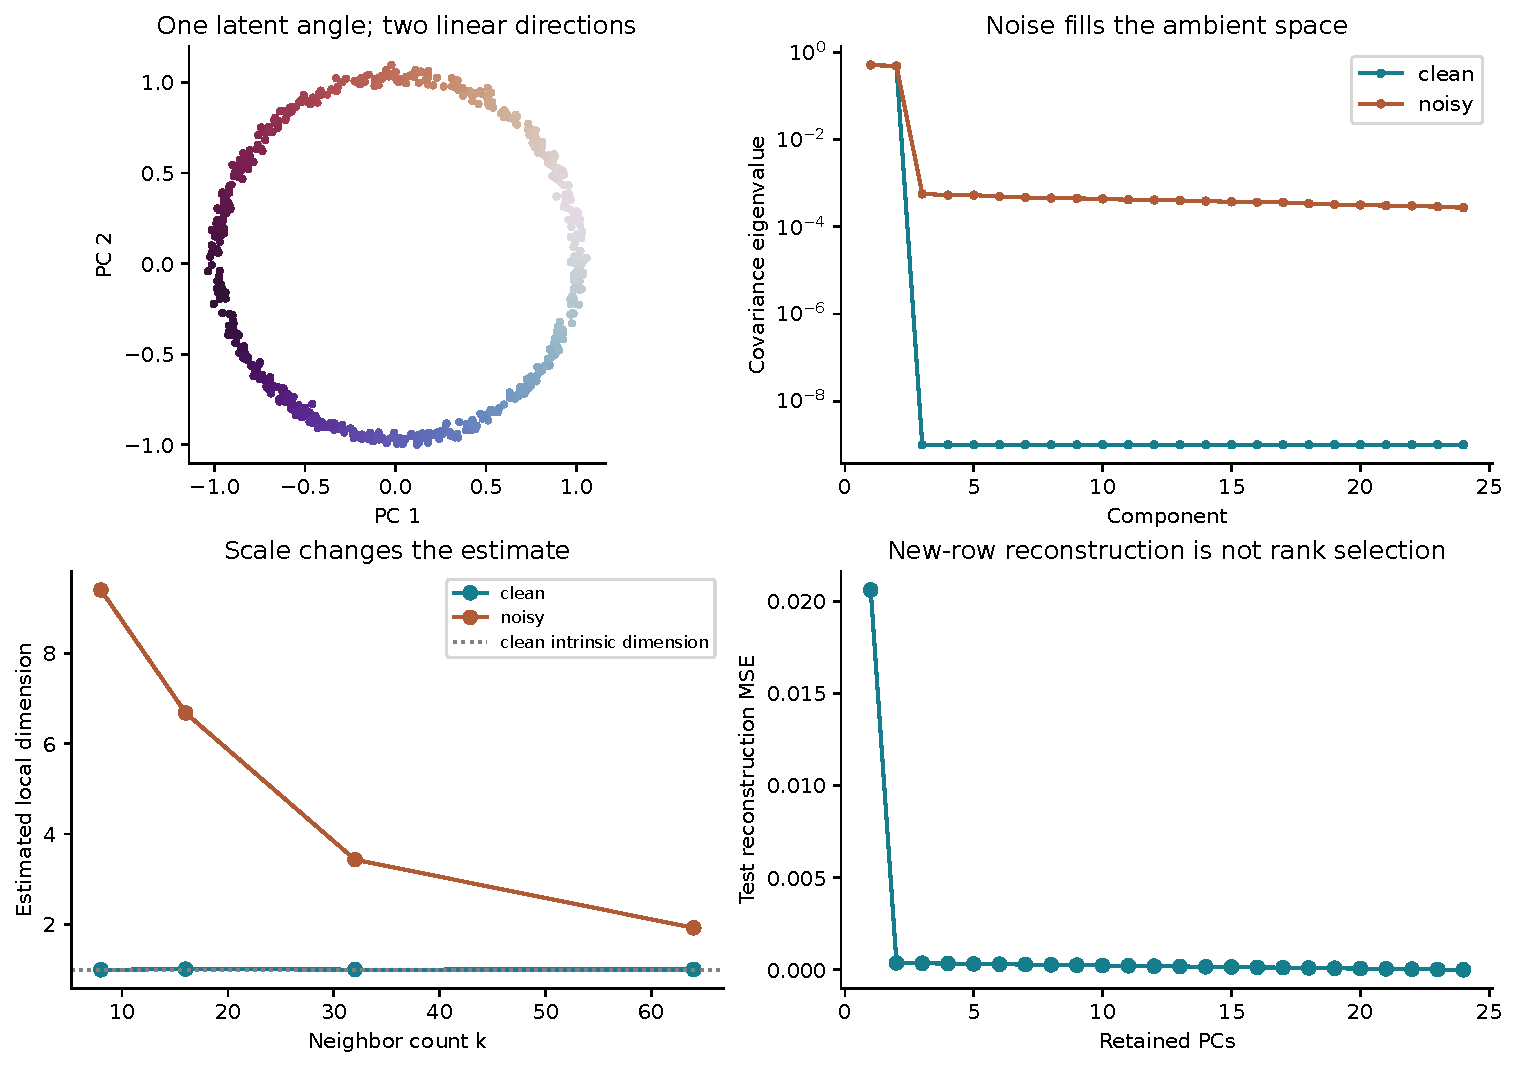
\includegraphics[width=\linewidth]{figures/pca_geometry.pdf}
\caption{Tutorial 1, synthetic data. Color in the upper-left panel denotes the known latent angle. The clean circle has one intrinsic coordinate and two linear directions. The spectra show observation noise beyond the first two components. The lower-left estimates change with neighborhood scale; the lower-right error illustrates why a particular cross-validation target can remain monotone in dimension.}
\label{fig:tutorial-pca}
\end{figure}

Useful controls change noise amplitude, neuron count, sampling density, and the neighborhood range separately. Repeat the clean/noisy comparison after a declared rescaling of each feature. If the estimate changes, identify whether the target metric itself changed. Do not report the smallest estimate as the ``true'' dimension merely because it matches an expectation.

\section{Tutorial 2: comparing embeddings against known geometry}
\subsection{Question and construction}
When does a visually convincing embedding preserve intrinsic distances? A Swiss roll gives a tractable test. Draw $t\in[1.5\pi,4.5\pi]$ and $v\in[0,20]$ independently and uniformly, and map
\begin{equation}
(t,v)\longmapsto(t\cos t,v,t\sin t).
\end{equation}
There are 650 observations with small isotropic coordinate noise. The noiseless induced metric is
\begin{equation}
 ds^2=(1+t^2)\,dt^2+dv^2.
\end{equation}
Set $s(t)=\tfrac12[t\sqrt{1+t^2}+\operatorname{arsinh}(t)]$. Since $ds/dt=\sqrt{1+t^2}$, the coordinates $(s(t),v)$ flatten this rectangular surface isometrically. Their Euclidean distances give an exact ground-truth intrinsic distance for the noiseless surface. Using $t$ directly as a distance coordinate would be wrong.

\subsection{Algorithm and diagnostic quantities}
The script compares PCA, Isomap, and UMAP. Isomap uses a six-neighbor graph for the main display and checks that it is connected. It also runs a twelve-neighbor sensitivity comparison. UMAP uses fifteen neighbors, minimum-distance parameter $0.1$, and a fixed random seed. These settings are transparent demonstration choices, not universal defaults certified for biological recordings.

For sampled pairs, let $a_{ij}$ be intrinsic distance and $b_{ij}$ embedding distance. To remove arbitrary global scale, minimize $\sum_{ij}(c b_{ij}-a_{ij})^2$ over $c$. Differentiation gives
\begin{equation}
 c_* = \frac{\sum a_{ij}b_{ij}}{\sum b_{ij}^2},\qquad
 \operatorname{stress}=\frac{\sqrt{\sum(c_*b_{ij}-a_{ij})^2}}{\sqrt{\sum a_{ij}^2}}.
\end{equation}
Spearman correlation tests the ranking of pairwise distances. Trustworthiness at ten neighbors detects points made spuriously close by the embedding relative to the observed input metric; it does not by itself test intrinsic distance preservation. No single one of these metrics is a complete embedding assessment.

\subsection{Result, parameter sensitivity, and interpretation}
In the recorded example, PCA has scaled intrinsic stress about $0.565$. Six-neighbor Isomap has stress about $0.032$, whereas changing to twelve neighbors raises it to about $0.413$. UMAP has stress about $0.164$. These values characterize this constructed example. They do not establish a general algorithm ranking. A neighborhood graph can remain connected while acquiring harmful shortcuts across different folds; connectivity is a necessary diagnostic here, not a sufficient guarantee of geodesic accuracy.

\begin{figure}[tbp]
\centering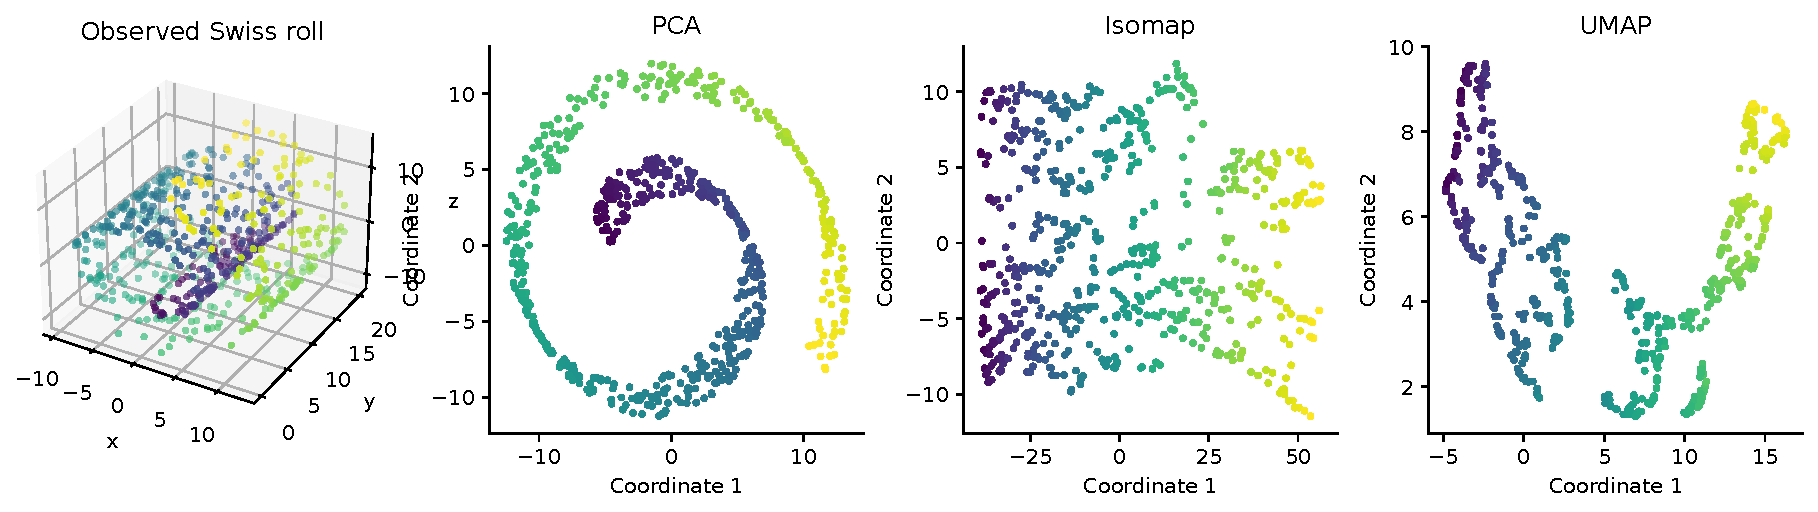
\includegraphics[width=\linewidth]{figures/embeddings.pdf}
\caption{Tutorial 2. All points are colored by the same generating spiral coordinate. PCA, six-neighbor Isomap, and UMAP are fitted to the same noisy Swiss roll. Ground-truth distance metrics and the twelve-neighbor Isomap sensitivity run are saved separately. A pleasing plot and a good local-neighborhood score do not certify global geometry.}
\label{fig:tutorial-embeddings}
\end{figure}

Because ground truth is available, the example can diagnose parameter sensitivity directly. Real experiments usually cannot tune against exact intrinsic distances. They should instead use independent measurements, a defensible generative model, stability across justified parameter ranges, and task-relevant predictions. Trying many settings and reporting only a persuasive ring or cluster is a form of analysis selection.

\section{Tutorial 3: phase portraits and numerical stability}
\subsection{Question, systems, and algorithm}
How do contraction, oscillation, and multiple basins differ? Three two-dimensional systems are simulated with adaptive numerical integration: a stable spiral, the Hopf normal-form oscillator, and a separable double well. The oscillator is
\begin{align}
\dot x&=(\mu-x^2-y^2)x-\omega y,\\
\dot y&=\omega x+(\mu-x^2-y^2)y.
\end{align}
The script compares $\mu=-0.3$ and $\mu=0.8$ with $\omega=1$. The double well uses $\dot x=x-x^3$, $\dot y=-2y$. These are dimensionless demonstration coordinates; they are not measured neural rates.

\lstinputlisting[language=Python,firstline=8,lastline=17,caption={The vector fields used for the phase-portrait examples.}]{code/03_phase_portraits.py}

\subsection{Expected and checked results}
For $\mu>0$, polar coordinates give $\dot r=\mu r-r^3$, so the stable cycle radius is $\sqrt{0.8}\simeq0.894427$. The largest final radius error among the simulated trajectories is below $10^{-8}$ in the recorded run. This comparison checks integration of a known solution property. The double-well trajectories approach either $(1,0)$ or $(-1,0)$ according to the sign of their initial $x$, while the separating stable manifold $x=0$ approaches the saddle at the origin.

\begin{figure}[tbp]
\centering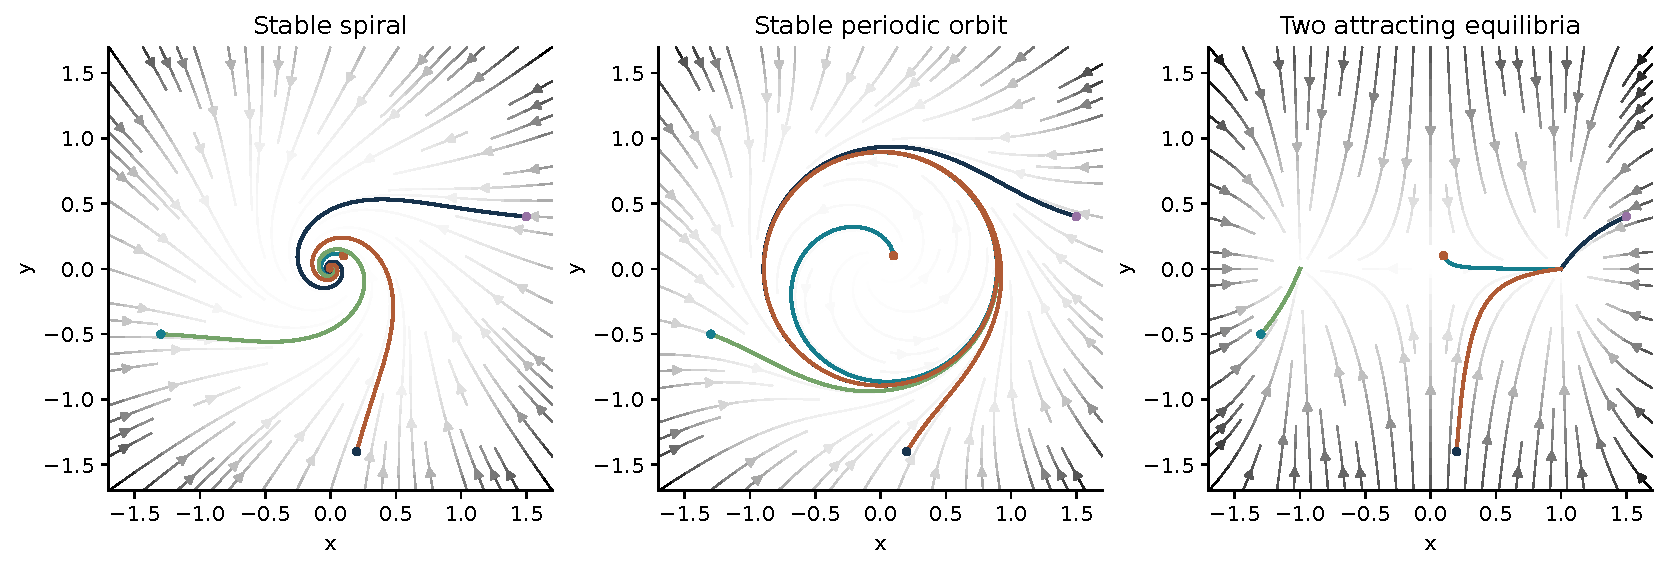
\includegraphics[width=\linewidth]{figures/phase_portraits.pdf}
\caption{Tutorial 3. Gray streamlines depict each vector field; colored curves are trajectories with marked initial states. A sink, a stable periodic orbit, and two attracting equilibria generate distinct phase portraits. Their appearances depend on retaining enough state variables.}
\label{fig:tutorial-phase}
\end{figure}

An additional sanity check contrasts exact evolution and Euler integration for $\dot x=-5x$ with step $\Delta t=0.5$. The exact multiplier is $e^{-2.5}\simeq0.0821$, whereas Euler gives $1-5\Delta t=-1.5$. Thus a numerically growing oscillation can be created by an unstable integration rule applied to a stable ODE. Reduce steps and compare methods before interpreting unexpected divergence. For an SDE, add noise with scale $\sqrt{\Delta t}$, not $\Delta t$; see Chapter~\ref{ch:02} and Appendix~\ref{app:d}.

\section{Tutorial 4: fixed points, residuals, and Jacobians}
\subsection{Question and mathematical model}
Does finding a near-stationary state establish stability? Consider
\begin{equation}
\dot h=-h+W\tanh h,\qquad
W=\diag(1.5,0.7),\qquad h\in\R^2.
\end{equation}
The activation acts before the recurrent matrix in this example. Consequently
\begin{equation}
J(h)=-I+W\diag(1-\tanh^2 h).
\end{equation}
This ordering differs from the equally legitimate model $\dot h=-h+\tanh(Wh)$; copying a Jacobian across the two conventions would be an error.

\subsection{Algorithm and results}
The script starts a numerical root solver from 70 states, checks $\norm{f(h_*)}<10^{-9}$, and merges candidates within $10^{-5}$. It finds approximately $(-1.287839,0)$, $(0,0)$, and $(1.287839,0)$. At the outer roots, the Jacobian eigenvalues are approximately $-0.605687$ and $-0.3$. At the origin they are $0.5$ and $-0.3$. The outer states are locally asymptotically stable; the origin is a saddle.

An independent central-difference calculation checks the analytical Jacobian. With $e_j$ a standard coordinate vector,
\begin{equation}
J_{\cdot j}(h)\approx\frac{f(h+\delta e_j)-f(h-\delta e_j)}{2\delta},
\qquad \delta=10^{-6}.
\end{equation}
Agreement to a declared tolerance detects indexing and derivative mistakes. It does not prove a model is scientifically appropriate.

\begin{figure}[tbp]
\centering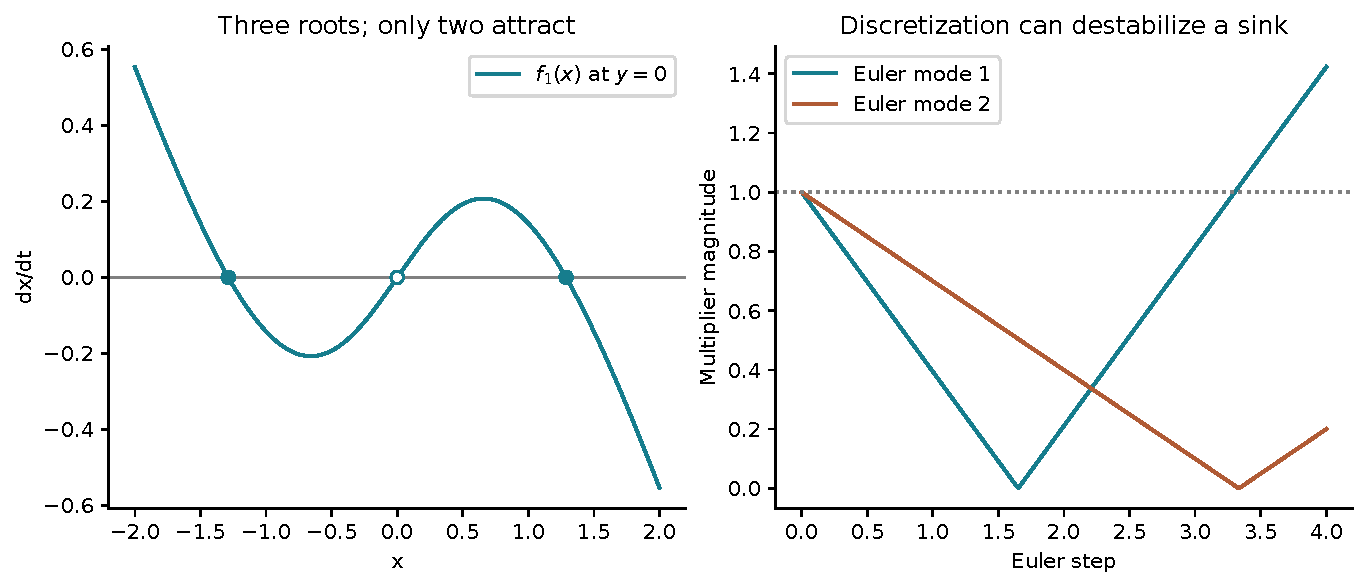
\includegraphics[width=0.96\linewidth]{figures/fixed_points.pdf}
\caption{Tutorial 4. Filled roots are stable in the continuous model and the unfilled root is unstable. The right panel shows magnitudes of the Euler multipliers at an outer equilibrium. Increasing the numerical step eventually destabilizes the discrete approximation even though the ODE remains stable.}
\end{figure}

Multistart search cannot certify that every root has been found. In this particular separable example, additional analytic reasoning can establish the count, but the generic search procedure does not do so. For trained networks, report initialization coverage, residual distributions, deduplication tolerances, and input conditions. Root stability is local; basin size requires further perturbations.

\section{Tutorial 5: a finite ring network and two kinds of perturbation}
\subsection{Question and construction}
What distinguishes attraction toward a family of states from attraction toward one particular state? Place $N=96$ model neurons at preferred angles $\theta_i=2\pi i/N$ and define
\begin{equation}\label{eq:tutorial-ring-rate}
\tau\dot r_i=-r_i+\sigma\!\left(\sum_j W_{ij}r_j\right),\quad
W_{ij}=\frac{-4+14\cos(\theta_i-\theta_j)}{N},\quad
\sigma(a)=\frac{1}{1+e^{-a}},\quad\tau=0.1\,\mathrm{s}.
\end{equation}
Rates are dimensionless and bounded. Euler integration uses $\Delta t=0.002\,\mathrm{s}$. A localized initial activity pattern relaxes to a stationary bump. The example probes an intentionally structured circuit; it does not learn this connectivity from neural data.

\subsection{Algorithm and perturbations}
First equilibrate the network, then restart from the same state for two interventions. At $3\,\mathrm{s}$, the radial intervention replaces $r$ with $0.6r+0.4\bar r\mathbf1$, reducing bump contrast. The phase intervention circularly shifts neuron rates by twelve indices. Track the complex first harmonic
\begin{equation}
 m(t)=\frac1N\sum_j r_j(t)e^{i\theta_j}.
\end{equation}
Its magnitude measures bump contrast and its argument measures phase when the magnitude is nonzero. A low magnitude would make phase estimates ill-conditioned.

The linearization is
\begin{equation}
J=\tau^{-1}\left[-I+\diag\{\sigma'(Wr_*)\}W\right].
\end{equation}
The recorded dimensionless stationary-map residual $\norm{-r_*+\sigma(Wr_*)}$ is below $2\times10^{-14}$; the ODE velocity residual is this quantity divided by $\tau$. The leading numerical eigenvalue is indistinguishable from zero at ordinary floating-point precision, while the next is approximately $-4.844\,\mathrm{s}^{-1}$. This indicates near-neutral phase motion and rapid contraction in another direction in this model.

\begin{figure}[tbp]
\centering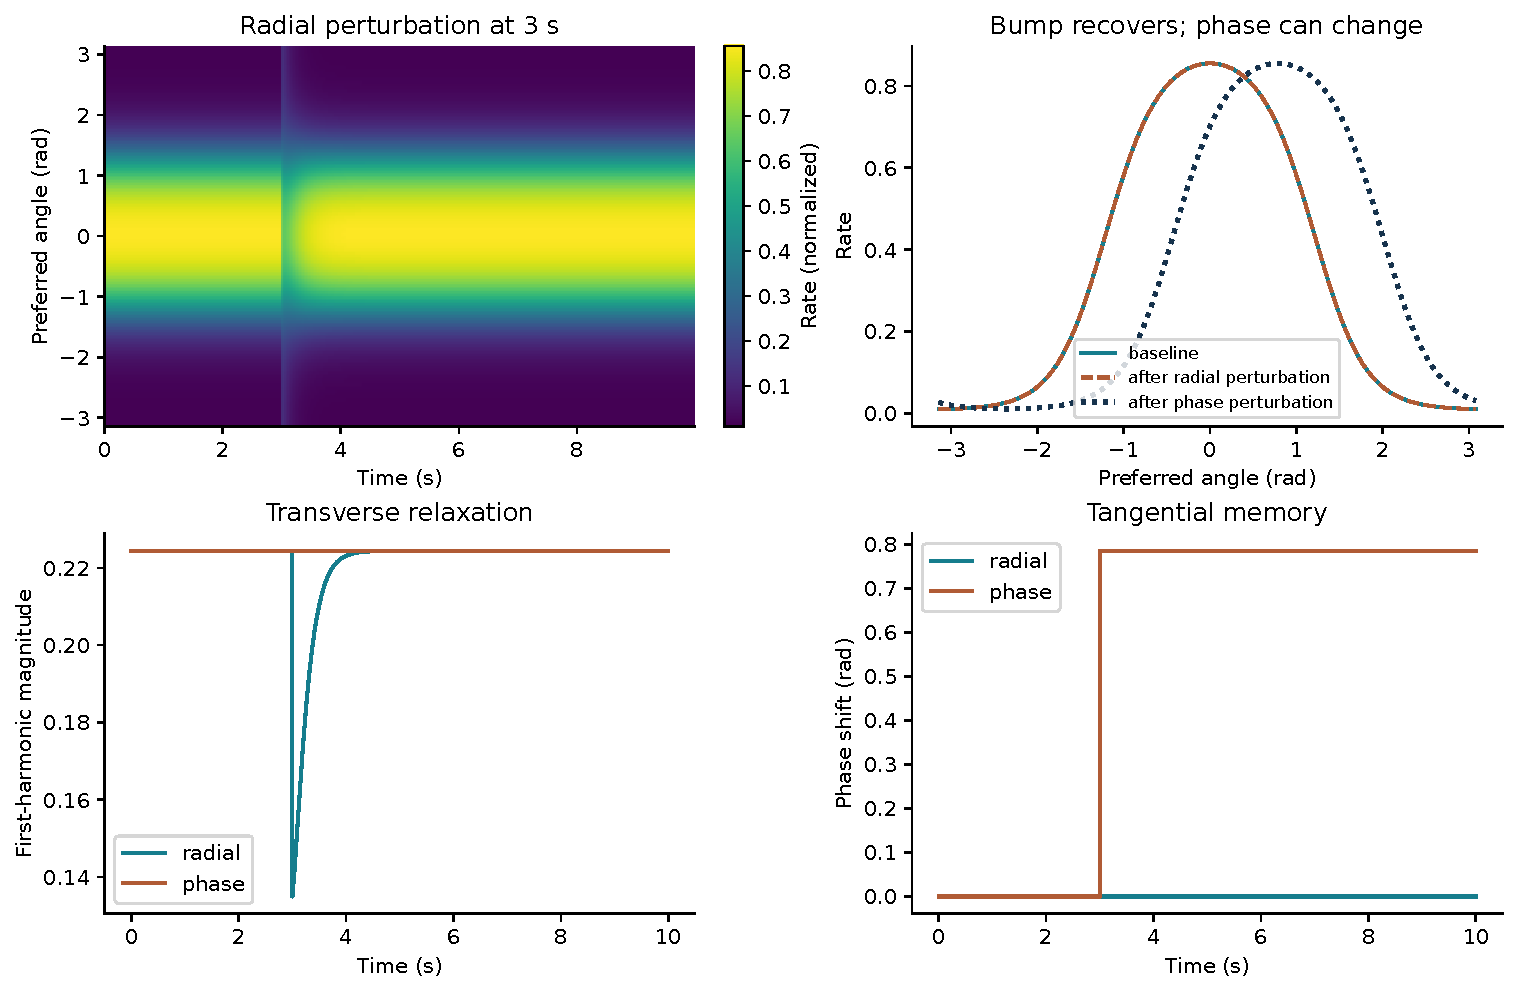
\includegraphics[width=\linewidth]{figures/ring_attractor.pdf}
\caption{Tutorial 5. The heat map and rate profiles show a localized bump. Reducing its contrast is followed by recovery. A phase shift remains, approximately $\pi/4$ for the twelve-neuron shift. The magnitude and phase panels separate transverse relaxation from motion along the represented family.}
\label{fig:tutorial-ring}
\end{figure}

\subsection{Interpretation and limits}
The finite network has exact discrete rotation symmetry, not exact symmetry under every real-valued angle. Very weak pinning can therefore be present even when a computed eigenvalue is nearly zero. Report the numerical tolerance and observation duration. Add heterogeneity, noise, or longer simulations to test robustness. A ring-shaped cloud alone could not establish the transverse relaxation seen in the intervention. Conversely, returning after the radial perturbation does not establish that phase is restored: the phase shift shows why set attraction and point attraction must be distinguished.

\section{Tutorial 6: a circle, sphere, torus, and disk}
\subsection{Question and data}
Can the same pipeline distinguish a prominent loop from a surface cycle, while revealing short-lived holes in a control? The script generates a noisy circle in $\R^2$, a sphere in $\R^3$, a product torus in $\R^4$, and points uniformly distributed across a filled disk. The torus uses
\begin{equation}
(\alpha,\beta)\longmapsto
(\cos\alpha,\sin\alpha,\cos\beta,\sin\beta),
\end{equation}
with a perturbed $14\times14$ angular grid. This is an embedded flat torus. It is different metrically from a doughnut surface in $\R^3$, although both have topology $T^2$. The sphere is generated by normalizing independent Gaussian vectors, which yields uniform directions before noise is added. Disk radii use $r=\sqrt U$ with $U$ uniform; choosing radius uniformly would oversample the center relative to area.

\subsection{Computation and interpretation}
Ripser computes $H_0$, $H_1$, and $H_2$ over $\F_2$ up to maximum edge length $2.3$ \citep{root_ripser}. The noiseless topological targets are $(\beta_0,\beta_1,\beta_2)=(1,1,0)$ for a circle, $(1,0,1)$ for a sphere, $(1,2,1)$ for a torus, and $(1,0,0)$ for a disk. A finite Rips filtration need not display these values at every scale. The diagram records classes of its complexes, not a direct certificate of the continuum object's identity.

\begin{figure}[tbp]
\centering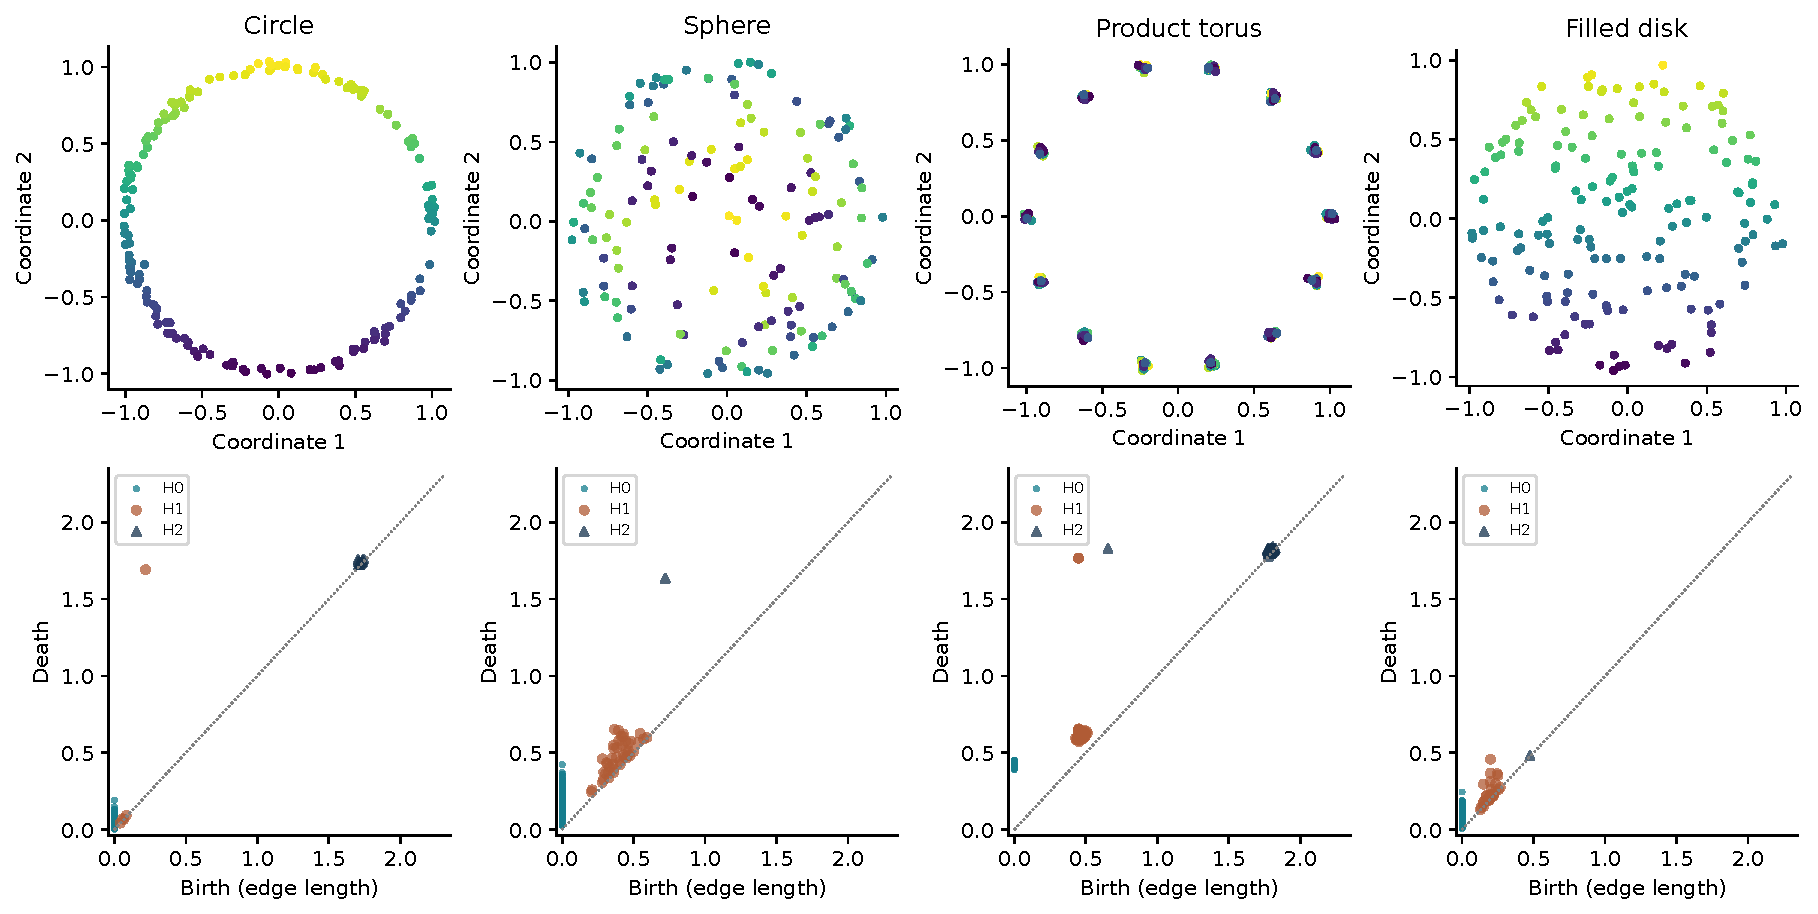
\includegraphics[width=\linewidth]{figures/topology_clouds.pdf}
\caption{Tutorial 6. The upper row shows only the first two observation coordinates; persistence is computed in each dataset's full ambient space. In particular, the torus projection discards an entire circular factor. The lower row shows finite persistence pairs for $H_0$ (dots), $H_1$ (circles), and $H_2$ (triangles). The essential $H_0$ class is omitted from the plotted finite pairs and retained in the saved arrays.}
\label{fig:tutorial-clouds}
\end{figure}

The sphere and torus exhibit long-lived $H_2$ features in this run, while the disk has shorter accidental holes. Even the circle can show small higher-dimensional Rips features at larger scales. A Rips complex is not always a faithful triangulation of the underlying manifold. Inspect intervals jointly, specify the scale range, and compare with appropriate noise and sampling controls. An infinite death time in a truncated calculation can mean a feature has not yet died by the last computed scale; do not automatically call it mathematically essential.

\section{Tutorial 7: a complete neural topological pipeline}
\subsection{Question and observation model}
Can coordinated angular tuning produce a statistically distinguishable loop in held-out population activity? For each of 24 model neurons, place a preferred angle $\phi_j$ evenly on the circle and define a measured rate
\begin{equation}
Y_{ij}=2+4\exp\{2[\cos(\theta_i-\phi_j)-1]\}+\eta_{ij},
\quad\eta_{ij}\sim\mathcal N(0,0.15^2).
\end{equation}
These are continuous noisy rate observations, not Poisson spike counts. Angles are sampled independently. Generate 500 training rows and 180 independent test rows. Fit eight-component PCA only on training data and transform the test rows with this frozen transformation. No label or persistence result is used to select the PCA basis.

\subsection{The statistic and the null}
Compute the test Rips diagram in eight PCA coordinates and define the statistic
\begin{equation}
T=\max_{(b,d)\in D_1,\ d<\infty}(d-b),
\end{equation}
with $T=0$ if no finite $H_1$ class exists. This maximum incorporates selection of the most persistent observed loop. The chosen null is independence between neuron columns across identically distributed independent test observations. Independently permute each raw test column, apply the same frozen PCA transformation, and recompute $T$ for 99 surrogates. Under the stated exchangeability null, the plus-one randomization value is
\begin{equation}
\widehat p=\frac{1+\#\{b:T_b\geq T_{\mathrm{observed}}\}}{100}.
\end{equation}
The minimum attainable value is $0.01$, which is not a statement that the true tail probability equals $0.01$. Selecting preprocessing or a statistic after viewing the test result would require nesting that selection in the null procedure or using additional independent data.

\subsection{Executable core}
The following excerpt includes the generating model, held-out preprocessing, and randomization loop. The full script adds figures and saves all arrays.
\lstinputlisting[language=Python,firstline=9,lastline=31,caption={The central steps of the neural persistence tutorial.}]{code/07_neural_persistence.py}

\subsection{Recorded result, checks, and limits}
The observed maximum $H_1$ lifetime is approximately $9.1655$ in PCA coordinates; the longest among the 99 null maxima is approximately $1.3168$, giving the attainable minimum $\widehat p=0.01$. Computing in the original 24-dimensional observation space also yields a long feature, about $8.9816$. These lifetimes have distance units in their respective spaces and are not universal effect sizes.

\begin{figure}[tbp]
\centering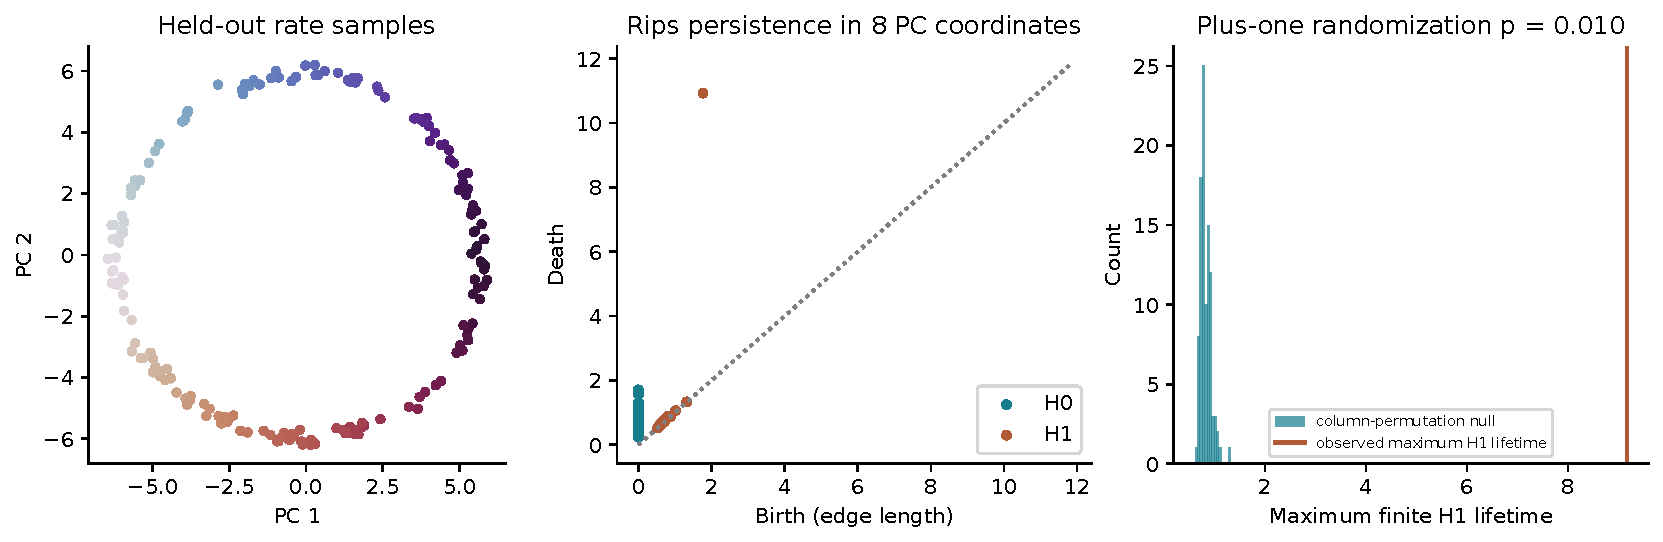
\includegraphics[width=\linewidth]{figures/persistence.pdf}
\caption{Tutorial 7. Left: the first two PCs of held-out observations, colored by generating angle. Middle: the persistence diagram computed using all eight retained PCs. Right: the null distribution of the prespecified maximum $H_1$ lifetime, with the observed statistic marked separately. The analysis establishes incompatibility with the specified independence null, not proof of a recurrent attractor.}
\label{fig:tutorial-persistence}
\end{figure}

The null destroys coordinated population tuning while preserving each neuron's empirical marginal distribution. It does not preserve a behavioral common input, and therefore cannot distinguish a feedforward angular code from an internally generated ring representation. The sampling is independent by construction. Applying this row-permutation scheme to temporally correlated neural recordings would generally be inappropriate. Trial-wise shuffles, circular time shifts, conditional surrogates, or explicit generative nulls answer different questions and require their own exchangeability or modeling assumptions. Chapter~\ref{ch:09} explains the corresponding experimental pipeline.

\section{Tutorial 8: hidden dynamics of a trained recurrent network}
\subsection{Question, task, and training}
Does a trained network solve delayed binary memory with stable states, or only with finite-duration transients? Train a 16-unit tanh RNN on cues of sign $s\in\{-1,+1\}$. Input is present for the first three steps and zero afterward. Cue strengths vary uniformly from $0.8$ to $1.2$ during training. A linear readout predicts the cue sign during the subsequent delay. The training sequence has 35 steps, minibatches have 64 trials, and Adam performs 650 updates. The loss is mean squared prediction error over delay steps.

The recurrent update is
\begin{equation}
h_{t+1}=\tanh(W_hh_t+W_uu_t+b),\qquad
\widehat s_t=w_o^Th_t+b_o.
\end{equation}
The included PyTorch implementation initializes the recurrent matrix orthogonally, clips gradient norm at one, uses double precision, and records the seed and optimizer state. These are training choices, not biological assumptions. The tested API and recurrent-state conventions are documented by PyTorch \citep{root_torch_rnn,app_torchlstm}.

\subsection{Separating training, projection, and dynamical analysis}
After training, freeze all parameters. Probe independent cue strengths from $0.7$ to $1.3$ for 150 steps. Fit PCA on a separate deterministic bank of training-range probe trajectories and project the test states through that same basis. The projection is descriptive. Roots and eigenvalues are computed in the full 16-dimensional state with input fixed at zero:
\begin{equation}
F(h)=\tanh(W_hh+b),\qquad
F(h_*)-h_*=0,\qquad
DF(h_*)=\diag[1-F(h_*)^2]W_h.
\end{equation}
Local stability requires $\rho(DF)<1$. Here the eigenvalues are dimensionless multipliers per recurrent step, not continuous-time rates.

Root searches start from sampled delay states, random states, and zero. Accepted roots have residual below $10^{-8}$; nearby candidates are merged. The script checks the formula for $DF$ against automatic differentiation. For GRUs and LSTMs, the companion utility uses the actual cell implementation, including all gating derivatives. An LSTM state is the concatenation $(h,c)$:
\lstinputlisting[language=Python,firstline=10,lastline=24,caption={Automatic differentiation of the complete recurrent state.}]{code/recurrent_tools.py}
A hidden-only LSTM Jacobian would omit dynamically relevant cell-state directions. The script validates full-state dimensions for a small GRU and LSTM, but the trained demonstration is a tanh RNN; it does not claim to have trained all three architectures.

\subsection{Recorded result and evidential scope}
The recorded seed achieves $100\%$ cue-sign accuracy at step 35 on the test bank. Its mean squared readout error is approximately $1.79\times10^{-8}$ at both steps 35 and 150. The search finds two locally stable roots with spectral radii approximately $0.6211$ and $0.5231$, whose readouts are near $-1$ and $+1$, plus an unstable root with spectral radius approximately $1.7448$. These results support a bistable memory account for this trained instance under zero input.

\begin{figure}[tbp]
\centering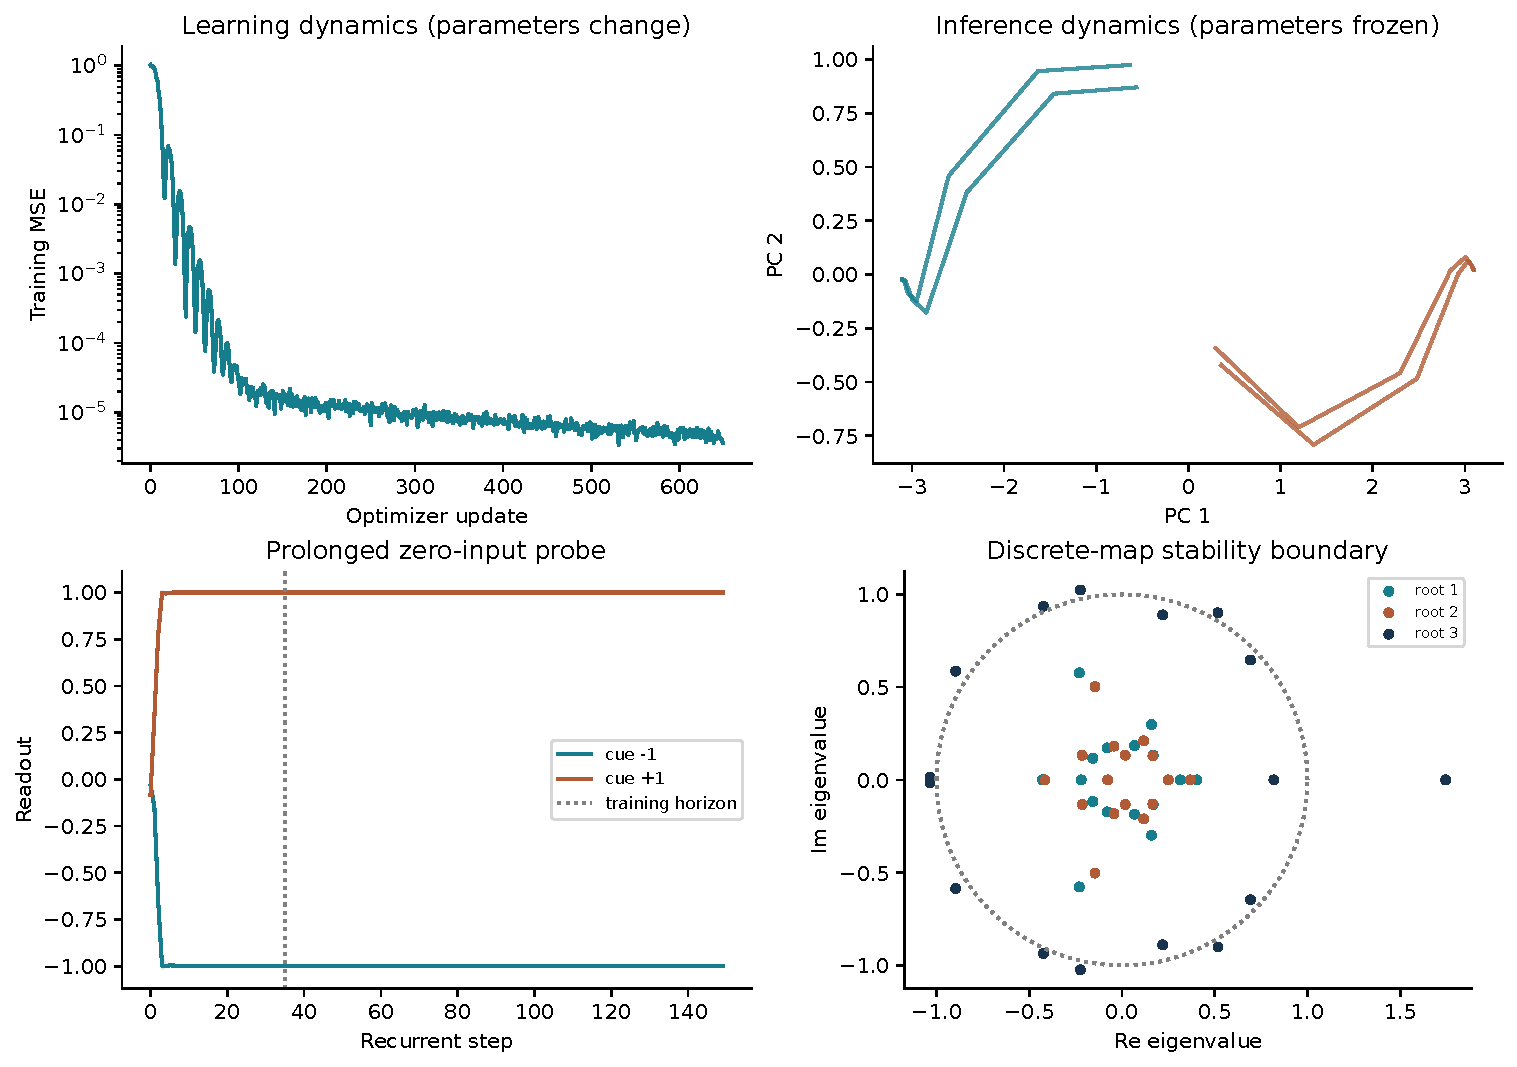
\includegraphics[width=\linewidth]{figures/rnn_dynamics.pdf}
\caption{Tutorial 8. Training loss indexes optimizer updates; hidden trajectories index inference steps after parameters have been frozen. Blue and orange trajectories represent negative and positive cues. The prolonged-delay readout extends beyond the training horizon. The eigenvalue plot compares roots with the discrete-time unit circle; the search is not certified globally complete.}
\label{fig:tutorial-rnn}
\end{figure}

A stronger mechanistic analysis would perturb each candidate root along multiple directions, map basin changes as inputs vary, repeat training across seeds, and test whether the readout uses the predicted state coordinates. The current root search cannot establish that no other equilibria or recurrent structures exist. Successful delayed memory in a different RNN could be transient, input-supported, or distributed across more complicated structures. The checkpoint and probe arrays permit those extensions without retraining this example.

\section{Tutorial 9: identical observations, different mechanisms}
\subsection{A controlled nonidentifiability example}
Suppose the recorded trajectory is exactly $x_0(t)=(\cos t,\sin t)$. Compare two systems:
\begin{align}
\text{Recurrent:}\quad\dot x&=(1-\norm{x}^2)x+Rx,
& R&=\begin{bmatrix}0&-1\\1&0\end{bmatrix},\\
\text{Externally driven:}\quad\dot x&=(-\sin t,\cos t).
\end{align}
Both start at $(1,0)$. The recurrent system has transverse radial contraction toward its unit limit cycle. The second integrates a supplied clock-dependent velocity; its current state does not regulate that velocity. Their unperturbed trajectories, PCA plots, and point-cloud topology coincide. A topology calculation alone therefore cannot distinguish them.

\subsection{Intervention and explicit hypothesis test}
Add the same radial displacement $\delta=0.3$ at the start of each system. In the recurrent system, $\dot r=(1-r^2)r$ restores radius one. In the driven system, the displacement persists as a constant vector offset from the reference path. After one full cycle, compare the signed radial displacement $\norm{x}-1$. Add independent Gaussian observation noise with coordinate standard deviation $0.03$ to 200 repeated observations per model. The prespecified statistic is the difference of group mean radial displacements. A 999-permutation comparison tests equality of the two observation distributions under exchangeability.

\begin{figure}[tbp]
\centering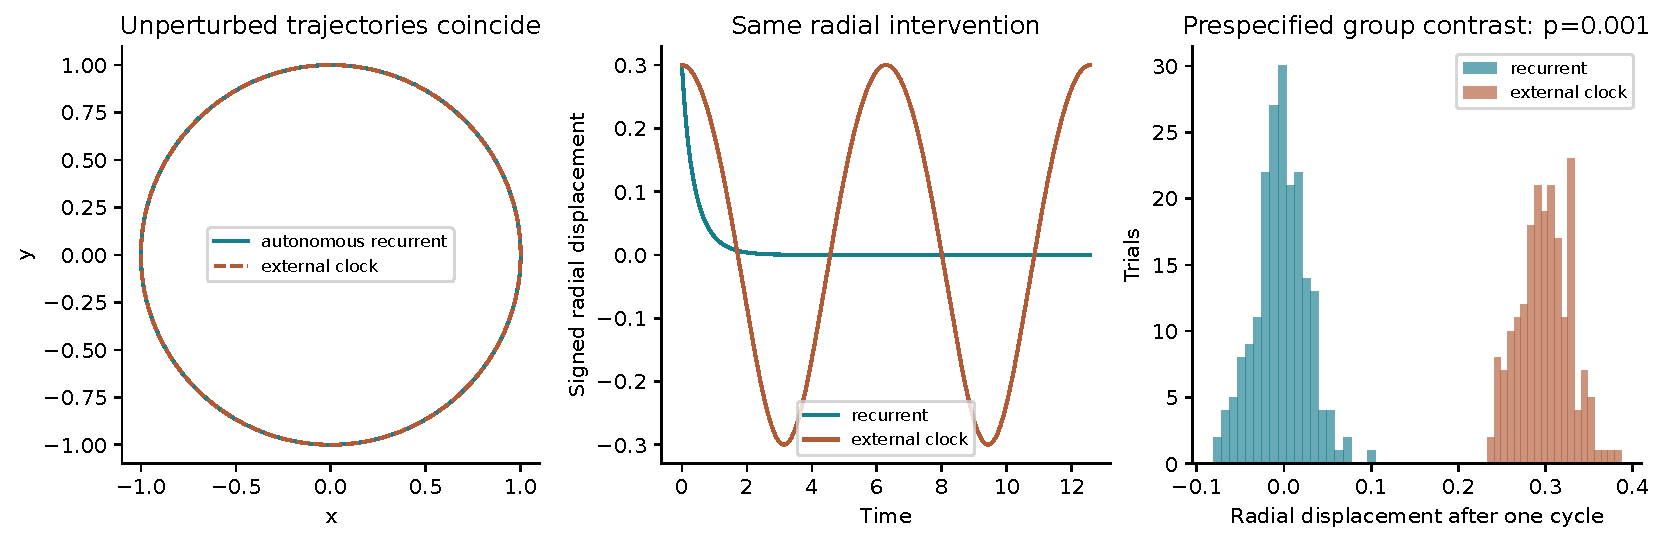
\includegraphics[width=\linewidth]{figures/null_hypotheses.pdf}
\caption{Tutorial 9. The unperturbed trajectories agree to numerical integration precision. A matched radial intervention separates the models. The last panel shows repeated noisy measurements after one complete cycle. The permutation test concerns this declared intervention contrast, not the probability that a model is true.}
\label{fig:tutorial-null}
\end{figure}

The unperturbed numerical discrepancy is below $2\times10^{-10}$ in the recorded run. The intervention mean contrast is about $0.302$ and the plus-one permutation value is $0.001$, the smallest attainable with 999 surrogates. This distinguishes these two specified mechanisms. An externally driven system with feedback could also restore perturbations, so the result would not isolate an entirely internal biological generator without measuring or manipulating the relevant inputs. Chapter~\ref{ch:12} expands this identifiability argument.

\section{What to report when transferring these tools to real data}
A reproducible report should identify the sampling unit, trial structure, preprocessing fitted on each split, observation metric, model state, input condition, estimator, and uncertainty target. For topology, include coefficient field, filtration convention, scale truncation, landmark selection if any, and the statistic used in the null comparison. For dynamics, include time units, differentiation or integration method, fixed-point residuals, Jacobian convention, search initialization, and perturbation sizes. The question is whether another analyst could reproduce both the result and the inference made from it.

There is no single validation protocol that covers every claim. A latent model used to predict firing rates needs held-out prediction assessment. A proposed circular representation needs evidence for periodic structure and appropriate topological or decoding controls. A proposed attractor needs evidence for dynamics toward an invariant set under declared input conditions. A proposed mechanism needs discriminating predictions or interventions. Matching the validation to the claim is the main lesson shared by the tutorials.

\section{Exercises}
\begin{enumerate}
\item \textbf{Introductory.} In Tutorial 1, remove observation noise. Explain why retaining two PCs reconstructs the data exactly although intrinsic dimension is one.
\item \textbf{Introductory.} For Tutorial 4, compute the discrete Euler multipliers at step $\Delta t=4$. Explain why the resulting numerical instability does not change the ODE's local stability.
\item \textbf{Intermediate.} Repeat Tutorial 2 with several neighborhood counts. Record graph connectivity, intrinsic stress, and local trustworthiness before looking at the plots. Can two metrics disagree?
\item \textbf{Intermediate.} Replace the twelve-neuron phase shift in Tutorial 5 with interpolation by half a neuron. Test long-duration drift and explain how finite sampling breaks an ideal symmetry.
\item \textbf{Intermediate.} In Tutorial 7, replace independent angular samples with a slowly varying trajectory. Explain why individual row permutations become an inadequate temporal null, and specify what a new surrogate should preserve.
\item \textbf{Intermediate.} Verify that collapsing the second circular factor in Tutorial 6's torus projection changes what can be identified from two plotted coordinates.
\item \textbf{Advanced.} Train Tutorial 8 across at least five seeds, with shorter training delays and wider test delays. Compare task accuracy, root spectra, and perturbation return. State how you will handle unsuccessful training runs before seeing results.
\item \textbf{Advanced.} Modify the driven model in Tutorial 9 to add feedback from $x-x_0(t)$. Can it now mimic the recurrent perturbation response? Propose a further intervention that distinguishes the new competing models.
\end{enumerate}

\section{Summary and further reading}
These tutorials connect models, observations, statistics, and discriminating controls. Synthetic results validate the declared examples, not biological mechanisms. For method references, see Chapters~\ref{ch:01}, \ref{ch:04}, \ref{ch:06}, and \ref{ch:10}; consult the cited software documentation for implementation details.

\part{Critical analysis of the research literature}
\chapter{What Mathematical Claims Can Neural Data Support?}\label{ch:12}

\section*{Learning objectives}
By the end of this chapter, the reader should be able to separate a mathematical object from its estimator, formulate an empirical claim with an explicit scope, identify observationally indistinguishable mechanisms, and design controls that address a particular alternative explanation. The aim is neither to prohibit useful approximations nor to demand an impossible proof from an experiment. It is to make the chain from observation to interpretation inspectable.

\section{One picture, several scientific claims}
Imagine that a two-dimensional display of population activity shows a ring. There are at least five different possible statements:
\begin{enumerate}
\item This particular embedding contains a visible hole.
\item The chosen metric on the measured activity has a persistent one-dimensional homology class.
\item The observations are noisy samples near a smooth one-dimensional closed manifold.
\item The relevant neural state evolves near an invariant, attracting circle.
\item Recurrent connections within the recorded circuit generate and maintain that circle.
\end{enumerate}
Each statement concerns a different object. An embedding is the output of an algorithm; persistent homology describes a filtration built from distances; a manifold is a local geometric structure; attraction is a property of a time-evolution rule; a circuit mechanism concerns causal interactions. None of these distinctions diminishes the value of a ring visualization. They identify the additional work required to move from one claim to the next.

Throughout, let the underlying state be \(x_t\), the measured response be
\begin{equation}\label{eq:12-observation}
y_t=g(x_t)+\varepsilon_t,
\end{equation}
and the processed response be \(\widetilde y_t=P(y_{1:T})_t\). Here \(g\) is the observation map, \(\varepsilon_t\) is measurement noise, and \(P\) includes binning, smoothing, normalization, neuron selection, and dimensionality reduction. A conclusion about \(\widetilde y\) is not automatically a conclusion about \(x\). In particular, smoothing may use neighboring times, and a projection may identify distinct states.

\section{A six-part statement of a claim}\label{sec:12-framework}
For any substantive claim, write the following six elements before selecting the analysis.
\begin{description}
\item[A. Mathematical definition.] Specify the object and the ambient setting. For example: a compact attracting invariant set of a specified autonomous flow, or a \(d\)-dimensional smooth embedded manifold.
\item[B. Operational definition.] State the finite-data criterion. For example: the first \(k\) principal components explain a specified fraction of held-out variance, or an estimated transverse drift is negative over a prespecified range.
\item[C. Empirical evidence.] Identify the observations and the statistic, including the population, behavioral regime, recording duration, preprocessing, and uncertainty.
\item[D. Strength of inference.] State the narrowest claim that the evidence supports. An estimator can support a model assumption without verifying every hypothesis of a theorem.
\item[E. Alternative explanations.] Give at least one explicit competing data-generating process, not merely the word \emph{noise}.
\item[F. Stronger validation.] Specify a new observation, held-out prediction, or perturbation on which the competing explanations disagree.
\end{description}
This structure separates disagreements about definitions from disagreements about evidence. A linear factor model may legitimately call its fitted subspace an operational neural manifold. The scientific question is whether subsequent conclusions require only that subspace or silently require curvature, topology, or attraction.

\begin{example}[A claim about dimensionality]
Suppose a model with five latent variables predicts unobserved neurons better than models with two or ten variables. A defensible statement is that five dimensions give the best predictive trade-off among the tested models, for these neurons, trials, and recording conditions. This is not the assertion that the complete circuit has exactly five dynamical degrees of freedom. A different observation map, stimulus distribution, noise model, or time resolution could change the predictive optimum.
\end{example}

\section{Why finite samples do not certify a manifold}
A finite point cloud, equipped with its subspace topology from Euclidean space, is discrete: each distinct point has a sufficiently small neighborhood containing no other sampled point. The cloud is therefore not literally the continuous circle or surface that an analysis seeks to infer. The scientific object is a hypothesized support, latent state space, or concentration set of a sampling distribution.

\begin{proposition}[An exact fit does not identify dimension]\label{prop:12-interpolation}
For any finite set of distinct points in \(\R^p\), with \(p\geq 2\), there is a smooth embedded one-dimensional manifold containing every point. The same point set is also contained in the \(p\)-dimensional manifold \(\R^p\).
\end{proposition}
\begin{proof}
Choose a direction \(a\) such that \(a^\top(x_i-x_j)\ne0\) for every distinct pair. Such a direction exists because the finitely many forbidden hyperplanes cannot cover \(\R^p\). After an orthogonal change of coordinates, write the points as \((t_i,z_i)\), with all \(t_i\) distinct and \(z_i\in\R^{p-1}\). For each coordinate of \(z\), polynomial interpolation gives a polynomial \(q_j(t)\) with \(q_j(t_i)=(z_i)_j\). The graph
\[
\Gamma=\{(t,q_1(t),\ldots,q_{p-1}(t)):t\in\R\}
\]
contains the sample. Its parametrization is injective, its derivative has first component one, and projection onto the first coordinate is a continuous inverse. Hence it is a smooth embedding of \(\R\).
\end{proof}
The construction may bend wildly between observations. Its purpose is not to recommend interpolation; it proves why an assumption about regularity and sampling is unavoidable. Generalization to new observations, bounded curvature, noise estimates, and coverage of the proposed support constrain the many possible interpolating geometries.

Manifold reconstruction theorems make such assumptions explicit. For example, the framework of \citet{ev_niyogi2008} controls geometric scale through a condition number related to curvature and near self-intersections and imposes sampling conditions. The existence of a recovery theorem is not evidence that its sampling and noise hypotheses hold in a particular recording.

\begin{insight}{A useful operational formulation}
Instead of saying that the data are a manifold, ask whether a specified distribution of observations concentrates near an approximately smooth \(d\)-dimensional set, at a stated spatial and temporal scale, with errors small enough for the scientific question. Then report the tests of that approximation.
\end{insight}

\section{A dictionary of definitions and measurements}
Table~\ref{tab:12-dictionary} collects recurring distinctions. Definitions are abbreviated here; Chapters~\ref{ch:01}--\ref{ch:05} provide the mathematical qualifications.

{\scriptsize
\setlength{\tabcolsep}{2pt}
\begin{longtable}{>{\raggedright\arraybackslash}p{.10\linewidth}>{\raggedright\arraybackslash}p{.18\linewidth}>{\raggedright\arraybackslash}p{.16\linewidth}>{\raggedright\arraybackslash}p{.17\linewidth}>{\raggedright\arraybackslash}p{.18\linewidth}>{\raggedright\arraybackslash}p{.13\linewidth}}
\caption{From formal terms to empirical measurements. A supported inference is conditional on the listed operational choice.}\label{tab:12-dictionary}\\
\toprule
Term & Formal definition & Common neuroscience usage & Typical measurement & What can be inferred & Common overinterpretation\\
\midrule
\endfirsthead
\toprule
Term & Formal definition & Common neuroscience usage & Typical measurement & What can be inferred & Common overinterpretation\\
\midrule
\endhead
\bottomrule
\endfoot
Linear dimension & Dimension of a vector subspace; rank of a matrix & Number of components explaining substantial response variance & Singular values; held-out reconstruction & Compressibility under the selected norm and distribution & Total circuit dimension is fixed by a PCA threshold\\
Intrinsic dimension & Local coordinate dimension of a manifold & Number of latent degrees of freedom at a chosen scale & Local PCA; neighbor-distance estimators; model comparison & Evidence for a local low-dimensional approximation & A precise, scale-independent biological integer\\
Effective dimension & A statistic of a spectrum, such as participation ratio & Breadth of population covariance & \((\sum_j\gamma_j)^2/\sum_j\gamma_j^2\) & Variance spread across orthogonal modes & Topological or manifold dimension\\
Manifold & Hausdorff, second-countable, locally Euclidean space; smooth compatibility when claimed & Restricted repertoire or fitted latent surface & Reconstruction, local dimension, out-of-sample prediction & Adequacy of a geometric model in sampled regions & Smoothness and global topology follow from a plot\\
Intrinsic geometry & Distances or metric tensor defined on the space itself & Neighborhood or geodesic relations of neural states & Graph distances; local metric estimates & Structure under the chosen metric and sampling scheme & Any nonlinear embedding preserves neural distances\\
Topology & Properties invariant under homeomorphism & Connected components and holes across scales & Persistent homology/cohomology & Homological features of the chosen filtration & Betti numbers uniquely identify the space\\
Attractor & Compact invariant, stable, locally attracting set under the convention used here & Frequently occupied or apparently recurrent activity state & Return trajectories; drift; perturbations; model basins & Evidence for attraction in the observed regime & High occupancy alone establishes attraction\\
Stability & Response to sufficiently small state perturbations over time & Reproducible signals or similar activity across days & Jacobian spectra; perturbation response; cross-session alignment & The particular kind of robustness that was measured & Reproducibility is Lyapunov stability\\
Repre\-sen\-ta\-tion & A specified map between variables and neural states or readouts & Information about a task variable in activity & Encoding, decoding, invariance, interventions & Predictive association, and causal use if separately tested & Decodability proves the circuit uses that variable\\
Latent dynamics & A transition rule on a latent state space & A fitted evolution model for observations & Forecasting; likelihood; residuals; interventions & A predictive dynamical description within tested conditions & The fitted coordinates are unique biological variables\\
\end{longtable}
}

\section{Geometry is not an autonomous mechanism}
\subsection{Identical trajectories with different attraction}
Consider the unit-circle trajectory
\[
y(t)=(\cos\omega t,\sin\omega t),\qquad \omega>0.
\]
It solves the linear system \(\dot y=\omega Jy\), where
\[
J=\begin{pmatrix}0&-1\\1&0\end{pmatrix}.
\]
Every circle is invariant, but the unit circle does not attract nearby radii: \(\frac{\dd}{\dd t}\norm{y}^2=0\). It also solves
\begin{equation}\label{eq:12-attracting-circle}
\dot y=(1-\norm{y}^2)y+\omega Jy.
\end{equation}
For this second system, \(r=\norm y\) obeys \(\dot r=r(1-r^2)\); the derivative of the radial drift at \(r=1\) is \(-2\). Small radial deviations decay. A third system can simply be an externally prescribed periodic input that drives two otherwise passive channels. On the displayed trajectory, all three agree.

Off-trajectory observations distinguish these explanations. A radial displacement produces neutral persistence in the first model, relaxation in the second, and an input-dependent response in the third. Consequently, longer observation of one unperturbed orbit need not resolve a mechanistic ambiguity. An intervention directed into a previously unvisited state-space direction may be much more informative.

\subsection{Projection can destroy closure}
Suppose
\[
\dot x_1=x_2,\qquad \dot x_2=-x_1,
\]
but only \(y=x_1\) is recorded. At \(y=0\), the derivative can be positive or negative, depending on unobserved \(x_2\). There is no single-valued autonomous rule \(\dot y=F(y)\) valid for all states. A fitted conditional mean drift may still exist, but it averages over hidden states rather than recovering a closed deterministic law.

A practical closure check asks whether histories, external inputs, or additional recorded variables improve prediction after conditioning on the proposed latent state. Failure to detect improvement is not proof of closure: the added measurements may be too noisy. Detectable improvement is direct evidence that the reduced state is insufficient for the proposed autonomous model.

\section{Attraction, noise, and apparent return}
\subsection{Occupancy does not determine drift}
A density describes where observations occur; dynamics also describes their directed transitions. For a diffusion
\[
\dd x_t=b(x_t)\,\dd t+\sqrt{2D}\,\dd W_t,
\]
the stationary density \(\rho\), when sufficiently regular, satisfies
\[
0=-\nabla\cdot(b\rho)+D\Delta\rho.
\]
Knowing \(\rho\) alone does not determine \(b\). Different probability currents \(b\rho-D\nabla\rho\) may have zero divergence and share the same density. An energy defined as \(-\log\rho\) is therefore not generally a physical potential whose negative gradient generates the drift. Such an identification requires additional assumptions, including the appropriate diffusion model and equilibrium or detailed-balance structure.

This is especially clear on a circle. Uniform occupancy is compatible with no deterministic angular drift, constant clockwise drift, or a sufficiently symmetric stochastic process. Conversely, nonuniform occupancy can arise from nonuniform behavioral sampling even if an internal angular coordinate has no preferred state.

\subsection{A worked measurement-noise counterexample}
Let a genuinely constant hidden state be observed as \(y_t=\mu+\varepsilon_t\), with independent, zero-mean measurement errors. Then
\begin{align}
\E[y_{t+1}-y_t\mid y_t]
&=\E[\mu+\varepsilon_{t+1}-y_t\mid y_t]\\
&=\mu-y_t.
\end{align}
A regression of measured displacement on measured displacement from the mean finds inward drift, although no hidden-state displacement occurred at all. The same observation error contributes positively to the regressor and negatively to the increment. This is a precise form of regression to the mean.

Temporal correlation changes the artifact without removing the issue. If the errors follow a stationary Gaussian autoregression with conditional mean \(\E[\varepsilon_{t+1}\mid\varepsilon_t]=\rho\varepsilon_t\), then the apparent slope is \(\rho-1\). Binning and filtering change this correlation. Therefore, apparent return should be compared with an observation-noise model that undergoes the same preprocessing.

\begin{insight}{Stronger evidence for attraction}
Estimate a candidate set from independent data; characterize noise; test return after a displacement whose size exceeds measurement uncertainty; examine several transverse directions; report return times and failures; and compare models with input-driven correction. When only passive recordings are available, state that transverse drift is observational evidence compatible with attraction rather than a complete causal identification of recurrence.
\end{insight}

\section{What a topological result does and does not identify}
A long-lived \(H_1\) class is evidence for a robust loop in a filtration, relative to its metric and scale. It does not distinguish a circle from an annulus, which has the same homotopy type, nor establish one-dimensional local neighborhoods. Betti numbers \((1,2,1)\) are compatible with a torus but also with the wedge \(S^1\vee S^1\vee S^2\), which is not a surface at the common attachment point. Over \(\F_2\), they also fail to distinguish a torus from a Klein bottle.

Additional assumptions can change the inference. A connected, compact, orientable, boundaryless two-dimensional manifold with first Betti number two is a torus by the classification of surfaces. The force of the conclusion comes from the \emph{combination} of the theorem and those assumptions. A persistence diagram does not itself establish them.

Persistent homology also leaves timing unspecified. Permuting the order of point-cloud samples preserves all pairwise distances and its ordinary persistence diagram. It can destroy every temporal trajectory while leaving the topological result unchanged. Thus a topological analysis can complement, but cannot substitute for, dynamical analysis.

\section{Null models should encode a scientific alternative}\label{sec:12-nulls}
The null hypothesis is not that nothing interesting happened. It is a family of processes that can account for specified properties without the additional mechanism being claimed. \citet{ev_elsayed2017} developed neural population controls that preserve selected simpler features while testing additional population structure. The general principle is to preserve what the alternative already explains.

Consider a loop statistic \(T\), such as the longest finite \(H_1\) lifetime. Different surrogates ask different questions:
\begin{itemize}
\item Independent time shuffles per neuron test whether temporal coordination matters, but also destroy autocorrelation and behavioral tuning relationships.
\item Independent circular shifts preserve each neuron's sequence up to a time origin; they usually disrupt simultaneous coordination. Their validity depends on stationarity and on whether wraparound is scientifically plausible.
\item Trial-label shuffles within a matched condition preserve condition means but alter trial-specific population dependence, provided trials are exchangeable within that condition.
\item A fitted behavior-driven encoding model asks whether tuning and the observed behavioral trajectory suffice to produce the statistic.
\item A fitted latent stochastic process asks whether covariance, smoothness, and sampling alone suffice.
\end{itemize}
Rejecting one null does not reject all alternatives. An independent-neuron null is an especially weak test of a recurrent attractor claim when coordinated external input is plausible.

For exchangeable observed and surrogate statistics \(T_{\mathrm{obs}},T_1,\ldots,T_B\), a Monte Carlo upper-tail value is
\begin{equation}\label{eq:12-montecarlo}
p=\frac{1+\sum_{b=1}^B\mathbf1\{T_b\geq T_{\mathrm{obs}}\}}{B+1}.
\end{equation}
The added one prevents an impossible report of zero and accounts for the observed dataset in the rank \citep{ev_phipson2010}. Exchangeability is the substantive requirement. Surrogates from a model fitted to the same data generally require a parametric-bootstrap interpretation, refitting, or calibration; the rank formula alone does not make them an exact test.

If preprocessing parameters were chosen to maximize \(T_{\mathrm{obs}}\), the identical search should be repeated inside each surrogate, or the final configuration should be evaluated on independent data. Otherwise the null distribution does not include the researcher's selection procedure. Reporting the entire sensitivity analysis is often more informative than reporting the most favorable parameter setting.

\section{Prediction, invariance, and intervention}
\subsection{Prediction has levels}
Reconstructing the points used to fit a model is the weakest prediction. Predicting withheld time bins from immediately adjacent smoothed bins may also be easy. More demanding tasks include predicting independent trials, unobserved neurons, new initial states, changed inputs, and responses to perturbations. These tests ask different questions; none is a universal ranking that ignores the scientific goal.

For temporal models, train-test splits should preserve the relevant unit of independence. If smoothing reaches across the split, a held-out value partly enters its own predictor. If several sessions share the same animal, uncertainty over time bins is not uncertainty over animals. Report both the statistical unit and the intended generalization population.

\subsection{Latent coordinates have a gauge freedom}
Suppose a state-space model uses \(z_{t+1}=F(z_t)\), \(y_t=g(z_t)\), and \(h\) is an invertible change of latent coordinates. Defining
\[
\widetilde z=h(z),\quad
\widetilde F=h\circ F\circ h^{-1},\quad
\widetilde g=g\circ h^{-1}
\]
gives exactly the same observations. Latent coordinate axes are therefore not usually identifiable without constraints. Under a smooth invertible change of coordinates, qualitative features such as fixed-point stability are preserved, but Euclidean lengths and angles generally are not. An interpretation of one latent axis as a biological variable requires a justified alignment or independent measurement.

\subsection{Interventions are informative only with a prediction}
An intervention that changes behavior establishes that something affected behavior. A mechanistic test specifies the predicted direction, timing, and dependence on initial state. For an attracting manifold, compare perturbations approximately tangent and transverse to it. For an RNN mechanism, perturb an identified slow mode, a matched random mode, and an output-potent mode, controlling perturbation magnitude and operating point. For a biological circuit, imperfect selectivity and changes to the observation map must enter the interpretation.

No finite intervention set proves that a model is uniquely correct. It can eliminate concrete alternatives and establish a useful causal account over a stated range. That is a stronger and more reproducible achievement than an unqualified declaration that a visualization has revealed the mechanism.

\section{A worked claim audit}
Suppose a recording yields one persistent loop, an angular coordinate correlated with heading, and inward mean increments near the fitted ring.
\begin{enumerate}
\item \textbf{Definition:} the proposed mechanism is a continuous attracting set with one neutral angular direction and contracting transverse directions.
\item \textbf{Operation:} detect a loop in an independently specified metric, fit an angular coordinate, and estimate transverse conditional increments.
\item \textbf{Evidence:} report held-out angular decoding, uncertainty in persistence, dependence on bin width, and drift after accounting for measurement noise.
\item \textbf{Inference:} the population supports a circular representational coordinate and dynamics compatible with transverse attraction in the sampled regime.
\item \textbf{Alternatives:} a behavior-driven tuning map with correlated input, observation-noise return, or a larger unobserved network maintaining the state.
\item \textbf{Validation:} examine spontaneous states without the same behavioral drive, perturb the activity transversely, and test predictions that separate local recurrence from input-driven restoration.
\end{enumerate}
The last two lines should not be read as erasing the evidence in the first four. They define the remaining scientific problem.

\section*{Exercises}
\begin{enumerate}
\item \textbf{Introductory.} A dataset has covariance eigenvalues \(9,1,0,\ldots,0\). Compute the rank of its centered data matrix, participation ratio, and the smallest number of PCs explaining \(90\%\) of its variance. Which quantities are necessarily equal?
\item \textbf{Introductory.} Explain why permuting the time order leaves a point-cloud persistence diagram unchanged but may alter a fitted transition matrix.
\item \textbf{Intermediate.} For \(\dot r=-a(r-1)\), \(\dot\theta=\omega\), identify observations that determine \(a\), \(\omega\), both, or neither. What if every observation lies exactly at \(r=1\)?
\item \textbf{Intermediate.} Derive the apparent regression slope for \(y_t=\mu+\varepsilon_t\) when \(\varepsilon_t\) is a stationary Gaussian AR(1) process. Propose a control using independently measured channels.
\item \textbf{Intermediate.} Design two null models for a ring in head-direction data: one that removes all cross-neuron dependence and another that preserves heading tuning. State what each rejection means.
\item \textbf{Advanced.} Use Proposition~\ref{prop:12-interpolation} to explain why training reconstruction error alone cannot consistently select manifold dimension without regularization or held-out data.
\item \textbf{Advanced.} Construct two non-homeomorphic spaces with identical Betti numbers over \(\F_2\). Identify an extra assumption or invariant that distinguishes them.
\end{enumerate}

\section*{Chapter summary}
An empirical mathematical claim has three distinct components: the formal object, the finite-data procedure, and the scientific interpretation. Sampling and observation assumptions connect them. Geometry alone does not determine dynamics; dynamics in observations does not uniquely identify a circuit mechanism. Good evidence is explicit about what is preserved by a null model, what is predicted out of sample, and which alternative explanation an intervention can distinguish.

\section*{Further reading}
\citet{ev_elsayed2017} is a practical starting point for population null models. \citet{ev_niyogi2008} shows how geometric recovery requires quantified assumptions. The studies in Chapter~\ref{ch:13} illustrate how these distinctions can be used constructively when reading influential neuroscience papers.

\chapter{Critical Literature Review and Case Studies}\label{ch:13}

\section*{Learning objectives}
This chapter develops a disciplined way to read an interdisciplinary paper: identify its actual claim, reconstruct the assumptions connecting its method to that claim, credit the evidence it supplies, and distinguish a limitation from an error. By the end, readers should be able to compare an experimentally tested operational manifold, a topological description of activity, and a dynamical mechanism without treating them as interchangeable.

\section{How to read these case studies}
The studies below are selected for the conceptual issues they expose, not as an exhaustive ranking of the field. A strong study can contain modeling assumptions; an approximate mathematical description can be scientifically decisive. Equally, a later result can extend an earlier result's range without making the original result false. The distinction is especially important for the word \emph{manifold}, which is often explicitly operational in population neuroscience.

For each case, the short \emph{study finding} reports the paper's empirical or methodological contribution. The subsequent \emph{inference audit} is this textbook's analysis, using the mathematics developed earlier. Proposed validations are suggestions, not claims that the original authors performed them. Exact bibliographic details and stable identifiers appear in the bibliography.

\section{Head direction: a ring plus dynamical evidence}
\subsection{Study finding}
\citet{app_chaudhuri2019} analyzed mammalian head-direction population activity with unsupervised manifold methods. They identified a ring in waking and REM sleep, related its coordinate to heading, and examined flows toward the fitted manifold. Their attractor interpretation therefore used both geometry and off-manifold dynamics, rather than a ring image alone.

\subsection{Inference audit}
The relevant mathematical hypothesis is not merely that a circular variable can be decoded. It is that neural states are constrained to a continuous attracting set, with a direction along which the represented angle can change. If the set is a one-dimensional ring, then locally one direction is tangent and the remaining observed directions are transverse. This distinction creates a prediction that an ordinary tuning-curve statement lacks: a deviation transverse to the ring should relax differently from a change of angular coordinate.

The off-manifold analysis matters precisely because it addresses that prediction. A fair critique must acknowledge it. Nonetheless, a local mean flux estimated from noisy population recordings is not the complete vector field of all neurons and inputs. Chapter~\ref{ch:12} explains why observation noise, hidden variables, and state-dependent sampling enter a drift estimate. These are general limitations of passive inference, not demonstrated errors in this paper.

There is also an important assumption behind a common representational premise. Suppose a neural population represents a variable \(\theta\in S^1\). Its activity has the same topology as \(S^1\) if the encoding map is an embedding. Merely assigning the population a representational role does not imply that property. For example,
\[
g(\theta)=(\cos\theta,0)
\]
identifies two angles and has an interval as its image, whereas
\[
g(\theta,a)=a(\cos\theta,\sin\theta),\qquad a>0,
\]
adds a gain variable and produces a two-dimensional annular family over a bounded gain range. A faithful one-variable encoding is therefore a substantive hypothesis, not a definition of representation.

\subsection{Stronger validation and suitable wording}
A useful extension would combine an independently fitted ring with controlled transverse and tangential perturbations, estimate the resulting relaxation, and test whether a behavior-driven model with the same observation noise explains it. Perturbations of candidate upstream inputs can help localize the restoring mechanism. The suitable conclusion is that circular organization and directed return jointly support a continuous-attractor account in the studied regime. Exact connectivity and the boundary of the causal system require further identification.

\begin{insight}{What would be an unfair criticism?}
Saying that this study inferred attraction solely from a low-dimensional picture would misstate its analysis. The scientifically useful question is whether its dynamical evidence distinguishes the particular alternative one has in mind.
\end{insight}

\section{Grid cells: toroidal topology and continuous-attractor models}
\subsection{Study finding}
\citet{app_gardner2022} used simultaneous grid-cell recordings, dimensionality reduction, and topological analysis to identify toroidal organization within modules. Decoded toroidal coordinates related to spatial firing, and population organization persisted across environments and behavioral states. These observations were compared with predictions of continuous-attractor models.

\subsection{Inference audit}
A two-dimensional periodic phase has state space
\[
T^2=S^1\times S^1
=\R^2/\Lambda,
\]
where \(\Lambda\) is a lattice of spatial phase periods. Opposite sides of a fundamental parallelogram represent the same phase. A torus therefore makes a specific global prediction absent from a generic two-dimensional PCA projection. Its homology over a field has \(\beta_0=1\), \(\beta_1=2\), and \(\beta_2=1\).

This prediction does not mean that a single animal's physical environment is itself a torus. Physical location can map many-to-one to a module's periodic phase. Conversely, a population image with toroidal topology does not specify how the phase is generated. A feedforward map of two periodic input coordinates and a recurrent path integrator can have the same activity image while differing in dynamics.

The cross-condition observations matter because they constrain versions of the feedforward account that depend narrowly on current external sensory conditions. They do not exhaust every possible feedforward or distributed recurrent model. One should ask which alternative models are actually compared and which quantities remain invariant. A phrase such as \emph{toroidal structure supports the continuous-attractor hypothesis} is more informative when accompanied by the invariances and model predictions that supply that support.

Topology alone also leaves metric freedom. A torus can be stretched without changing its homeomorphism type, while its geodesic lengths, curvature, and embedding distances change. A toroidal coordinate may therefore require calibration before being interpreted as a uniformly scaled physical displacement. Homology detects independent loops; it does not set the velocity gain of a path integrator.

\subsection{A model-comparison extension}
Train two matched observation models: one with a latent phase updated by velocity input, and one driven by a behavior-based encoding map. Match tuning, noise, and sampling on training data. Then compare predictions during a sensory change, an interval with mismatched movement and cues, or a controlled neural perturbation. The goal is not to make a simpler model fail by withholding an input it plausibly receives, but to state the input assumptions clearly enough that a prediction can be falsified.

\section{Motor learning: an operational manifold can be experimentally useful}
\subsection{Study finding and a later extension}
\citet{app_sadtler2014} used a brain-computer interface to compare learning of mappings that reorganized activity within an estimated intrinsic manifold with mappings requiring activity outside it. Learning was easier for the within-manifold mappings over the tested timescale. \citet{ev_oby2019} subsequently showed that longer training could produce new neural activity patterns, qualifying an interpretation of the original constraint as permanently fixed.

\subsection{Inference audit}
Here the central geometric object is an estimated low-dimensional activity subspace. A linear subspace is itself a smooth manifold, so the terminology need not be mathematically abusive. More importantly, the analysis operationalizes that object in a controlled perturbation of the neural-to-cursor mapping. Its scientific value does not require a claim about nonlinear curvature or a global topology.

To see the logic, write a baseline population response as
\[
y=\mu+Wz+\varepsilon,\qquad W\in\R^{p\times k}.
\]
The column space of \(W\) is the estimated repertoire. A cursor decoder \(v=Ay\) can be changed in ways that preserve accessible population combinations or require different combinations. If these classes differ in learnability, the observed baseline geometry predicts a behaviorally meaningful constraint.

Several qualifications follow from the setup. First, an estimated factor subspace depends on the sampled task and neurons. Second, learning difficulty can depend on decoder gain, required effort, feedback, reward, and initial performance. These quantities should be matched or modeled when extending the comparison. Third, a short-timescale constraint need not be a permanent inability: synaptic changes, exploration, and recruitment of previously weak directions may expand the repertoire.

The later learning result is therefore a productive refinement. It invites a dynamical description in which the fast state \(x\) evolves within a repertoire determined by slowly changing parameters \(\theta\):
\[
\dot x=f(x;\theta),\qquad
\dot\theta=\epsilon\,G(x,\theta),\qquad 0<\epsilon\ll1.
\]
The fast geometry can constrain immediate performance while slow learning changes it. This two-timescale interpretation is a model proposed here; it is not a theorem extracted from either experiment.

\subsection{Suitable wording}
A justified formulation is that baseline population structure predicts the difficulty of specified learning problems over specified timescales. An overinterpretation would be that the full motor cortex is confined forever to an exact fixed subspace. The latter does not follow from the operational experiment and should not be attributed to its authors.

\section{Motor rotations: a real structure does not locate all recurrence}
\subsection{Study findings}
\citet{app_churchland2012} found coordinated rotational components in motor cortical population activity during reaching and related them to a dynamical view of movement generation. \citet{ev_elsayed2017} tested population structure against surrogates preserving selected simpler features; their motor-dynamics result was not explained by those tested features. This methodological study should not be cited as a blanket refutation of neural rotations.

\citet{ev_kalidindi2021} demonstrated rotational structure in trained feedback-control models, including models without intrinsic recurrent connections in the controller, and compared related neural recordings. \citet{ev_sabatini2024} later described reach-dependent rotational planes, refining the approximation of a common rotational structure. These results address different questions: whether rotations are structured, how they are generated, and how their geometry varies.

\subsection{Inference audit: three questions}
\paragraph{Is there coordinated rotation?}
For a low-dimensional state \(z\), the fit
\[
\dot z\approx Mz,\qquad M^\top=-M
\]
tests a rotational component in a particular coordinate system and epoch. A nonzero skew-symmetric fit is not sufficient by itself: almost any finite dataset permits some fit. Predictive performance and comparison with appropriate surrogates determine whether the observed structure exceeds the chosen alternative.

\paragraph{Does rotation imply a stable limit cycle?}
No. A purely skew-symmetric linear system preserves \(\norm z\). It has no radial contraction. A finite curved transient can also show a strong rotational component without completing a periodic orbit. Calling a reaching trajectory a limit cycle therefore requires more than a jPCA plane. This is a mathematical distinction, not a claim that the original study asserted a stable limit cycle.

\paragraph{Where is the feedback loop?}
Suppose a controller has no internal recurrence but acts on a plant:
\[
u_t=K y_t,\qquad x_{t+1}=A x_t+B u_t,\qquad y_t=Cx_t.
\]
The closed-loop state obeys \(x_{t+1}=(A+BKC)x_t\). Complex eigenvalues of \(A+BKC\) can yield rotational behavior even though the controller itself is an instantaneous map. This elementary construction explains why a pattern in one recorded region does not uniquely localize its dynamical source. The relevant state may include the body, sensory feedback, and other brain areas.

\subsection{Stronger validation}
Compare models with matched inputs and feedback, test predictions after sensory delays or perturbations, and evaluate how rotational modes change across operating points. Analyze general linear dynamics alongside the skew-symmetric restriction; report variance or predictive error outside the selected planes. When planes vary by condition, evaluate a model that predicts that variation on held-out conditions instead of aligning every condition independently and then declaring universal dynamics.

\begin{insight}{An instructive use of later literature}
The progression from identifying rotations to testing their null explanation, distributed source, and condition dependence is an example of accumulating mechanistic precision. It is not accurately summarized as either complete proof of autonomous cortical dynamics or proof that the original structure was an artifact.
\end{insight}

\section{Across-session alignment: stability modulo a transformation}
\subsection{Study finding}
\citet{app_gallego2020} aligned low-dimensional cortical activity across recording sessions and demonstrated stable latent relationships useful for behavioral decoding despite changes in recorded neurons. The study distinguishes the stability of population-level organization from the stability of individual measurement channels.

\subsection{Inference audit}
An alignment result is a statement about equivalence under an allowed transformation. If \(Z_1,Z_2\in\R^{n\times k}\) are trajectories, orthogonal Procrustes alignment fits
\[
\min_{Q^\top Q=I}\norm{Z_1Q-Z_2}_F^2.
\]
This transformation preserves Euclidean distances. A general invertible linear map preserves linear dimension but may distort distances and angles. A highly flexible nonlinear alignment may match unrelated finite datasets. Therefore the allowed transformation is part of the hypothesis, not a merely cosmetic preprocessing choice.

There is also an elementary identifiability issue. For an unconstrained latent factorization, \(Wz=(WQ)(Q^{-1}z)\) for invertible \(Q\). In factor analysis with a fixed standard-normal latent prior, this freedom is restricted to orthogonal transformations unless the latent covariance is transformed as well. A change in the estimated coordinates may reflect this freedom rather than a change in computation. Conversely, good alignment does not prove unchanged synaptic connectivity or a unique internal code.

The strongest use of alignment learns a transformation on one subset and predicts another: new trials, conditions, time periods, or behavioral outputs. The independent test limits the ability of alignment to manufacture similarity. The appropriate uncertainty unit must match the claim; many time bins from one session do not substitute for independent animals.

\subsection{Suitable wording}
Stable latent organization under a specified alignment is a precise and useful conclusion. It differs from Lyapunov stability, which concerns response to state perturbations under a dynamical law, and from structural stability, which concerns perturbations of that law. The word \emph{stable} is not wrong here, but its intended meaning should be stated.

\section{RNN fixed points: access to equations changes the evidential standard}
\subsection{Study finding}
\citet{app_sussillo2013} developed an optimization-based analysis of fixed and slow points in trained recurrent networks and used local linearization to explain computations. Their framework makes stable and unstable states, and slow regions between them, accessible to direct numerical investigation.

\subsection{Inference audit}
For a fully specified continuous network, define
\[
q(x)=\frac12\norm{f(x;u)}^2
\]
at a fixed input \(u\). A point with \(q=0\) is an equilibrium. A numerical minimum with small positive \(q\) is only an approximate equilibrium or a slow point. Indeed,
\[
\nabla q(x)=Df(x;u)^\top f(x;u)
\]
can vanish even if \(f(x;u)\ne0\). For example, \(f(x)=1+x^2\) gives \(q'(0)=0\) while the speed is one. Reporting the residual is therefore essential.

For a discrete RNN, use \(f\) only if it denotes a true vector field. The fixed-point residual is instead \(F(x;u)-x\), and the local stability criterion concerns eigenvalues of \(D_xF\) inside the unit circle. Applying the continuous-time negative-real-part criterion to a discrete recurrence is an error, not an operational convention.

Known equations permit stronger tests than passive neural recordings: one can verify Jacobians with finite differences or automatic differentiation, simulate displacements in selected eigen-directions, change an input while holding the state fixed, and perturb candidate modes. These tests still have limits. Root finding is local and may miss equilibria; linearization has a finite neighborhood of validity; a fitted model need not be the biological circuit; and an RNN state projection may hide variables. An LSTM analysis in particular must include its cell state as well as its visible hidden state.

\subsection{From description to a computational mechanism}
A mechanism becomes persuasive when identified structures predict task-relevant behavior. If two stable states store a bit, a pulse should switch their basins in a predictable direction. If a slow direction integrates evidence, perturbing along it should change the stored quantity systematically, while a matched transverse perturbation should relax. An ablation that simply destroys all computation is less specific than these graded predictions.

Training several random initializations helps assess whether a mechanism is reproducible across trained solutions or specific to one run. Recurrence across seeds does not establish that the task mathematically requires that mechanism. Similar input-output performance does not imply identical state-space geometry. Comparisons should state whether they concern one trained model, a family of solutions, or a proposed biological computation.

\section{Comparative evidence table}
Table~\ref{tab:13-papers} gives a compact reading guide. Its limitations are this textbook's inferential assessments, except where a later paper is explicitly identified.

{\scriptsize\setlength{\tabcolsep}{2pt}
\begin{longtable}{>{\raggedright\arraybackslash}p{.14\linewidth}>{\raggedright\arraybackslash}p{.16\linewidth}>{\raggedright\arraybackslash}p{.16\linewidth}>{\raggedright\arraybackslash}p{.18\linewidth}>{\raggedright\arraybackslash}p{.15\linewidth}>{\raggedright\arraybackslash}p{.13\linewidth}}
\caption{Representative papers and the scope of their evidence.}\label{tab:13-papers}\\
\toprule
Paper & Scientific question & Mathematical methods & Main finding & Evidential strength & Main inference limit\\
\midrule\endfirsthead
\toprule
Paper & Scientific question & Mathematical methods & Main finding & Evidential strength & Main inference limit\\
\midrule\endhead
\bottomrule\endfoot
Chaudhuri et al.\ (2019) & Internal organization of head direction & Manifold fitting, topology, flux & Ring and return dynamics & Geometry plus dynamics across states & Circuit source is incompletely observed\\
Gardner et al.\ (2022) & Grid-module organization & Topology and circular coordinates & Toroidal population organization & Multiple predictions of a periodic code & Topology alone does not fix mechanism or metric\\
Sadtler et al.\ (2014) & Geometry and learnability & Latent subspace; decoder perturbations & Easier within-repertoire learning & Controlled behavioral manipulation & Regime and timescale matter\\
Oby et al.\ (2019) & Longer-term repertoire changes & Population-pattern analysis & New activity patterns after learning & Tests temporal scope of constraints & No unique synaptic explanation\\
Churchland et al.\ (2012) & Structure during reaching & PCA and rotational fit & Coordinated rotations & Population structure tied to computation & Rotations alone do not locate recurrence\\
Elsayed and Cunningham (2017) & Novelty beyond simpler features & Structured population surrogates & Conditional tests of structure & Explicit alternative hypotheses & Rejection is relative to preserved features\\
Kalidindi et al.\ (2021) & Can feedback yield rotations? & Trained feedback models; population analysis & A distributed source is possible & Constructive mechanistic alternative & Possibility does not establish exclusive source in vivo\\
Sabatini and Kaufman (2024) & Are rotation planes fixed? & Condition-dependent dynamical modeling & Reach-dependent planes & Refines a restricted dynamical model & Generalization outside sampled reaches remains a question\\
Gallego et al.\ (2020) & Stable organization across days & Latent alignment; decoding & Stable aligned latent relationships & Prediction across changing measurements & Alignment equivalence is not identical circuitry\\
Sussillo and Barak (2013) & How do trained RNNs compute? & Fixed/slow points; Jacobians & Interpretable dynamical structures & Direct access to model equations & Model analysis does not identify biology by itself\\
\end{longtable}}

\section{Writing a fair critical paragraph}
A useful critical paragraph follows a simple sequence: state the contribution, identify the mathematical bridge, explain the evidence for that bridge, then state the remaining ambiguity. For example:
\begin{quote}
The analysis provides evidence for circular organization of the measured population and for return dynamics around the fitted set. The continuous-attractor interpretation additionally assumes that the observed coordinates capture the relevant state and that the estimated return is not explained by measurement noise or coordinated input. Testing perturbation responses in a fitted observation model would help distinguish these possibilities.
\end{quote}
This paragraph is an illustrative synthesis, not a quotation from a paper. It names a real inferential gap without declaring the study wrong. A critical review becomes less useful when it treats every approximation as a misuse or turns a well-specified operational definition into a claim the authors never made.

\section*{Exercises}
\begin{enumerate}
\item \textbf{Introductory.} Choose one row of Table~\ref{tab:13-papers}. Identify its mathematical object, observable data, and strongest directly supported conclusion.
\item \textbf{Introductory.} Explain why a linear factor subspace can legitimately be called a manifold. Which additional claims would require extra analysis?
\item \textbf{Intermediate.} Construct a feedforward tuning model that produces a ring without recurrent dynamics. Then add one observable that would help distinguish it from a recurrent model.
\item \textbf{Intermediate.} Derive the closed-loop matrix \(A+BKC\) and give a two-dimensional example with complex eigenvalues although the controller has no internal state.
\item \textbf{Intermediate.} Explain why a minimum of squared speed need not be a fixed point. Give an example distinct from \(f(x)=1+x^2\).
\item \textbf{Advanced.} Design a held-out test for across-session alignment that separates coordinate freedom from a genuinely preserved dynamical relationship.
\item \textbf{Advanced.} Read one of the primary papers and write a six-part audit using Section~\ref{sec:12-framework}. Mark clearly which limitations the authors acknowledge, which are later findings, and which are your own proposed alternatives.
\end{enumerate}

\section*{Chapter summary}
Good mathematical criticism preserves the actual scientific contribution. Head-direction and grid-cell studies combine several sources of evidence; a motor-learning manifold is an experimentally useful operational object; rotations can be real while their causal source remains distributed; and direct access to an RNN permits mechanistic tests that biological recordings alone cannot supply. Precision comes from matching each conclusion to its definition, observations, and tested alternatives.

\section*{Further reading}
For an empirical sequence, read \citet{app_churchland2012}, then \citet{ev_elsayed2017}, \citet{ev_kalidindi2021}, and \citet{ev_sabatini2024}. For geometry as a learning constraint, compare \citet{app_sadtler2014} with \citet{ev_oby2019}. For topology and dynamics, compare \citet{app_chaudhuri2019} and \citet{app_gardner2022} using the same six-part audit rather than treating the word \emph{manifold} as a single claim.

\appendix
\chapter{Linear Algebra Reference}\label{app:a}

\section*{Purpose and learning objectives}
This appendix provides the calculations used repeatedly in the book. Readers should be able to check dimensions, distinguish a subspace from a list of coordinates, compute a projection, interpret a singular value, and differentiate a quadratic loss. Chapter~\ref{ch:01} develops dimensionality reduction from these ingredients. \citet{ev_axler2024} is a more extensive reference.

\section{Vectors, maps, and coordinates}
A real vector space is a set with addition and real scalar multiplication satisfying the familiar distributive, associative, and identity rules. Its elements need not be arrows: functions and polynomials also form vector spaces. A subspace contains zero and is closed under addition and scalar multiplication.

Vectors \(v_1,\ldots,v_k\) are linearly independent if
\[
\sum_{j=1}^k a_jv_j=0\quad\Longrightarrow\quad a_1=\cdots=a_k=0.
\]
Their span is the set of all such linear combinations. A basis is an independent spanning list; its length is the dimension. Coordinates are coefficients in a chosen basis, not properties of a vector independently of that basis.

A linear map \(A:\R^p\to\R^m\) satisfies \(A(ax+by)=aAx+bAy\) and is represented by an \(m\times p\) matrix. Its columns are the images of the standard basis vectors. Its image and null space are
\[
\operatorname{im}A=\{Ax:x\in\R^p\},\qquad
\ker A=\{x:Ax=0\}.
\]
The rank is \(\dim(\operatorname{im}A)\); the nullity is \(\dim(\ker A)\).

\begin{theorem}[Rank--nullity]
For \(A:\R^p\to\R^m\), \(\rank A+\dim\ker A=p\).
\end{theorem}
\begin{proof}[Proof sketch]
Extend a basis \(v_1,\ldots,v_r\) of the kernel to a basis of the domain. The images of the added basis vectors span the image; they are independent because a relation among their images would place a nontrivial combination of the added vectors in the kernel. There are \(p-r\) such vectors.
\end{proof}

\begin{example}
For
\[
A=\begin{pmatrix}1&1&0\\0&0&1\end{pmatrix},
\]
\(Ax=(x_1+x_2,x_3)^\top\). The image is all of \(\R^2\), and the null space is \(\operatorname{span}\{(1,-1,0)^\top\}\). A two-dimensional readout cannot recover which of the first two coordinates supplied their sum.
\end{example}

\section{Inner products, norms, and orthogonality}
The Euclidean inner product is \(\ip{x}{y}=x^\top y\). Its induced norm is \(\norm{x}_2=\sqrt{x^\top x}\); vectors are orthogonal when their inner product is zero. The Cauchy--Schwarz inequality states
\[
\abs{x^\top y}\leq\norm x_2\norm y_2.
\]
For \(y\ne0\), expand \(\norm{x-ty}^2\geq0\) and minimize over \(t\) to obtain the inequality. This proof also explains the projection coefficient \(t=x^\top y/(y^\top y)\).

An orthonormal matrix \(Q\in\R^{p\times k}\) satisfies \(Q^\top Q=I_k\). Unless \(k=p\), generally \(QQ^\top\ne I_p\). Instead \(QQ^\top\) is the projector onto the column space of \(Q\):
\[
P^2=P,\qquad P^\top=P,\qquad
x=Px+(I-P)x,\qquad (Px)^\top(I-P)x=0.
\]
The last identity gives the Pythagorean decomposition \(\norm x^2=\norm{Px}^2+\norm{(I-P)x}^2\).

\section{Least squares and orthogonal projection}
Given \(A\in\R^{n\times k}\) and \(y\in\R^n\), minimize
\[
L(w)=\frac12\norm{Aw-y}_2^2.
\]
Expanding the quadratic and differentiating gives
\[
\nabla_wL=A^\top(Aw-y).
\]
At a minimizer, the residual is orthogonal to every column of \(A\). If the columns are independent,
\[
\widehat w=(A^\top A)^{-1}A^\top y,\qquad
\widehat y=A(A^\top A)^{-1}A^\top y.
\]
The fitted vector \(\widehat y\) is unique even when the coefficients are not. For a rank-deficient design, a pseudoinverse selects the minimum-Euclidean-norm solution. In numerical work, QR or SVD methods are generally preferable to forming the inverse of \(A^\top A\), whose conditioning can be substantially worse.

\begin{example}[Projection with numbers]
Project \(y=(2,0)^\top\) onto the line spanned by \(a=(1,1)^\top\). The coefficient is \(a^\top y/a^\top a=1\), so \(\widehat y=(1,1)^\top\). The residual \((1,-1)^\top\) is orthogonal to \(a\), and the squared norms satisfy \(4=2+2\).
\end{example}

\section{Eigenvalues and the spectral theorem}
For a square matrix \(A\), an eigenvector \(v\ne0\) satisfies \(Av=\lambda v\). An eigenvalue is a scalar \(\lambda\) for which such a vector exists. General real matrices can have complex eigenvalues, defective eigenspaces, and nonorthogonal eigenvectors.

\begin{theorem}[Real spectral theorem]
Every real symmetric matrix \(A=A^\top\) has an orthonormal eigenbasis. Thus
\[
A=Q\Lambda Q^\top,
\]
where \(Q^\top Q=I\) and \(\Lambda\) is real diagonal.
\end{theorem}
Symmetry is essential. For a proof sketch, maximize \(x^\top Ax\) on the compact unit sphere. A Lagrange multiplier gives an eigenvector. Its orthogonal complement is invariant under \(A\); repeat on that complement. The result implies that the extrema of the Rayleigh quotient \(x^\top Ax/(x^\top x)\) are the smallest and largest eigenvalues.

For \(A=\begin{pmatrix}2&1\\1&2\end{pmatrix}\), the normalized eigenvectors \((1,1)^\top/\sqrt2\) and \((1,-1)^\top/\sqrt2\) have eigenvalues \(3\) and \(1\). The same eigenvectors diagonalize the quadratic form.

\section{Singular value decomposition}
Every real \(n\times p\) matrix has an SVD
\[
A=U\Sigma V^\top,
\]
with orthogonal \(U,V\) and nonnegative singular values \(\sigma_1\geq\cdots\geq\sigma_r>0\) on the rectangular diagonal of \(\Sigma\). Here \(r=\rank A\). The right singular vectors \(v_j\) satisfy \(A^\top A v_j=\sigma_j^2v_j\), and \(Av_j=\sigma_ju_j\).

One construction diagonalizes the positive semidefinite matrix \(A^\top A\), then sets \(u_j=Av_j/\sigma_j\) for each positive singular value and completes orthonormal bases. Unlike eigenvalue decomposition, the SVD applies to rectangular matrices and always exists.

The Frobenius norm is
\[
\norm A_F^2=\sum_{ij}A_{ij}^2=\tr(A^\top A)=\sum_j\sigma_j^2.
\]
The operator norm induced by the Euclidean norm is
\[
\norm A_2=\max_{\norm x_2=1}\norm{Ax}_2=\sigma_1.
\]
The pseudoinverse is \(A^+=V\Sigma^+U^\top\), where positive singular values are inverted and zero singular values remain zero. Tiny singular values make inversion sensitive; a numerical threshold or regularization is then a modeling choice.

\section{Positive definiteness and quadratic forms}
A real symmetric matrix \(M\) is positive semidefinite if \(x^\top Mx\geq0\) for all \(x\), and positive definite if the inequality is strict for every nonzero \(x\). By the spectral theorem, these conditions mean respectively nonnegative and positive eigenvalues.

Covariance matrices are positive semidefinite because
\[
x^\top\Cov(Y)x=\Var(x^\top Y)\geq0.
\]
They need not be invertible. If one measured channel is an exact linear combination of others, there is a zero-variance direction. A Mahalanobis distance with \(M=\Sigma^{-1}\) is defined as
\[
d_M(x,y)^2=(x-y)^\top M(x-y).
\]
Positive definiteness makes this a genuine squared metric distance; a singular \(M\) can assign zero distance to distinct points.

\section{Matrix calculus and shape checks}
For a scalar function \(L(W)\), define its gradient through
\[
\dd L=\tr\big((\nabla_WL)^\top\dd W\big).
\]
This convention makes the gradient the same shape as \(W\). The identities
\[
\dd(AB)=(\dd A)B+A\,\dd B,\quad
\dd(W^\top)=(\dd W)^\top,\quad
\tr(AB)=\tr(BA)
\]
are sufficient for many derivations. Cyclic permutation inside a trace is allowed when products are defined; arbitrary rearrangement is not.

For \(L(W)=\frac12\norm{XW-Y}_F^2\), let \(E=XW-Y\). Then
\[
\dd L=\tr(E^\top X\,\dd W)
=\tr\big((X^\top E)^\top\dd W\big),
\qquad \nabla_WL=X^\top(XW-Y).
\]
If \(X\) is \(n\times p\) and \(W\) is \(p\times q\), this gradient is \(p\times q\), as required.

For \(f:\R^p\to\R^m\), the Jacobian has entries \(J_{ij}=\partial f_i/\partial x_j\). For scalar \(L\), the Hessian has entries \(H_{ij}=\partial^2L/\partial x_i\partial x_j\). If the second partial derivatives are continuous, \(H\) is symmetric. For \(L(x)=\frac12x^\top Mx\), the gradient is \((M+M^\top)x/2\); it simplifies to \(Mx\) only when \(M\) is symmetric.

\section*{Exercises and quick checks}
\begin{enumerate}
\item \textbf{Introductory.} Find the rank and null space of \(\begin{pmatrix}1&2\\2&4\end{pmatrix}\).
\item \textbf{Intermediate.} Verify directly that \(P=A(A^\top A)^{-1}A^\top\) is symmetric and idempotent when \(A\) has independent columns.
\item \textbf{Advanced.} Derive the ridge solution \((A^\top A+\lambda I)^{-1}A^\top y\) and express its shrinkage in the singular-vector basis.
\end{enumerate}
\section*{Summary and further reading}
The essential checks are shapes, symmetry, and limiting cases. If \(A=I\), least squares should return \(y\); if a projection retains the full space, its residual should vanish; and a covariance quadratic form should never be negative apart from numerical error. A common misconception is that every square matrix has an orthogonal eigenbasis: this is guaranteed for real symmetric matrices, whereas general matrices require different qualifications. For a systematic development, see \citet{ev_axler2024}; return to Chapter~\ref{ch:01} for the connection to PCA.

\chapter{Calculus and Differential Equations Reference}\label{app:b}

\section*{Purpose and learning objectives}
The goal is to make local approximation and time evolution precise. After this appendix, readers should be able to interpret a derivative as a linear map, apply the multivariable chain rule, derive a local quadratic approximation, and check whether a numerical time step respects a simple stability condition. These tools support Chapters~\ref{ch:02}, \ref{ch:03}, and \ref{ch:10}. A broad calculus reference is \citet{ev_strang1991}.

\section{Limits and continuity}
The statement \(f(x)\to L\) as \(x\to a\) means that for every tolerance \(\epsilon>0\), there is a radius \(\delta>0\) such that
\[
0<\norm{x-a}<\delta \quad\Longrightarrow\quad \norm{f(x)-L}<\epsilon.
\]
The function is continuous at \(a\) if \(f(a)\) is defined and the limit is \(f(a)\). The quantifier order matters: \(\delta\) may depend on \(\epsilon\), but must work for every point sufficiently close to \(a\).

Continuity preserves convergence of sequences. It does not imply differentiability: \(f(x)=|x|\) is continuous at zero but has different slopes from the left and right. Conversely, differentiability implies continuity.

\section{Differentiability is a linear approximation}
For \(f:\R^p\to\R^m\), differentiability at \(x\) means there exists a linear map \(Df(x)\) such that
\[
f(x+h)=f(x)+Df(x)h+r(h),\qquad
\frac{\norm{r(h)}}{\norm h}\longrightarrow0
\quad\text{as }h\to0.
\]
The Jacobian matrix represents this map. Partial derivatives alone need not guarantee differentiability, but continuous partial derivatives in a neighborhood do.

For a scalar function, \(Df(x)h=\nabla f(x)^\top h\). Along a unit direction \(v\), the directional derivative is \(\nabla f(x)^\top v\); Cauchy--Schwarz implies its largest value is \(\norm{\nabla f(x)}\), attained in the gradient direction when the gradient is nonzero.

\begin{example}
Let \(f(x,y)=(x^2+y,xy)\). Its Jacobian is
\[
Df(x,y)=\begin{pmatrix}2x&1\\y&x\end{pmatrix}.
\]
Near \((1,2)\), a small displacement \((a,b)\) changes the output by approximately \((2a+b,2a+b)\). The omitted terms are \(a^2\) and \(ab\), both second order.
\end{example}

\section{The chain rule and Taylor expansion}
If \(f:\R^p\to\R^m\) is differentiable at \(x\), and \(g:\R^m\to\R^q\) is differentiable at \(f(x)\), then
\[
D(g\circ f)(x)=Dg(f(x))Df(x).
\]
Matrix order follows the order of action: first change the input to \(f\), then propagate its output change through \(g\). For a trajectory \(x(t)\),
\[
\frac{\dd}{\dd t}L(x(t))
=\nabla L(x(t))^\top\dot x(t).
\]
This identity turns gradient descent into a statement about loss change and turns a Lyapunov function into a statement about stability.

If \(L\) has continuous second derivatives near \(x\), Taylor's theorem gives
\[
L(x+h)=L(x)+\nabla L(x)^\top h
+\frac12h^\top H(x)h+o(\norm h^2).
\]
If third derivatives are bounded in the neighborhood, the remainder can be bounded by a constant times \(\norm h^3\). The quadratic term measures how the local slope changes. Positive curvature in one direction does not exclude negative curvature in another.

\begin{example}[A saddle]
For \(L(x,y)=x^2-y^2\), the gradient vanishes at the origin and the Hessian is \(\diag(2,-2)\). Along the \(x\)-axis the origin is a minimum, while along the \(y\)-axis it is a maximum. A zero gradient does not establish a local minimum.
\end{example}

\section{Optimization conditions}
At an interior local minimum of a differentiable function, \(\nabla L=0\). If \(L\) is twice differentiable there, its Hessian is positive semidefinite. These are necessary conditions. A stationary point with positive definite Hessian is a strict local minimum. A semidefinite Hessian is inconclusive: \(x^4\), \(-x^4\), and \(x^3\) all have zero first and second derivatives at zero, but different local behavior.

A differentiable function is convex on a convex domain if
\[
L(y)\geq L(x)+\nabla L(x)^\top(y-x)
\]
for every \(x,y\) in the domain. Therefore every stationary point is a global minimum. For a twice continuously differentiable function on an open convex domain, positive semidefiniteness of the Hessian everywhere is equivalent to convexity. Local positive curvature at one point is not global convexity.

For a differentiable constraint \(c(x)=0\) with nonzero gradient at a regular constrained extremum, the Lagrange multiplier condition is
\[
\nabla L(x)=\lambda\nabla c(x).
\]
Geometrically, all feasible tangent directions are orthogonal to \(\nabla c\), and the objective has no first-order change along them. For multiple constraints, the constraint gradients must satisfy the appropriate independence condition.

\section{Ordinary differential equations}
An initial-value problem is
\[
\dot x=f(t,x),\qquad x(t_0)=x_0.
\]
A solution is a differentiable function satisfying both equations on an interval. Equivalently,
\[
x(t)=x_0+\int_{t_0}^t f(s,x(s))\,\dd s.
\]
Continuity of \(f\) and local Lipschitz dependence on \(x\) are standard sufficient conditions for local existence and uniqueness. Global existence requires additional control preventing finite-time escape.

\begin{example}[A finite-time failure of global existence]
The smooth equation \(\dot x=x^2\), with \(x(0)=x_0>0\), has solution
\[
x(t)=\frac{x_0}{1-x_0t}.
\]
It diverges at \(t=1/x_0\). Smoothness of a vector field on all of \(\R\) does not by itself ensure that its trajectories exist for all positive times.
\end{example}

For \(\dot x=ax\), the solution is \(x(t)=x_0e^{at}\). For a matrix \(A\),
\[
\dot x=Ax,\qquad x(t)=e^{At}x_0,\qquad
e^{At}=\sum_{j=0}^{\infty}\frac{t^jA^j}{j!}.
\]
If \(A=Q\Lambda Q^{-1}\), then \(e^{At}=Qe^{\Lambda t}Q^{-1}\). Matrix exponentials remain defined when diagonalization fails. Polynomial factors can arise from Jordan blocks, so eigenvalues alone do not describe finite-time amplification.

\section{Numerical integration and its limits}
Forward Euler approximates
\[
x_{n+1}=x_n+h f(t_n,x_n),
\]
with time step \(h>0\). For \(\dot x=-ax\), \(a>0\), the exact flow decays for every initial state. Euler instead gives \(x_{n+1}=(1-ah)x_n\), so decay requires
\[
|1-ah|<1,\qquad 0<h<2/a.
\]
A numerical instability can therefore be an integration artifact rather than a property of the differential equation.

The classical fourth-order Runge--Kutta method uses
\begin{align*}
k_1&=f(t_n,x_n),\\
k_2&=f(t_n+h/2,x_n+hk_1/2),\\
k_3&=f(t_n+h/2,x_n+hk_2/2),\\
k_4&=f(t_n+h,x_n+hk_3),\\
x_{n+1}&=x_n+\frac h6(k_1+2k_2+2k_3+k_4).
\end{align*}
Under sufficient smoothness on a fixed bounded time interval, its global error is \(O(h^4)\). This statement does not guarantee a good answer for a large step or a stiff problem. Compare multiple tolerances or step sizes when an inferred bifurcation or relaxation time depends on numerical accuracy.

\section{Finite differences and units}
A central finite-difference derivative is
\[
f'(x)\approx\frac{f(x+h)-f(x-h)}{2h}.
\]
For sufficiently smooth \(f\), the truncation error is \(O(h^2)\). Making \(h\) extremely small amplifies floating-point cancellation and observation noise. For a noisy time series, differentiating then smoothing and smoothing then differentiating can agree for ideal linear operations on an infinite domain, but boundary handling, discrete implementation, and nonlinear preprocessing can make them differ.

Units provide a simple independent check. In \(\tau\dot x=-x+Wr+I\), every term on the right must have the units of \(x\), and \(\tau\) has time units. A Jacobian of a continuous vector field with state coordinates in compatible units has eigenvalues with units of inverse time. A discrete transition Jacobian instead describes dimensionless per-step multiplication. Comparing the two requires the sampling interval.

\section*{Exercises and quick checks}
\begin{enumerate}
\item \textbf{Introductory.} Compute the gradient and Hessian of \(L(x,y)=x^2+2xy+3y^2\).
\item \textbf{Intermediate.} Show directly that \(L(x)=\norm x^2/2\) decreases along \(\dot x=-x\).
\item \textbf{Intermediate.} For \(\dot x=-10x\), determine which Euler step sizes \(0.01,0.1,0.3\) are stable.
\item \textbf{Advanced.} For gradient descent on \(L(x)=x^\top Hx/2\), with symmetric positive definite \(H\), derive the exact condition on step size for convergence.
\end{enumerate}
\section*{Summary and further reading}
The recurring pattern is to state a differentiability assumption, retain the leading terms, and then identify the size and scope of the discarded terms. An approximation is useful because its error is controlled, not because the formula resembles a familiar model. A common misconception is that a stable differential equation remains stable under every numerical discretization; the Euler example shows why step size matters. See \citet{ev_strang1991} for calculus and Chapter~\ref{ch:02} for the stability concepts used here.

\chapter{Probability and Statistics Reference}\label{app:c}

\section*{Purpose and learning objectives}
Probability specifies a data-generating model; statistics uses observations to estimate or compare such models. This appendix reviews the quantities needed for covariance, latent models, uncertainty, cross-validation, and surrogate analyses. Readers should be able to distinguish a random variable from its realization, a likelihood from a posterior, and sampling uncertainty from a scientific null hypothesis. \citet{ev_blitzstein2019} provides a full introductory treatment of probability.

\section{Random variables and distributions}
A random variable \(X\) is a numerical function of a random outcome. A realization is written \(x\). For a discrete variable, a probability mass function satisfies \(p(x)\geq0\) and \(\sum_xp(x)=1\). For a continuous variable with density \(p\), probabilities are integrals:
\[
\Pr(a\leq X\leq b)=\int_a^b p(x)\,\dd x.
\]
A density is not a probability at a point and can exceed one. A continuous variable has zero probability of taking any particular value, although it must take some value.

The joint distribution \(p(x,y)\) describes two variables together. Marginalization sums or integrates out a variable:
\[
p(x)=\sum_y p(x,y)
\quad\text{or}\quad
p(x)=\int p(x,y)\,\dd y.
\]
For a discrete event of positive probability, \(p(x\mid y)=p(x,y)/p(y)\). Conditional densities use the analogous ratio where \(p(y)>0\). Independence means \(p(x,y)=p(x)p(y)\), a stronger property than zero covariance.

\begin{example}[Zero correlation without independence]
Let \(X\) be uniform on \([-1,1]\), and let \(Y=X^2\). Then \(\E X=0\) and \(\E X^3=0\), so \(\Cov(X,Y)=0\). Yet \(Y\) is determined exactly by \(X\). A linear correlation can miss a nonlinear relationship.
\end{example}

\section{Expectation, covariance, and total variability}
For an integrable function \(g\),
\[
\E[g(X)]=\sum_xg(x)p(x)
\quad\text{or}\quad
\E[g(X)]=\int g(x)p(x)\,\dd x.
\]
The mean is \(\mu=\E X\), the variance is \(\Var(X)=\E[(X-\mu)^2]\), and covariance is
\[
\Cov(X,Y)=\E[(X-\E X)(Y-\E Y)].
\]
For a vector \(Y\in\R^p\), its covariance matrix is
\[
\Sigma=\E[(Y-\mu)(Y-\mu)^\top].
\]
The diagonal gives individual variances and the off-diagonal entries give pairwise covariances. Correlation rescales covariance by standard deviations when these are nonzero.

For a fixed matrix \(A\) and vector \(b\),
\[
\E[AY+b]=A\mu+b,\qquad
\Cov(AY+b)=A\Sigma A^\top.
\]
This identity explains why a change of neural units or normalization changes a covariance spectrum. Translation does not change covariance; unequal rescaling does.

The law of total expectation states \(\E Y=\E[\E(Y\mid C)]\). For a scalar \(Y\), the law of total variance is
\begin{equation}\label{eq:c-totalvariance}
\Var(Y)=\Var(\E[Y\mid C])+\E[\Var(Y\mid C)].
\end{equation}
The first term measures variation of condition means; the second measures within-condition variation. To derive it, write
\[
Y-\E Y=\{Y-\E[Y\mid C]\}+\{\E[Y\mid C]-\E Y\}.
\]
The cross term has expectation zero after conditioning on \(C\). The analogous identity holds for covariance matrices. Trial-averaging suppresses one component of variability and therefore changes the object analyzed by PCA.

\section{Gaussian models}
A scalar Gaussian \(X\sim\mathcal N(\mu,\sigma^2)\), \(\sigma>0\), has density
\[
p(x)=\frac{1}{\sqrt{2\pi\sigma^2}}
\exp\!\left(-\frac{(x-\mu)^2}{2\sigma^2}\right).
\]
For a positive definite covariance \(\Sigma\), a \(p\)-dimensional Gaussian has density
\[
p(y)=\frac{\exp[-(y-\mu)^\top\Sigma^{-1}(y-\mu)/2]}
{(2\pi)^{p/2}(\det\Sigma)^{1/2}}.
\]
A singular Gaussian is a valid distribution concentrated on the affine subspace $\mu+\operatorname{im}\Sigma$, but does not have this full-dimensional density. Its covariance can still be represented by a low-rank factor.

If \(z\sim\mathcal N(0,I_k)\), \(\varepsilon\sim\mathcal N(0,\Psi)\), and \(z,\varepsilon\) are independent, then
\[
y=\mu+Wz+\varepsilon
\quad\Longrightarrow\quad
\Cov(y)=WW^\top+\Psi.
\]
This is the covariance structure behind factor analysis. The matrix \(WW^\top\) captures shared latent variation; the specified form of \(\Psi\) determines what the model treats as residual noise.

\begin{example}
Take \(W=(1,2)^\top\), \(\Psi=0.1I_2\). Then
\[
\Sigma=\begin{pmatrix}1.1&2\\2&4.1\end{pmatrix}.
\]
The latent signal is one-dimensional but the observed covariance has full rank. Exact matrix rank therefore fails to recover latent dimension in the presence of full-rank noise.
\end{example}

\section{Likelihood and estimation}
For observations \(y_{1:n}\) and a parameter \(\theta\), the likelihood is the data probability or density viewed as a function of \(\theta\):
\[
L(\theta;y_{1:n})=p_\theta(y_{1:n}).
\]
It is not a distribution over \(\theta\) unless normalized with an appropriate prior in a Bayesian model. If observations are independent under the model, the log-likelihood is
\[
\ell(\theta)=\sum_{i=1}^n\log p_\theta(y_i).
\]
A maximum-likelihood estimate maximizes \(\ell\). Assuming independence when the data are temporally dependent can misrepresent both the likelihood and uncertainty.

For independent Poisson counts \(N_i\sim\operatorname{Poisson}(\lambda\Delta)\), where \(\Delta\) is bin duration and \(\lambda\) is a firing rate,
\[
\ell(\lambda)
=\sum_i\{N_i\log(\lambda\Delta)-\lambda\Delta-\log(N_i!)\}.
\]
For positive total count, setting the derivative to zero gives the interior maximizer below. If every count is zero, the maximum occurs at the boundary $\widehat\lambda=0$, assuming the parameter space includes zero. In both cases,
\[
\widehat\lambda=\frac{\sum_iN_i}{n\Delta}.
\]
Counts are dimensionless; dividing by total recording time yields a rate. A Poisson model assumes equality of conditional mean and variance, so overdispersion or dependencies require additional modeling.

\section{Bayesian inference}
Bayes' rule combines a prior \(p(\theta)\) and likelihood:
\[
p(\theta\mid y)
=\frac{p(y\mid\theta)p(\theta)}
{\int p(y\mid\theta')p(\theta')\,\dd\theta'}.
\]
The denominator is the evidence or marginal likelihood. A posterior predictive distribution averages over uncertainty:
\[
p(y_{\mathrm{new}}\mid y)
=\int p(y_{\mathrm{new}}\mid\theta)p(\theta\mid y)\,\dd\theta.
\]

\begin{example}[Gaussian mean estimation]
Let \(y_i\mid\mu\sim\mathcal N(\mu,\sigma^2)\) independently, with known \(\sigma^2\), and prior \(\mu\sim\mathcal N(\mu_0,\tau_0^2)\). Completing the square gives
\[
\tau_n^{-2}=\tau_0^{-2}+n\sigma^{-2},\qquad
\mu_n=\tau_n^2(\mu_0\tau_0^{-2}+n\bar y\,\sigma^{-2}).
\]
The posterior is \(\mathcal N(\mu_n,\tau_n^2)\). Its precision is the sum of prior and data precisions. This illustrates how regularization can be expressed as a prior, while also making the prior's influence explicit.
\end{example}

\section{Testing and confidence intervals}
A test statistic \(T(Y)\) measures a prespecified discrepancy. A \(p\)-value is the probability, under a stated null model, of a statistic at least as extreme as the observed value. It is not the probability that the null is true and is not an effect size.

A \(95\%\) frequentist confidence procedure has coverage \(0.95\) under repeated sampling from its assumed model. Once a particular interval is observed, the fixed parameter is either in it or not. A Bayesian credible interval instead has a specified posterior probability conditional on data and prior. Both require their assumptions; neither automatically quantifies uncertainty due to an unmodeled bias.

Multiple analyses selected after inspecting the data create another source of uncertainty. If \(m\) valid null tests are performed, the Bonferroni threshold \(\alpha/m\) controls the probability of at least one false rejection at most \(\alpha\), by the union bound. It is conservative and addresses a specific family of tests; it does not compensate for an undisclosed search over preprocessing choices.

\section{Cross-validation and leakage}
Cross-validation estimates predictive performance on observations excluded from fitting. Choose the split to match the desired generalization: new trials, sessions, animals, stimuli, or future time intervals. Fit centering, scaling, feature selection, latent dimensions, and hyperparameters using training data only. A separate validation stage selects hyperparameters; a final held-out test evaluates the selected procedure.

For time series, random time-bin splits can give neighboring train and test observations with nearly identical states. Noncausal smoothing may transfer test information into training data. Use blocked or trial-level splits and a gap exceeding the filter's effective support when appropriate. If an alignment or decoder is estimated using test labels, the resulting score measures supervised fitting to those labels, not label-free generalization.

A low reconstruction error can be an inappropriate selection criterion. A flexible latent model can memorize observations, while an overly simple noise model can force extra latent dimensions to absorb residual correlations. Evaluate predictive likelihood, reconstruction, behavior, and dynamical forecasts as distinct quantities rather than assuming that one score answers every question.

\section{Bootstrap uncertainty and surrogate hypotheses}
The nonparametric bootstrap resamples observed units with replacement and recomputes an estimator. It approximates how that estimator varies under repeated sampling, subject to assumptions; \citet{ev_efron1979} introduced the foundational framework. A simple iid bootstrap resamples independent observations. Cluster or block procedures are needed when the sampling units are dependent.

For neural recordings, resampling time bins estimates a different uncertainty from resampling trials, neurons, sessions, or animals. Neurons within a simultaneously recorded population are not interchangeable independent samples of whole experiments. State which population of possible repetitions the interval refers to.

Topological statistics require additional care. Resampling points with replacement creates duplicates and changes coverage. A bootstrap distribution of the longest bar is not automatically a confidence statement about the true support's topology. Check the inferential assumptions or use the resampling calculation as a sensitivity analysis with appropriately modest wording.

A surrogate test instead generates data under an explicit alternative explanation, such as independent neurons with preserved firing-rate profiles. It asks whether a statistic exceeds what that explanation predicts. Bootstrap uncertainty and a surrogate null answer different questions even when both use resampling. For randomly generated null statistics, use a correctly calibrated Monte Carlo or permutation test rather than reporting zero from a finite sample; see \citet{ev_phipson2010} and Section~\ref{sec:12-nulls}.

\section{Basic stochastic processes}
A stochastic process is a collection of random variables indexed by time. A first-order Markov process satisfies
\[
p(x_{t+1}\mid x_t,x_{t-1},\ldots)=p(x_{t+1}\mid x_t).
\]
This is a property of a chosen state representation. Observing only part of a Markov state can introduce apparent memory. A stationary process has time-shift-invariant joint distributions; a weaker second-order stationarity assumes constant mean and covariance depending only on lag.

For a stationary scalar series with autocorrelation \(\rho(k)\), the sample mean has exact variance
\[
\Var(\bar X_n)=\frac{\sigma^2}{n}
\left[1+2\sum_{k=1}^{n-1}\left(1-\frac{k}{n}\right)\rho(k)\right].
\]
This follows by summing all pairwise covariances in \(n^{-2}\sum_{i,j}\Cov(X_i,X_j)\). Positive autocorrelation increases uncertainty relative to independent samples. A densely sampled smooth trajectory can therefore contain far fewer independent pieces of information than its number of time bins suggests.

\section*{Exercises and quick checks}
\begin{enumerate}
\item \textbf{Introductory.} Derive \(\Var(aX+b)=a^2\Var(X)\) and explain why standardization changes a PCA covariance spectrum.
\item \textbf{Intermediate.} Apply the law of total variance to a neuron recorded under two equally probable conditions with different means and identical within-condition variance.
\item \textbf{Intermediate.} A zero result appears among \(999\) upper-tail null simulations. What is the smallest standard plus-one Monte Carlo \(p\)-value, and what assumption makes its rank interpretation valid?
\item \textbf{Advanced.} Design a cross-validation scheme for a smoothed multi-session recording and describe a null model that preserves behavior-related tuning but removes trial-specific coordination.
\end{enumerate}
\section*{Summary and further reading}
Probability models define what is random; sampling designs define what could have been repeated; and validation procedures define what is being predicted. Keeping these three statements explicit prevents many errors in interpreting dimensionality and dynamics. A common misconception is that a small \(p\)-value measures the probability of a mechanism being correct; it instead concerns a statistic under a specified null. See \citet{ev_blitzstein2019} for probability foundations, \citet{ev_efron1979} for the bootstrap, and Chapter~\ref{ch:12} for inference in neural geometry.

\chapter{Additional Mathematical Background}\label{app:d}

\section*{Purpose and learning objectives}
This appendix supplies compact bridges beyond first-year mathematics. It introduces the set language used in topology, the algebra used in homology, linear operators acting on functions, and the stochastic-calculus convention used for noisy dynamics. Detailed geometric and topological developments remain in Chapters~\ref{ch:03}--\ref{ch:05}; this appendix is a reference, not an alternative route that assumes those topics are already familiar.

\section{Sets, functions, and equivalence relations}
A set is a collection of elements. The notation \(x\in A\) means membership, \(A\subseteq B\) means every element of \(A\) belongs to \(B\), \(A\cap B\) is the intersection, and \(A\cup B\) is the union. The Cartesian product \(A\times B\) consists of ordered pairs \((a,b)\).

A function \(f:A\to B\) assigns exactly one value in \(B\) to each element of its domain \(A\). It is injective if equal outputs imply equal inputs, surjective if every element of \(B\) is an output, and bijective if both conditions hold. An inverse function \(f^{-1}:B\to A\) exists for a bijection. The preimage of a set,
\[
f^{-1}(U)=\{x\in A:f(x)\in U\},
\]
is defined even when \(f\) is not invertible. The same notation therefore has two related but different uses.

An equivalence relation \(\sim\) is reflexive, symmetric, and transitive. The equivalence class of \(x\) is \([x]=\{y:y\sim x\}\); the quotient set \(A/{\sim}\) consists of these classes. Angles give a useful example:
\[
\theta\sim\phi\quad\Longleftrightarrow\quad
\theta-\phi=2\pi k\text{ for some }k\in\Z.
\]
Thus \(\R/(2\pi\Z)\) identifies angles differing by complete turns. A quotient identifies objects according to a specified relation; it is not ordinary numerical division.

\section{Metrics and topologies}
A metric \(d\) obeys nonnegativity, \(d(x,y)=0\) exactly when \(x=y\), symmetry, and the triangle inequality. An open ball is \(B_r(x)=\{y:d(x,y)<r\}\). A set is open in the metric topology if every point has an open ball contained in that set.

More generally, a topology on a set \(M\) is a collection of open subsets containing \(\varnothing\) and \(M\), closed under arbitrary unions and finite intersections. Continuity means that preimages of open sets are open. A homeomorphism is a continuous bijection with continuous inverse. A bijection alone preserves only distinctness, not neighborhood structure.

For a subset \(A\subseteq M\), its subspace topology consists of intersections \(A\cap U\) with \(U\) open in \(M\). Thus the interval \([0,1)\) is open as a subset of \([0,2]\) with its subspace topology, although it is not open in \(\R\).

A space is Hausdorff if distinct points have disjoint open neighborhoods. It is second-countable if there is a countable collection of open sets such that every open set is a union of members of that collection. These technical conditions in the definition of a manifold exclude pathological spaces and ensure manageable global structure. They are satisfied by Euclidean spaces and their ordinary embedded submanifolds.

Compactness means that every open cover admits a finite subcover. In \(\R^p\), compact sets are exactly the closed bounded sets. A continuous function on a compact set attains a maximum and minimum. A connected space cannot be split into two nonempty disjoint relatively open sets; path-connectedness additionally requires continuous paths between points. Path-connectedness implies connectedness, while the converse requires extra assumptions.

\section{Groups and finite fields}
A group \(G\) has an operation satisfying closure, associativity, an identity, and an inverse for every element. It is abelian if the operation commutes. Integers under addition and planar rotations about a fixed origin each form an abelian group. Three-dimensional rotations generally do not commute. A homomorphism preserves the operation. Its kernel contains elements mapped to the identity, and its image contains all outputs.

A field permits addition, subtraction, multiplication, and division by nonzero elements. The simplest finite field is
\[
\F_2=\{0,1\},\qquad 1+1=0.
\]
Over \(\F_2\), a vector is a list of zeros and ones, addition is coordinatewise modulo two, and linear algebra still has bases, rank, and null spaces. For a prime \(q\), arithmetic modulo \(q\) gives \(\F_q\). Arithmetic modulo a composite integer is not generally a field: modulo six, \(2\cdot3=0\) although neither factor is zero.

In simplicial homology over \(\F_2\), a chain is a collection of simplices with binary coefficients; adding the same simplex twice cancels it. This removes orientation signs and makes the boundary of an edge its two endpoints. Different coefficient fields can reveal different distinctions; no field is universally more informative. Fields of characteristic other than two retain orientation signs. Chapter~\ref{ch:04} develops the boundary operators rather than assuming the algebra.

\section{Quotient vector spaces and homology}
If \(W\) is a subspace of \(V\), define \(v\sim v'\) when \(v-v'\in W\). Then
\[
V/W=\{v+W:v\in V\}
\]
is a vector space of equivalence classes. Two representatives describe the same quotient element when they differ by a vector declared irrelevant.

\begin{example}
Let \(V=\R^2\) and \(W=\{(a,0):a\in\R\}\). Each equivalence class is a horizontal line. The quotient records only the vertical coordinate and is isomorphic to \(\R\). Quotienting is therefore different from selecting a literal subset of the plane, although a vertical line can provide one convenient choice of representatives.
\end{example}

In a chain complex, consecutive boundary maps satisfy \(\partial_k\partial_{k+1}=0\). Consequently,
\[
B_k=\operatorname{im}\partial_{k+1}
\subseteq Z_k=\ker\partial_k,
\qquad H_k=Z_k/B_k.
\]
The quotient says that cycles differing by a boundary represent the same homology class. For finite-dimensional chain spaces over a field,
\[
\dim H_k
=\dim C_k-\rank\partial_k-\rank\partial_{k+1}.
\]
This formula follows from rank--nullity and \(\dim(Z_k/B_k)=\dim Z_k-\dim B_k\). It is the linear-algebraic core of a homology computation. \citet{hatcher2002} provides a systematic treatment beyond this introductory level.

\section{Linear operators can act on functions}
A linear operator is a linear map between vector spaces, which may be spaces of functions rather than finite coordinate vectors. Differentiation is linear: \(D(af+bg)=aDf+bDg\). Composition with a fixed map \(F\) defines
\[
(\mathcal K\phi)(x)=\phi(F(x)).
\]
The operator \(\mathcal K\) is linear in the observable \(\phi\), even if \(F\) is nonlinear in \(x\). This is the basic Koopman construction used in Chapter~\ref{ch:05}.

Linearity of the operator does not imply finite dimension. A selected dictionary \(\phi_1,\ldots,\phi_k\) may fail to be closed under \(\mathcal K\). For example, if \(F(x)=x^2\) and \(\phi(x)=x\), then \(\mathcal K\phi=x^2\); applying it again gives \(x^4\). A one-function dictionary cannot describe the iterates exactly. Data-driven matrix approximations therefore require a closure or projection assumption.

\section{Geometry in coordinates}
A chart \(\varphi:U\to\R^d\) supplies local coordinates on a manifold. A tangent vector can be defined as the velocity of a curve through a point; two curves give the same tangent vector when their coordinate velocities agree. Under a smooth coordinate change \(\widetilde z=h(z)\),
\[
\widetilde v=Dh(z)v.
\]
Thus a tangent vector is geometric even though its component list depends on coordinates.

A Riemannian metric assigns a positive definite inner product \(G(z)\) to tangent vectors smoothly across the manifold. The squared length of \(v\) is \(v^\top G(z)v\). Under a coordinate change, \(G\) must transform so that this length stays the same. For an embedding \(g:\R^d\to\R^p\), the metric induced by Euclidean ambient distance is
\[
G(z)=Dg(z)^\top Dg(z),
\]
provided the derivative has rank \(d\). This formula gives a local metric; straight-line ambient distance between distant points need not equal geodesic distance along the manifold.

\section{Brownian motion and the It\^o convention}
A standard one-dimensional Brownian motion \(W_t\) starts at zero, has continuous paths, and has independent Gaussian increments
\[
W_t-W_s\sim\mathcal N(0,t-s),\qquad t>s.
\]
The typical increment is of order \(\sqrt{\Delta t}\), so Brownian paths do not have ordinary time derivatives. The notation \(\dd W_t\) represents an increment in a stochastic integral, not a conventional infinitesimal velocity.

An It\^o equation
\[
\dd X_t=b(X_t)\,\dd t+\sigma(X_t)\,\dd W_t
\]
means
\[
X_t=X_0+\int_0^t b(X_s)\,\dd s
+\int_0^t\sigma(X_s)\,\dd W_s,
\]
where the second integral uses adapted left-endpoint approximations and a suitable probabilistic limit. Global Lipschitz coefficients with linear-growth control provide standard sufficient conditions for a unique global strong solution. This appendix gives the operational facts required here; a measure-theoretic construction is an advanced extension, for which \citet{oksendal2003} is a reference.

\begin{theorem}[One-dimensional It\^o formula]
If \(X_t\) solves the It\^o equation above and \(f\) is twice continuously differentiable, then, up to any necessary localization,
\[
\dd f(X_t)
=\left[f'(X_t)b(X_t)
+\frac12f''(X_t)\sigma(X_t)^2\right]\dd t
+f'(X_t)\sigma(X_t)\,\dd W_t.
\]
\end{theorem}
The extra second-derivative term is the main difference from the ordinary chain rule. A Taylor expansion contains \(\frac12f''(\Delta X)^2\); Brownian squared increments accumulate at order \(\Delta t\), rather than disappearing as in smooth deterministic calculus.

\begin{example}[Why the extra term is necessary]
Take \(X_t=W_t\) and \(f(x)=x^2\). It\^o's formula gives
\[
\dd(W_t^2)=2W_t\,\dd W_t+\dd t.
\]
Taking expectations yields \(\E W_t^2=t\), as required by the Gaussian increment definition. The ordinary chain rule would omit the term that creates this variance.
\end{example}

\section{Noisy stability: the Ornstein--Uhlenbeck example}
For
\[
\dd X_t=-aX_t\,\dd t+\sigma\,\dd W_t,\qquad a>0,\quad\sigma>0,
\]
the solution from a fixed initial value is
\[
X_t=e^{-at}X_0+\sigma\int_0^t e^{-a(t-s)}\,\dd W_s.
\]
Its mean is \(e^{-at}X_0\). Using the It\^o isometry gives
\[
\Var(X_t)
=\sigma^2\int_0^t e^{-2a(t-s)}\,\dd s
=\frac{\sigma^2}{2a}(1-e^{-2at}).
\]
The distribution approaches \(\mathcal N(0,\sigma^2/(2a))\), rather than every sample path converging to zero. The deterministic fixed point remains a useful reference, but noisy stability concerns concentration, stationary distributions, and escape times as well as mean drift.

For multiplicative noise, It\^o and Stratonovich notation encode different equations unless the drift is converted. In one dimension,
\[
\dd X=b_{\mathrm S}(X)\,\dd t+\sigma(X)\circ\dd W
\]
has It\^o drift \(b_{\mathrm I}=b_{\mathrm S}+\frac12\sigma\sigma'\). With constant \(\sigma\), the correction vanishes. Always state the convention before interpreting an energy or stationary density.

\section*{Exercises and quick checks}
\begin{enumerate}
\item \textbf{Introductory.} Explain why angles modulo \(2\pi\) form a quotient and why a real-valued angle coordinate must have a cut.
\item \textbf{Intermediate.} Compute \(\dim H_1\) for a triangle graph with three vertices and three edges, then after adding its filled two-simplex.
\item \textbf{Intermediate.} For \(g(\theta)=(R\cos\theta,R\sin\theta)\), compute the induced metric and the length of one complete circuit.
\item \textbf{Advanced.} Apply It\^o's formula to \(X_t^2\) for the Ornstein--Uhlenbeck process and derive the differential equation for its second moment.
\end{enumerate}
\section*{Summary and further reading}
The central habit is to identify which operations are being performed on points, equivalence classes, vectors, functions, or random processes. Many apparent mathematical paradoxes disappear once those object types are kept distinct. A common misconception is that linearity of an operator implies a low-dimensional state space; the Koopman example shows why an infinite dictionary may be necessary. Chapters~\ref{ch:03} and \ref{ch:04} develop the geometric ideas; \citet{hatcher2002} and \citet{oksendal2003} provide advanced continuations in topology and stochastic analysis.

\chapter{Alphabetical glossary}\label{app:e}
This glossary gives short definitions and distinguishes mathematical objects from common operational uses. Its entries are reminders, not substitutes for the hypotheses and examples in the cited chapters. Symbols follow the notation table in the front matter.

\section*{A}
\begin{description}[style=nextline]
\item[Ambient dimension.] The dimension $p$ of the space in which observations are represented, such as $\R^p$ for the activity of $p$ recorded neurons. It need not equal the number of latent degrees of freedom, the matrix rank, or the number of components retained by an analyst. Chapter~\ref{ch:01}.
\item[Asymptotic stability.] An equilibrium or invariant set is Lyapunov stable and attracts trajectories from a neighborhood as time tends to infinity. Stability controls remaining close; attraction controls approaching. Their conjunction is stronger than either property alone. Chapters~\ref{ch:02}, \ref{ch:07}.
\item[Attractor.] In this book, a compact invariant set that is Lyapunov stable and locally attracting, using distance to the set. Other definitions, including Milnor attraction, impose different conditions. A dense region in a scatter plot does not establish invariance, stability, or attraction. Chapters~\ref{ch:02}, \ref{ch:12}.
\item[Atlas.] A collection of coordinate charts covering a manifold. A smooth atlas has smooth transition maps on chart overlaps. Different compatible atlases can describe the same smooth structure; one global coordinate system is not required. Chapter~\ref{ch:03}.
\item[Autonomous system.] A system whose evolution rule has no explicit dependence on time, for example $\dot x=f(x)$. A driven system $\dot x=f(x,u(t))$ becomes autonomous in $x$ only after an appropriate restriction, such as fixing $u$, or by adding enough variables to represent the driver. Chapters~\ref{ch:02}, \ref{ch:10}.
\end{description}

\section*{B}
\begin{description}[style=nextline]
\item[Basin of attraction.] The set of initial states whose forward trajectories approach a specified attracting set. A basin is a property of an evolution rule and its inputs; clustering observed states does not directly estimate its boundaries. Chapters~\ref{ch:02}, \ref{ch:07}.
\item[Betti number.] The dimension $\beta_q=\dim H_q(K;\F)$ of degree-$q$ homology over the stated field. Informally, $\beta_0$ counts connected components, $\beta_1$ independent loops, and $\beta_2$ independent two-dimensional cycles. Betti numbers do not classify arbitrary spaces up to homeomorphism. Chapter~\ref{ch:04}.
\item[Bifurcation.] A qualitative change in the local or global dynamics as a parameter varies. In a saddle-node bifurcation, equilibria appear or disappear; a nondegenerate Hopf bifurcation produces a small periodic orbit as a complex eigenvalue pair crosses the imaginary axis under additional hypotheses. Chapter~\ref{ch:02}.
\item[Boundary.] The image $\partial_{q+1}c$ of a chain under the boundary operator. Every boundary is a cycle because $\partial_q\partial_{q+1}=0$. A boundary in this algebraic sense is different from the boundary of a manifold or the edge of a plotted cloud. Chapter~\ref{ch:04}.
\end{description}

\section*{C}
\begin{description}[style=nextline]
\item[Center manifold.] A locally invariant manifold tangent at an equilibrium to its center generalized spectral subspace, corresponding to eigenvalues with zero real part. Under appropriate smoothness assumptions, it supports the reduced dynamics needed when linear stability tests are inconclusive. It is generally local and need not be unique. Chapter~\ref{ch:05}.
\item[Chain.] A formal linear combination of oriented simplices over a coefficient field or ring. Over $\F_2$, coefficients are zero or one and orientation signs disappear. A chain is an algebraic object, not a time sequence of neural states. Chapter~\ref{ch:04}.
\item[Chart.] A homeomorphism $\varphi:U\to V$, where $U$ is open in a manifold and $V$ is open in $\R^d$. It assigns local coordinates. A learned embedding of all data points is not automatically a chart, especially if it overlaps or tears neighborhoods. Chapter~\ref{ch:03}.
\item[\v{C}ech complex.] Given balls of radius $r$ centered at sample points, a simplex is present when all its corresponding balls have a common intersection. Its relation to a union of balls motivates topological reconstruction under a good-cover condition. Here $r$ is a ball radius, not a Rips edge threshold. Chapter~\ref{ch:04}.
\item[Cohomology.] A dual construction using cochains, which assign coefficients to chains, and the coboundary operator. Over a field, finite-dimensional homology and cohomology have matching dimensions. Integer first cohomology has a special relationship to maps into the circle; an arbitrary mod-two cocycle is not itself an angle. Chapters~\ref{ch:04}, \ref{ch:09}.
\item[Compactness.] A topological space is compact if every open cover has a finite subcover. In a Euclidean space, compactness is equivalent to being closed and bounded. This equivalence is not a definition for every metric or topological space. Chapters~\ref{ch:04}, \ref{app:d}.
\item[Connectedness.] A space is connected if it cannot be partitioned into two nonempty disjoint sets that are both open in the relative topology. Path-connectedness additionally requires a continuous path between each pair of points. These notions agree for connected manifolds but not for all spaces. Chapter~\ref{ch:04}.
\item[Continuous attractor.] A family of states, often equilibria parameterized by a continuous variable, with transverse attraction and neutral motion along the family in an ideal model. Individual equilibria on the family need not be asymptotically stable. Noise, heterogeneity, and finite discretization can create diffusion, drift, or pinning. Chapter~\ref{ch:07}.
\item[Covariance.] For random vector $Y$ with finite second moments, $\Cov(Y)=\E[(Y-\E Y)(Y-\E Y)^T]$. It summarizes pairwise second-order variation in chosen coordinates. Covariance eigenvalues depend on scaling and need not identify nonlinear intrinsic dimension. Chapters~\ref{ch:01}, \ref{app:c}.
\item[Curvature.] A family of quantities describing how geometry deviates locally from flatness. Extrinsic bending depends on an embedding; intrinsic curvature is determined by the Riemannian metric. A cylinder bends in three-dimensional space while remaining intrinsically flat. Chapter~\ref{ch:03}.
\item[Cycle.] A chain $c$ satisfying $\partial c=0$. Homology identifies cycles that differ by a boundary. An algebraic one-cycle is not the same object as a periodic orbit, despite the shared informal word ``cycle.'' Chapters~\ref{ch:02}, \ref{ch:04}.
\end{description}

\section*{D}
\begin{description}[style=nextline]
\item[Diffeomorphism.] A bijective smooth map with a smooth inverse. It preserves smooth structure. A homeomorphism need not be differentiable; a smooth bijection need not have a smooth inverse. Chapter~\ref{ch:03}.
\item[Diffusion map.] A spectral coordinate construction derived from a normalized kernel Markov operator. Its coordinates represent diffusion distances at a chosen diffusion time under the specified kernel and normalization. Sampling density can affect the operator unless explicitly corrected. Chapter~\ref{ch:01}.
\item[Dimension.] A term requiring an object and definition: vector-space dimension, manifold dimension, effective dimension, and fractal dimensions answer different questions. An estimated number of latent variables is also conditional on the estimator, scale, noise model, and validation target. Chapters~\ref{ch:01}, \ref{ch:12}.
\item[Dynamical mode decomposition (DMD).] A regression or spectral method fitting a linear map between successive snapshots, commonly $Y\approx AX$. Its modes depend on observations and the sampled data. Relating them to Koopman eigenfunctions requires additional conditions; a useful linear approximation need not reveal the true nonlinear state. Chapter~\ref{ch:05}.
\item[Dynamical system.] A rule for state evolution over time, such as iterating a map or solving an ODE. A collection of recorded states without temporal ordering specifies data, not an evolution rule. Chapters~\ref{ch:02}, \ref{ch:05}.
\end{description}

\section*{E}
\begin{description}[style=nextline]
\item[Effective dimension.] A summary of how variation is distributed across directions, such as participation ratio. It may be noninteger and can change with preprocessing, observation noise, and task sampling. It is not necessarily the dimension of a manifold. Chapter~\ref{ch:01}.
\item[Embedding.] A map that realizes one space inside another without changing its topology; a smooth embedding is also an immersion and a homeomorphism onto its image. In machine learning, ``embedding'' often means any learned coordinate representation, without these mathematical guarantees. Chapters~\ref{ch:03}, \ref{ch:08}.
\item[Equilibrium.] A state $x_*$ satisfying $f(x_*)=0$ for a continuous autonomous system. The corresponding trajectory is constant. ``Fixed point'' usually means $F(x_*)=x_*$ for a map and is also commonly used for an ODE equilibrium. Chapter~\ref{ch:02}.
\end{description}

\section*{F}
\begin{description}[style=nextline]
\item[Factor analysis.] A latent Gaussian model $y=\mu+Cz+\eta$ with standard normal latent $z$ and usually diagonal noise covariance for $\eta$. It models shared covariance while allowing feature-specific private variance. Rotations of latent coordinates generally remain unidentifiable. Chapter~\ref{ch:06}.
\item[Filtration.] A nested family $K_{\epsilon}\subseteq K_{\epsilon'}$ whenever $\epsilon\leq\epsilon'$. Persistent homology tracks classes through the maps induced by these inclusions. The filtration parameter is not necessarily physical time. Chapter~\ref{ch:04}.
\item[Fixed point.] A point unchanged by a discrete update: $F(x_*)=x_*$. For a driven RNN, this equation must specify the fixed input or augmented dynamics. A numerical minimum of $\norm{F(x)-x}^2$ can have nonzero residual and therefore need not be a fixed point. Chapters~\ref{ch:02}, \ref{ch:10}.
\item[Flow.] The state-evolution maps $\phi_t$ of an ODE, satisfying $\phi_0=\operatorname{id}$ and $\phi_{t+s}=\phi_t\circ\phi_s$ where defined. Global two-sided flow terminology requires existence in both time directions; a forward evolution may only define a semiflow. Chapter~\ref{ch:02}.
\end{description}

\section*{G--H}
\begin{description}[style=nextline]
\item[Geodesic.] A locally length-minimizing path, or more generally a solution of the geodesic equation, for a specified Riemannian metric. Not every geodesic segment is globally shortest. Graph shortest paths approximate manifold distances only under suitable geometric and sampling conditions. Chapters~\ref{ch:01}, \ref{ch:03}.
\item[Gradient flow.] Dynamics $\dot x=-\nabla V(x)$ in Euclidean coordinates, or $\dot x=-G(x)^{-1}\nabla V(x)$ for a Riemannian metric tensor $G$. The potential decreases along trajectories. A recurrent network need not admit such a representation. Chapters~\ref{ch:02}, \ref{ch:10}.
\item[Hausdorff distance.] For nonempty compact sets $A,B$ in a metric space, the maximum of $\sup_{a\in A}\inf_{b\in B}d(a,b)$ and the reverse directed distance. It measures geometric closeness of sets, rather than closeness of corresponding data indices. Chapter~\ref{ch:04}.
\item[Hidden state.] An internal state of a model. For a vanilla RNN or GRU it is commonly $h_t$; for an LSTM the recurrent state includes both $h_t$ and $c_t$. The word ``hidden'' does not imply that the model state is inaccessible to analysis. Chapter~\ref{ch:10}.
\item[Homeomorphism.] A continuous bijection with continuous inverse. It preserves topological structure, not distances, angles, or curvature. A distorted ellipse is homeomorphic to a circle but usually not isometric to a unit circle with its usual metric. Chapter~\ref{ch:03}.
\item[Homology.] The quotient $H_q=\ker\partial_q/\operatorname{im}\partial_{q+1}$. It records cycles modulo boundaries with specified coefficients. Homology is a useful but incomplete invariant of topology. Chapter~\ref{ch:04}.
\item[Homotopy.] A continuous deformation between two continuous maps, represented by a map depending continuously on a parameter in $[0,1]$. Homotopy equivalence is weaker than homeomorphism: an annulus can retract to a circle without being a one-dimensional manifold. Chapter~\ref{ch:04}.
\end{description}

\section*{I--K}
\begin{description}[style=nextline]
\item[Immersion.] A smooth map whose derivative is injective at every point. It preserves local tangent dimension but may have self-intersections and need not be a global embedding. Chapter~\ref{ch:03}.
\item[Intrinsic dimension.] The local dimension $d$ of an assumed smooth manifold, or an explicitly defined distributional dimension when a manifold is not assumed. A finite cloud with full-dimensional measurement noise does not literally lie on the noiseless manifold; dimension estimation then targets a scale-dependent model. Chapters~\ref{ch:01}, \ref{ch:03}.
\item[Invariant set.] A set is forward invariant when $\phi_t(A)\subseteq A$ for all $t\geq0$. For a two-sided flow, invariance means $\phi_t(A)=A$ for all $t$. Neither property implies attraction from outside the set. Chapters~\ref{ch:02}, \ref{ch:05}.
\item[Isomap.] A method that estimates geodesic distances by shortest paths on a neighborhood graph and then applies classical multidimensional scaling. Disconnected graphs, short-circuit edges, and manifolds that cannot be globally flattened isometrically limit its interpretation. Chapter~\ref{ch:01}.
\item[Jacobian.] The matrix of first derivatives $J_{ij}=\partial f_i/\partial x_j$. For an ODE it maps small state perturbations to changes in instantaneous velocity; for a discrete map it maps them to next-step perturbations. These uses have different stability boundaries and units. Chapters~\ref{ch:02}, \ref{app:b}.
\item[Koopman operator.] For a map $F$, the linear operator on observables defined by $(\mathcal K g)(x)=g(F(x))$. Its linearity concerns functions of the state, generally in an infinite-dimensional space; it does not make the original state dynamics linear. Chapter~\ref{ch:05}.
\end{description}

\section*{L--M}
\begin{description}[style=nextline]
\item[Latent variable.] An unobserved variable in a statistical model. A useful latent coordinate need not be a uniquely identifiable physical state. Latent dynamical models specify both an evolution model and an observation model. Chapters~\ref{ch:05}, \ref{ch:06}.
\item[Limit cycle.] An isolated periodic orbit. An orbitally asymptotically stable limit cycle attracts transversely while phase along the orbit remains neutral for an autonomous oscillator. A continuum of stationary ring-attractor states is not a limit cycle. Chapters~\ref{ch:02}, \ref{ch:07}.
\item[Linear subspace.] A subset of a vector space closed under vector addition and scalar multiplication. An affine subspace is a translated linear subspace. Both have a global linear description; a general manifold requires local charts. Chapters~\ref{ch:01}, \ref{ch:03}.
\item[Lyapunov function.] A scalar function used to prove stability through its value and derivative along trajectories, under stated sign and regularity conditions. It need not be physical energy or a potential whose gradient generates the entire vector field. Chapters~\ref{ch:02}, \ref{ch:07}.
\item[Lyapunov stability.] Initial states sufficiently close to a specified equilibrium or set remain close for all future time. This is a quantified property over a neighborhood of initial conditions, not an observation that one sampled trajectory changes little. Chapter~\ref{ch:02}.
\item[Manifold.] A Hausdorff, second-countable space locally homeomorphic to $\R^d$, with the stated boundary convention. Smoothness additionally requires compatible smooth charts. A point cloud, a low-rank matrix, and a manifold are distinct objects. Chapter~\ref{ch:03}.
\item[Metric.] A nonnegative distance satisfying identity of indiscernibles, symmetry, and the triangle inequality. A Riemannian metric is a smoothly varying inner product on tangent spaces and induces a distance by path lengths. These are related but different uses of the word. Chapter~\ref{ch:03}.
\item[Metastability.] Long residence in regions with occasional transitions, specified relative to an observational time scale and often noise. It does not necessarily mean multiple deterministic attractors; slow transients and hidden inputs can create similar residence patterns. Chapters~\ref{ch:02}, \ref{ch:07}.
\end{description}

\section*{N--O}
\begin{description}[style=nextline]
\item[Neural manifold.] An operational term for low-dimensional structure in neural population activity. Depending on the study, it may mean a fitted linear subspace, nonlinear latent model, or evidence for a particular topology. The mathematical and empirical commitments must be specified. Chapters~\ref{ch:08}, \ref{ch:12}.
\item[Non-normal matrix.] A matrix $A$ for which $AA^*\ne A^*A$, where $A^*$ is conjugate transpose (ordinary transpose for real matrices). Nonorthogonal eigenvectors can allow transient amplification even when all continuous-time eigenvalues have negative real parts. Eigenvalue stability alone does not bound short-time gain. Chapters~\ref{ch:02}, \ref{ch:07}.
\item[Null model.] A specified probability model or randomization scheme representing an alternative explanation to be tested. A surrogate should preserve features irrelevant to the tested hypothesis and remove its target structure. There is no universal ``random neural data'' null. Chapters~\ref{ch:09}, \ref{ch:12}.
\item[Observation map.] A map $y=g(x)$, often with additional noise, from a full or latent state to measurements. Many-to-one maps can hide dynamically relevant information. An autonomous state process can therefore produce observations whose evolution is not autonomous in the observed coordinates. Chapter~\ref{ch:05}.
\item[Orbit.] The set traced by a state under evolution. A trajectory is commonly the time-parameterized map $t\mapsto x(t)$. Losing time labels can preserve an orbit's shape while losing speed, direction, and other dynamical information. Chapters~\ref{ch:02}, \ref{ch:05}.
\end{description}

\section*{P--R}
\begin{description}[style=nextline]
\item[Participation ratio.] For nonnegative covariance eigenvalues $\gamma_j$ with nonzero total variance, $D_{\mathrm{PR}}=(\sum_j\gamma_j)^2/\sum_j\gamma_j^2$. It is an effective count of variance-carrying directions, between one and the covariance rank. Chapter~\ref{ch:01}.
\item[Persistence diagram.] A multiset of birth--death pairs for homology classes across a filtration. Points far from the diagonal correspond to long lifetimes in that filtration. An infinite endpoint can mean an essential class or right-censoring by a finite computation threshold; the distinction must be reported. Chapters~\ref{ch:04}, \ref{ch:11}.
\item[Persistent homology.] Homology together with maps induced by inclusions across scales. It distinguishes features by their lifespan rather than choosing one arbitrary neighborhood threshold. Stability bounds control sensitivity to specified perturbations, not the scientific correctness of a metric or null model. Chapters~\ref{ch:04}, \ref{ch:09}.
\item[Phase portrait.] A representation of a vector field and its trajectories in state space. A projection of high-dimensional trajectories is not necessarily the phase portrait of a closed low-dimensional autonomous system. Chapters~\ref{ch:02}, \ref{ch:05}.
\item[Principal component analysis (PCA).] An orthogonal linear projection maximizing retained sample variance or minimizing squared reconstruction error. It is determined by the covariance eigenspaces or data SVD. PCA does not in general recover geodesic distances, topology, or causal variables. Chapters~\ref{ch:01}, \ref{ch:06}.
\item[Quotient.] A construction identifying objects declared equivalent. In homology, cycles are identified when their difference is a boundary; in a torus construction, points differing by lattice translations are identified. The equivalence relation is part of the definition. Chapters~\ref{ch:04}, \ref{app:d}.
\item[Riemannian metric.] A positive-definite inner product $g_x(v,w)$ on each tangent space, depending smoothly on $x$. In coordinates it is represented by a positive-definite matrix $G(x)$. Different metrics on the same manifold can give different lengths without changing its topology. Chapter~\ref{ch:03}.
\end{description}

\section*{S}
\begin{description}[style=nextline]
\item[Simplex.] The convex hull of affinely independent vertices, or an abstract finite vertex set when only incidence matters. A triangle is a filled two-simplex; its three-edge boundary is a different simplicial complex. Chapter~\ref{ch:04}.
\item[Simplicial complex.] A collection of simplices closed under taking faces, with compatible intersections in the geometric formulation. It provides a finite combinatorial object on which boundary operators and homology can be computed. Chapter~\ref{ch:04}.
\item[Slow manifold.] An invariant or approximately invariant geometric set supporting evolution slow relative to transverse directions, with the precise statement depending on the model. Small speeds in an embedding do not establish a timescale separation or a persistent slow manifold. Chapter~\ref{ch:05}.
\item[Smoothness.] Differentiability of the stated order; ``smooth'' usually means $C^\infty$. A smooth plotted curve can be an artifact of smoothing noisy observations. A differentiability assumption in a latent model is different from empirical evidence that it holds. Chapters~\ref{ch:03}, \ref{ch:06}.
\item[Stable manifold.] Near a hyperbolic equilibrium, the smooth manifold of states approaching it in forward time, tangent to the stable generalized spectral subspace. A saddle has a stable manifold even though it is not a locally attracting equilibrium in the full ambient space. Chapter~\ref{ch:05}.
\item[State.] A collection of variables sufficient to determine evolution, given the declared future input and, for a stochastic model, the evolution law. A population activity vector may omit adaptation, synapses, inputs, or unrecorded neurons and therefore need not be a complete state. Chapters~\ref{ch:02}, \ref{ch:10}.
\item[Stochastic stability.] A family of probabilistic notions, including stability in probability, moment stability, and properties of invariant distributions. The definition must be stated. A noisy system need not converge to a deterministic point even when its drift has a stable equilibrium. Chapters~\ref{ch:02}, \ref{app:d}.
\end{description}

\section*{T--V}
\begin{description}[style=nextline]
\item[Tangent space.] The vector space of tangent directions $T_xM$ at a point of a smooth manifold, defined by derivatives of curves or equivalently by derivations. It is a local linear object and need not approximate the manifold well over a large neighborhood. Chapter~\ref{ch:03}.
\item[Topology.] The structure specifying open sets, continuity, and qualitative properties such as connectedness. It ignores a particular metric's distances while retaining more information than a list of Betti numbers. A visualization is not a complete topological invariant. Chapters~\ref{ch:03}, \ref{ch:04}.
\item[Transient dynamics.] Evolution over finite time before asymptotic behavior dominates. Transients can support computation, amplify signals, or retain information; they do not require a distinct attractor for every represented item. Chapters~\ref{ch:07}, \ref{ch:10}.
\item[t-SNE.] A nonlinear embedding method matching high-dimensional neighborhood probabilities to a heavy-tailed low-dimensional distribution by minimizing a directed Kullback--Leibler divergence. Cluster separation and global distances in its output require special caution. Chapter~\ref{ch:01}.
\item[UMAP.] A nonlinear embedding method constructing a locally scaled neighborhood graph and optimizing a low-dimensional fuzzy-graph representation. Its output depends on the metric, neighborhood size, optimization, and other parameters. Its name does not certify that data form a manifold. Chapters~\ref{ch:01}, \ref{ch:11}.
\item[Validation.] A procedure assessing a prespecified target on data or interventions independent of the fitting choices, as appropriate. Reusing training observations, selecting a flattering projection, or tuning to the final test statistic weakens the inference. Chapters~\ref{ch:06}, \ref{ch:12}.
\item[Vietoris--Rips complex.] A simplex is included when all pairwise distances between its vertices are at most $\epsilon$. This is a clique construction from the threshold graph. Here $\epsilon$ is maximum edge length. It is not identical to a \v{C}ech complex at the same numerical scale. Chapter~\ref{ch:04}.
\end{description}

\backmatter
\cleardoublepage
\phantomsection
\addcontentsline{toc}{chapter}{Bibliography}
\bibliographystyle{plainnat}
\bibliography{references}
\end{document}
